
\chapter{QUESO Examples}\label{chap:Queso-examples}

This chapter assumes that the user has successfully installed QUESO and its dependencies.
%
It presents a variety of  examples of how to use QUESO in order to develop applications that solves a statistical inverse problem (Section \ref{sec:example_sip}), a statistical forward problem (Section \ref{sec:example_sfp}) or a combination of both, where the solution of the former serves as input to the later (Sections \ref{sec:example_gravity} and \ref{sec:example_tga}). 
Each section presents: 
\begin{itemize}
 \item the mathematical models for the SIP and/or the SFP; \vspace*{-6pt}
 \item the application codes  that translate the mathematical language into C++ using the QUESO classes and algorithms;\vspace*{-6pt}
 \item  the input file that contains a list of options for the Markov chain Monte Carlo algorithm (in case of SIPs) and the Monte Carlo algorithm (in case of SFPs) which will be used by QUESO classes and algorithms\footnote{At this moment, all the SIP examples are solved with MCMC (DRAM) algorithm; in a future version, examples using the Multilevel algorithm will be included.};\vspace*{-6pt}
 \item examples of Makefiles which may be used to link the code  with QUESO library;\vspace*{-6pt}
 \item how to plot figures using Matlab/GNU Octave  and the output data generated by each application. 
\end{itemize}

% i)  ii)  iii)  iv)  v) 

All the examples presented in this chapter may be found under the directory \texttt{examples} in both \Queso{} installation and build directories and are compatible with QUESO \QUESOversion{}. 


\section{\texttt{simpleStatisticalInverseProblem}}\label{sec:example_sip}

According to the Bayesian paradigm, the unobservable parameters
in a statistical model are treated as random. When no data is available,
a prior distribution is used to quantify our knowledge about the parameter.
When data are available, we can update our prior knowledge using the conditional distribution of parameters, given the data. 
The transition from the prior to the posterior is possible via the Bayes theorem:
\begin{equation*}
\pi_{\text{posterior}}(\boldsymbol{\theta}|\mathbf{d})=\frac{\pi_{\text{prior}}(\boldsymbol{\theta})\pi_{\text{likelihood}}(\mathbf{d}|\boldsymbol{\theta})}{\pi(\mathbf{d})}
\end{equation*}


In this example, suppose a random variable of interest with two parameters $\bv{\theta} \in \mathbb{R}^2$ has a uniform prior distribution, and suppose that a suitable likelihood has normal distribution with mean $\bv{\mu}$ and covariance matrix $\bf{C}$, given by:
\begin{equation}\label{eq-example-mu}
\boldsymbol{\mu} = 
\left(\begin{array}{c}
-1 \\
2
\end{array}\right)
\quad
\text{and}
\quad
\mathbf{C} = 
\left[\begin{array}{cc}
4 & 0 \\
0 & 1
\end{array}\right].
\end{equation}

Therefore, we have: 
\begin{equation*}
\pi_{\text{prior}}(\boldsymbol{\theta}) \varpropto 1
\end{equation*}
and
\begin{equation*}
\pi_{\text{like}}(\boldsymbol{\theta}) \varpropto \exp \left(-\frac{1}{2}\left[(\boldsymbol{\theta}-\boldsymbol{\mu})^T[\mathbf{C}^{-1}](\boldsymbol{\theta}-\boldsymbol{\mu})\right] \right),
\end{equation*}
where
\begin{equation*}
\boldsymbol{\theta} = 
\left(
\begin{array}{c}
\theta_1 \\
\theta_2
\end{array}
\right)\in \mathbb{R}^2.
\end{equation*}
%

Therefore,  posterior PDF is given by:
\begin{equation}\label{eq-example-post}
\pi_{\text{post}}(\boldsymbol{\theta}) \varpropto e^{-\frac{1}{2}\left\{(\boldsymbol{\theta}-\boldsymbol{\mu})^T[\mathbf{C}^{-1}](\boldsymbol{\theta}-\boldsymbol{\mu})\right\}}.
\end{equation}


In this example, we can replace the values for the mean and covariance matrix given in Equation (\ref{eq-example-mu}) into Equation (\ref{eq-example-post}), 
in order to analytically compute both the posterior PDF:
\begin{eqnarray*}\label{eq-example-exact-post}
\pi_{\text{post}}(\boldsymbol{\theta}) & = & \frac{1}{4\pi} \exp\left(-\frac{1}{2}(\boldsymbol{\theta}-\boldsymbol{\mu})^T[\mathbf{C}^{-1}](\boldsymbol{\theta}-\boldsymbol{\mu})\right) \\
                                       & = & \frac{1}{4\pi} \exp\left( -\frac{1}{8}(\theta_1+1)^2 - \frac{1}{2}(\theta_2-2)^2\right), \label{eq-example-exact-joint}
\end{eqnarray*}
and the marginal results for $\theta_1$ and $\theta_2$:
\begin{equation}\label{eq-example-exact-marginal}
\begin{split}
\pi_{\text{post}}(\theta_1) & =  \frac{1}{2\sqrt{2\pi}} \exp\left(-\frac{1}{8}(\theta_1+1)^2 \right), \\
\pi_{\text{post}}(\theta_1) & =  \frac{1}{ \sqrt{2\pi}} \exp\left(-\frac{1}{2}(\theta_2-2)^2 \right). 
\end{split}
\end{equation}



Recall that the posterior PDF given in 
Equation (\ref{eq-example-post}) can be sampled through the expression:
\begin{equation}\label{eq-example-exact-normal}
\boldsymbol{\mu}+\mathbf{C}^{1/2}\mathcal{N}(0,I),
\end{equation}
where $\mathcal{N}(0,I)$ designates a Gaussian joint PDF of zero mean and unit covariance matrix, and
$\mathbf{C}^{1/2}$ is given by:
\begin{equation*}
\mathbf{C}^{1/2} = 
\left[\begin{array}{cc}
2 & 0 \\
0 & 1
\end{array}\right].
\end{equation*}

Thus, in this simple statistical inverse problem, we use QUESO implementation of the Markov chain 
algorithm to sample the posterior \eqref{eq-example-post} via Expression (\ref{eq-example-exact-normal}) and compare the calculated marginal results for $\theta_1$ and $\theta_2$ 
against the analytical formulas given in Equation~(\ref{eq-example-exact-marginal}). 


\paragraph*{Note:} Due to the possibility to compare QUESO sampling algorithms to analytical expressions, this example is also used in the verification procedures and regression tests within QUESO, and it is reproduced in the directory \verb+tests/t02_sip_sfp+.




\subsection{Running the Example}\label{sec:sip-run}
 
To run the executable provided (available after QUESO installation), enter the following commands:
\begin{lstlisting}[label={},caption={}]
$ cd $HOME/LIBRARIES/QUESO-0.50.0/
$ cd examples/simpleStatisticalInverseProblem
$ rm outputData/*
$ ./exSimpleStatisticalInverseProblem_gsl example.inp    
$ matlab
   $ simple_ip_plots      # inside matlab
   $ exit                 # inside matlab
$ ls -l outputData/*.png
 simple_ip_autocorrelation_raw_filt.png  simple_ip_hist_filt.png 
 simple_ip_cdf_filt.png                  simple_ip_hist_raw.png
 simple_ip_cdf_raw.png                   simple_ip_kde_filt.png
 simple_ip_chain_pos_filt.png            simple_ip_kde_raw.png
\end{lstlisting}

As a result, the user should have created several of PNG figures containing marginal posterior PDF, chain positions, histograms, cumulative density distributions and autocorrelation of both parameters. The name of the figure files have been chosen to be informative, as shown in the Listing above. 

It is worth noting presence of an argument passed to the executable in the
example, namely `\verb+example.inp+'. The argument is a input file to be provided to QUESO with options for
the solution of the SIP and/or SFP; and it is always required. Each option in
the input file is related to one (or more) of the QUESO classes, and is
presented throughout Chapter~\ref{ch-classes}. 


\subsection{Example Code}\label{sec:sip-code}

The source code for the example is composed of 5 files:
\texttt{example\_main.C} (Listing \ref{code:sip-main-c}), \linebreak
\texttt{example\_likelihood.h} and \texttt{example\_likelihood.C} (Listings \ref{fig-like-h} and \ref{fig-like-c}),
\texttt{example\_compute.h} and \texttt{example\_compute.C} (Listings \ref{code:sip-compute-h} and \ref{code:sip-compute-c}).


\lstinputlisting[caption=File \texttt{example\_main.C.}, label={code:sip-main-c}, linerange={25-1000}]{../../examples/simpleStatisticalInverseProblem/src/example_main.C}

\lstinputlisting[caption=File \texttt{example\_likelihood.h}., label={fig-like-h}, linerange={25-1000}]{../../examples/simpleStatisticalInverseProblem/src/example_likelihood.h}

\newpage

\lstinputlisting[caption=File \texttt{example\_likelihood.C}., label={fig-like-c}, linerange={25-1000}]{../../examples/simpleStatisticalInverseProblem/src/example_likelihood.C}

\newpage

\lstinputlisting[caption=File \texttt{example\_compute.h.}, label={code:sip-compute-h}, linerange={25-1000}]{../../examples/simpleStatisticalInverseProblem/src/example_compute.h}

\lstinputlisting[caption={File \texttt{example\_compute.C}.}, label={code:sip-compute-c}, linerange={25-1000},numbers=left]{../../examples/simpleStatisticalInverseProblem/src/example_compute.C}
 


\subsection{Input File}\label{sec:sip-input-file}


QUESO reads an input file for solving statistical problems. In the case of a SIP, it expects a list of options for MCMC (or Multilevel),
together with options for QUESO environment; such as the amount of processors to be used and the seed for its random algorithms.
Note that the names of the variables have been designed to be informative:
\begin{description}\vspace{-8pt}
\item[ \texttt{env}:] refers to QUESO environment; \vspace{-8pt}
\item[ \texttt{ip}:] refers to inverse problem;\vspace{-8pt}
\item[ \texttt{mh}:] refers to Metropolis-Hastings;\vspace{-8pt}
\item[ \texttt{dr}:] refers to delayed rejection;\vspace{-8pt}
\item[ \texttt{am}:] refers to adaptive Metropolis;\vspace{-8pt}
\item[ \texttt{rawChain}:] refers to the raw, entire chain; \vspace{-8pt}
\item[ \texttt{filteredChain}:] refers to a filtered chain (related to a specified \texttt{lag});\vspace{-8pt}
\end{description}


The options used for solving this simple SIP are displayed in Listing \ref{code:sip-input-file}.

\lstinputlisting[caption={Options for QUESO library used in application code (Listings \ref{code:sip-main-c}-\ref{code:sip-compute-c}})., 
label={code:sip-input-file},]{../../examples/simpleStatisticalInverseProblem/tests/test_2013_08_26/example.inp}



\subsection{Create your own Makefile}\label{sec:sip-makefile}

Makefiles are special format files that together with the make utility will help one to compile and automatically build and manage projects (programs).  
Listing \ref{code:ip_makefile} presents a Makefile, named `\texttt{Makefile\_sip\_example\_margarida}', that may be used to compile the code and create the executable \verb+simple_sip_example+. Naturally, it must be adapted to the user's settings, i.e., it has to have the correct paths for the user's libraries that have actually been used to compile and install QUESO  (see Sections \ref{sec:Pre_Queso}--\ref{sec:install_Queso_make}).

\lstinputlisting[caption={Makefile for the application code in Listings \ref{code:sip-main-c}-\ref{code:sip-compute-c}},  label={code:ip_makefile},language={bash}]{../../examples/simpleStatisticalInverseProblem/src/Makefile_sip_example_margarida}

Thus, to compile, build and execute the code, the user just needs to run the following commands in the same directory where the files are:
\begin{lstlisting}
$ cd $HOME/LIBRARIES/QUESO-0.50.0/examples/simpleStatisticalInverseProblem/
$ export LD_LIBRARY_PATH=$LD_LIBRARY_PATH:\
  $HOME/LIBRARIES/gsl-1.15/lib/:\
  $HOME/LIBRARIES/boost-1.53.0/lib/:\
  $HOME/LIBRARIES/hdf5-1.8.10/lib:\
  $HOME/LIBRARIES/QUESO-0.50.0/lib 
$ make -f Makefile_example_margarida 
$ ./simple_sip_example example.inp
\end{lstlisting}

The `\verb+export+' instruction above is only necessary if the user has not saved it in his/her \verb+.bashrc+ file. 


\subsection{Data Post-Processing and Visualization}\label{sec:sip-results}


There are a few Matlab-ready commands that are very helpful tools for post-processing the data generated by QUESO when solving statistical inverse problems. This section discusses the results computed by QUESO with the code of Section \ref{sec:sip-code}, and shows how to use Matlab for the post-processing of such results. Only the essential Matlab commands are presented; for the complete/detailed codes, please refer to file '\verb+simple_ip_plots.m+'.

According to the specifications of the input file in Listing~\ref{code:sip-input-file}, a folder named `\verb+outputData+' containing the following files should be created: \verb+display_sub0.txt, ip_filt_chain_sub0.m,+ \verb+ip_raw_chain_sub0.m, sipOutput_sub0.m, ip_filt_chain.m, ip_raw_chain.m+
% \begin{verbatim}
% display_sub0.txt
% ip_filt_chain_sub0.m
% ip_raw_chain_sub0.m
% sipOutput_sub0.m
% ip_filt_chain.m
% ip_raw_chain.m
% \end{verbatim}


The code bellow shows how to load the data provided by QUESO during the solution process of the SIP described, in the form of 
chains of positions.

\begin{lstlisting}[caption={Matlab code for loading the data in both raw and filtered chains of the SIP, by calling the file \texttt{simple\_ip\_plots.m}.}]
% inside Matlab
>> clear all
>> simple_ip_plots
\end{lstlisting}


\subsubsection{Autocorrelation Plots}

The code presented in Listing \ref{matlab:simple_sip_autocorr} uses Matlab function \verb+autocorr+ to generate Figure \ref{fig:simple_sip_autocorrelation_raw_filt}
which presents the autocorrelation of the parameters $\theta_1$ and $\theta_2$ in both cases: raw and filtered chain. 

\begin{lstlisting}[label=matlab:simple_sip_autocorr,caption={Matlab code for the autocorrelation plots depicted in Figure \ref{fig:simple_sip_autocorrelation_raw_filt}.}]
% inside Matlab
% theta_1
>> nlags=10;
>> [ACF_raw, lags] = autocorr(ip_mh_rawChain_unified(:,1), nlags, 0);
>> [ACF_filt, lags] = autocorr(ip_mh_filtChain_unified(:,1), nlags, 0);
>> [ACF_raw2, lags2] = autocorr(ip_mh_rawChain_unified(:,2), nlags, 0);
>> [ACF_filt2, lags3] = autocorr(ip_mh_filtChain_unified(:,2), nlags, 0);
>> plot(lags,ACF_raw,'b--*',lags,ACF_filt,'b*-',lags2,ACF_raw2,'g--*',lags2,ACF_filt2,'g*-','linewidth',3);
>> h=legend('\theta_1, raw chain','\theta_1, filtered chain','\theta_2, raw chain','\theta_2, filtered chain','location','northeast');
\end{lstlisting}

\begin{figure}[htpb]
\centering
%\subfloat[$\theta_1$]{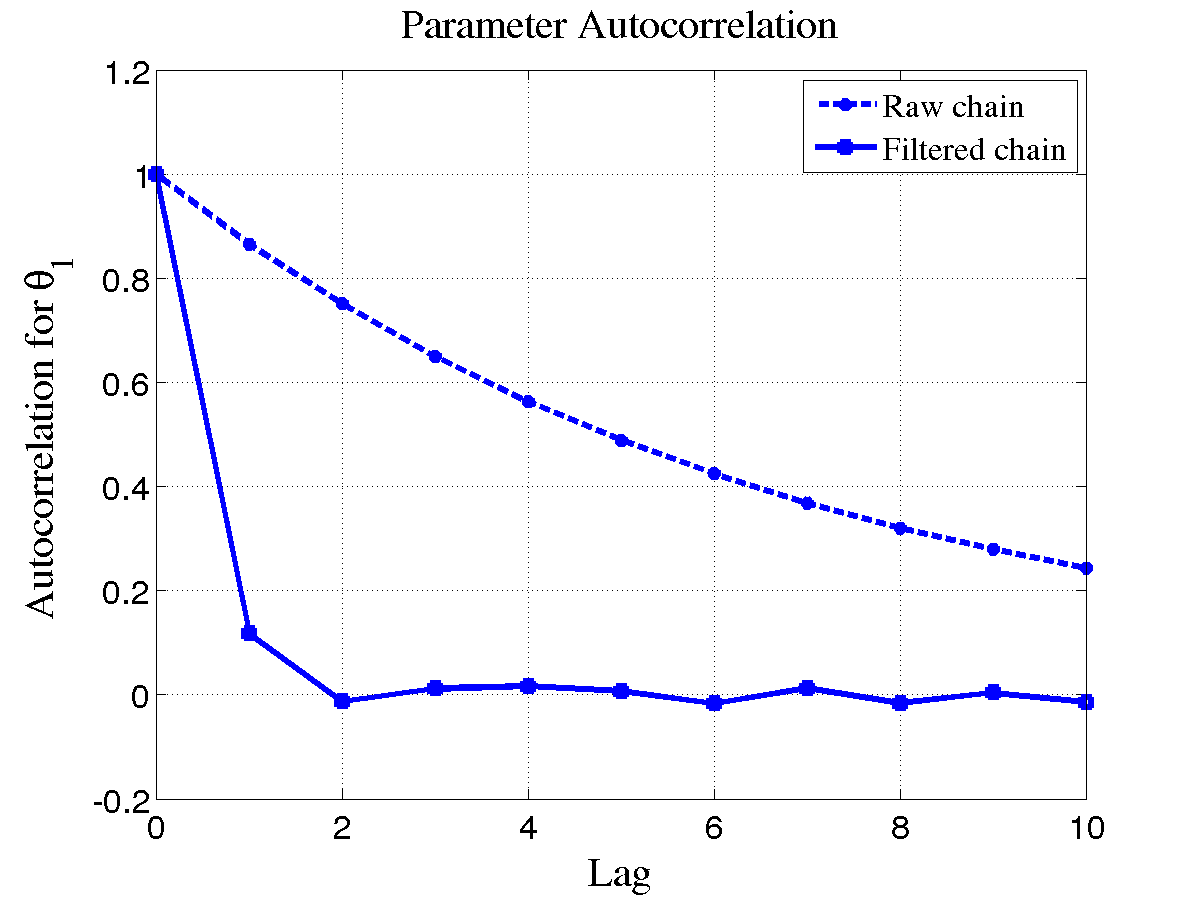
\includegraphics[scale=0.35]{figs/simple_ip_autocorrelation_raw_filt_theta1.png}}
%\subfloat[$\theta_2$]{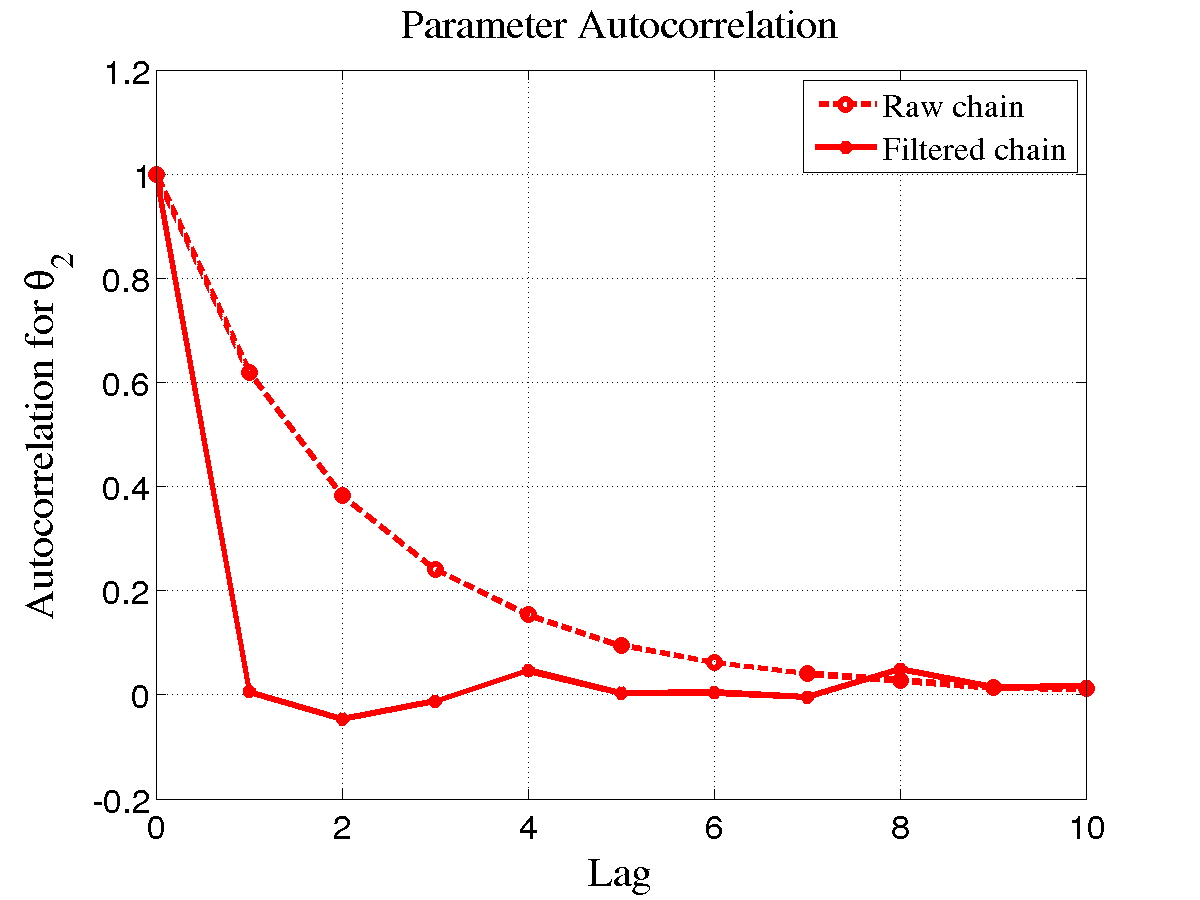
\includegraphics[scale=0.35]{figs/simple_ip_autocorrelation_raw_filt_theta2.png}}
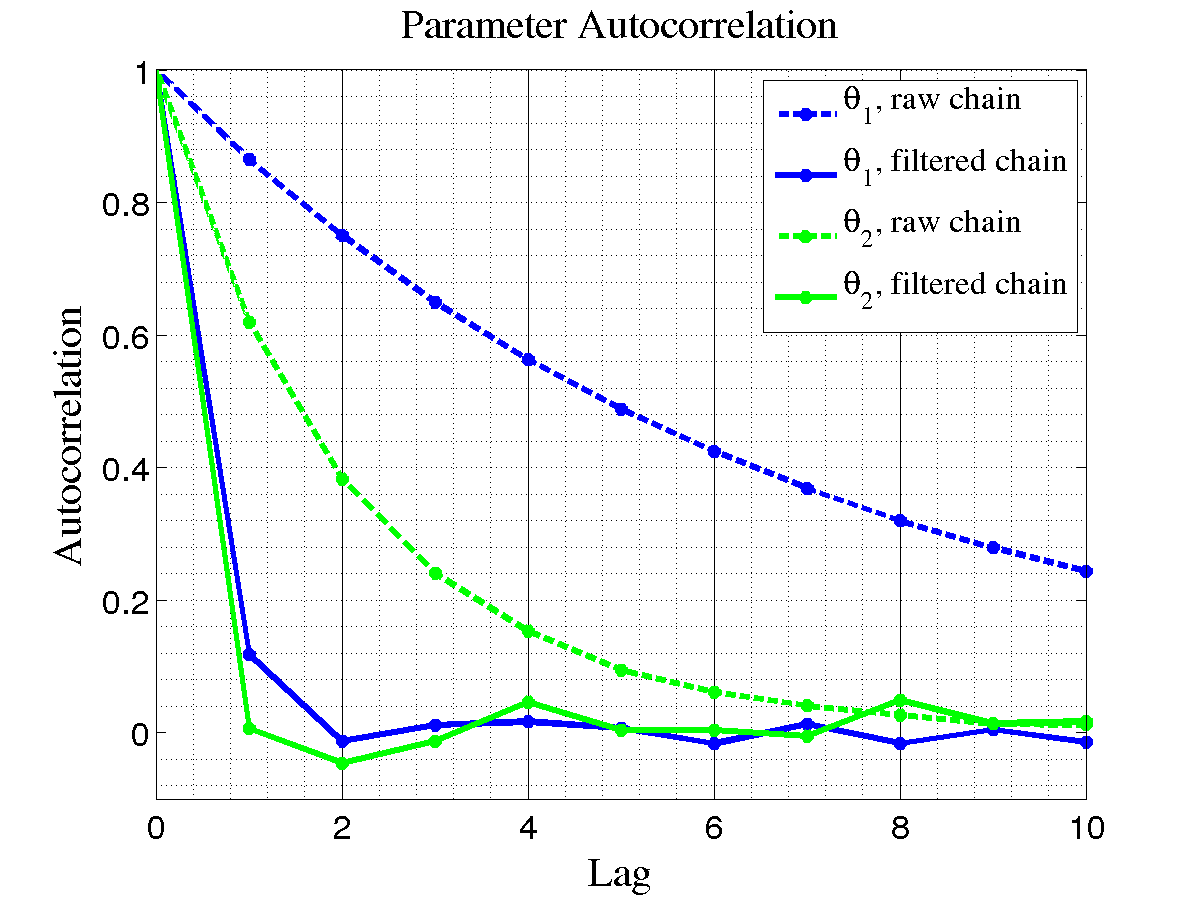
\includegraphics[scale=0.35]{figs/simple_ip_autocorrelation_raw_filt.png}
\vspace{-10pt}
\caption{
Autocorrelation plots obtained with QUESO for the SIP. }
\label{fig:simple_sip_autocorrelation_raw_filt}
\end{figure}


\subsubsection{KDE Plots}

Matlab function \verb+[f,xi] = ksdensity(x)+ (kernel smoothing density estimate) computes a probability density estimate of the sample in the vector \texttt{x}. \texttt{f} is the vector of density values evaluated at the points in \texttt{xi}. The estimate is based on a normal kernel function, using a window parameter (`width') that is a function of the number of points in \texttt{x}. The density is evaluated at 100 equally spaced points that cover the range of the data in x.  In order to estimate the KDE of the parameters, it is used together with the option `\verb+pdf+'. 

\begin{lstlisting}[label=matlab:ip_kde,caption={Matlab code for the KDE plots displayed in the left of Figure \ref{fig:simple_sip_kde}.}]
% Inside Matlab
% Raw chain
>> [f,x] = ksdensity(ip_mh_rawChain_unified(:,1),'function','pdf');
>> [f2,x2] = ksdensity(ip_mh_rawChain_unified(:,2),'function','pdf');
>> x_p1=sort(ip_mh_rawChain_unified(:,1)); %analytical
>> f_p1=(exp(-(x_p1+1).*(x_p1+1)/8))/2/sqrt(2*pi);
>> x_p2=sort(ip_mh_rawChain_unified(:,1));
>> f_p2=(exp(-(x_p2-2).*(x_p2-2)/2))/sqrt(2*pi);
>> plot(x,f,'b',x2,f2,'g','linewidth',4);
>> hold;
>> plot(x_p1,f_p1,'--k',x_p2,f_p2,'-k','linewidth',2);
>> h=legend('\theta_1', '\theta_2', 'analytical (\theta_1)', 'analytical (\theta_2)', 'location', 'northwest');
\end{lstlisting}

% \begin{lstlisting}[label=matlab:ip_kde,caption={Matlab code for the KDE plots displayed in Figure \ref{fig:simple_sip_kde}.}]
% % inside Matlab
% % theta_1
% >> [f,xi] = ksdensity(ip_mh_rawChain_unified(:,1),'function','pdf');
% >> x=ip_mh_rawChain_unified(:,1);
% >> x=sort(x);
% >> plot(x,(exp(-(x+1).*(x+1)/8))/2/sqrt(2*pi),'--k',xi,f,'-b','linewidth',3);
% >> title('Parameter Kernel Density Estimation (raw chain)','fontname', 'Times', 'fontsize',20);
% >> ylabel('Posterior marginal PDF','fontname', 'Times', 'fontsize',20);
% >> xlabel('\theta_1','fontname', 'Times', 'fontsize',20);
% >> h=legend('Analytical','QUESO','location','northeast');
% 
% % theta_2
% >> fprintf(1,' Plotting KDE - raw  <press any key>\n');
% >> [f,xi] = ksdensity(ip_mh_rawChain_unified(:,2),'function','pdf');
% >> x=ip_mh_rawChain_unified(:,2);
% >> x=sort(x);
% >> plot(x,(exp(-(x-2).*(x-2)/2))/sqrt(2*pi),'--k',xi,f,'-r','linewidth',3);
% >> title('Parameter Kernel Density Estimation (raw chain)','fontname', 'Times', 'fontsize',20);
% >> ylabel('Posterior marginal PDF','fontname', 'Times', 'fontsize',20);
% >> xlabel('\theta_2','fontname', 'Times', 'fontsize',20);
% >> h=legend('Analytical','QUESO','location','northeast');
% \end{lstlisting}

%Figure \ref{fig:sip_gravity_kde_raw} is created by using Matlab commands presented in Listing \ref{matlab:kde} above.
\begin{figure}[htpb]
\centering 
% \subfloat[]{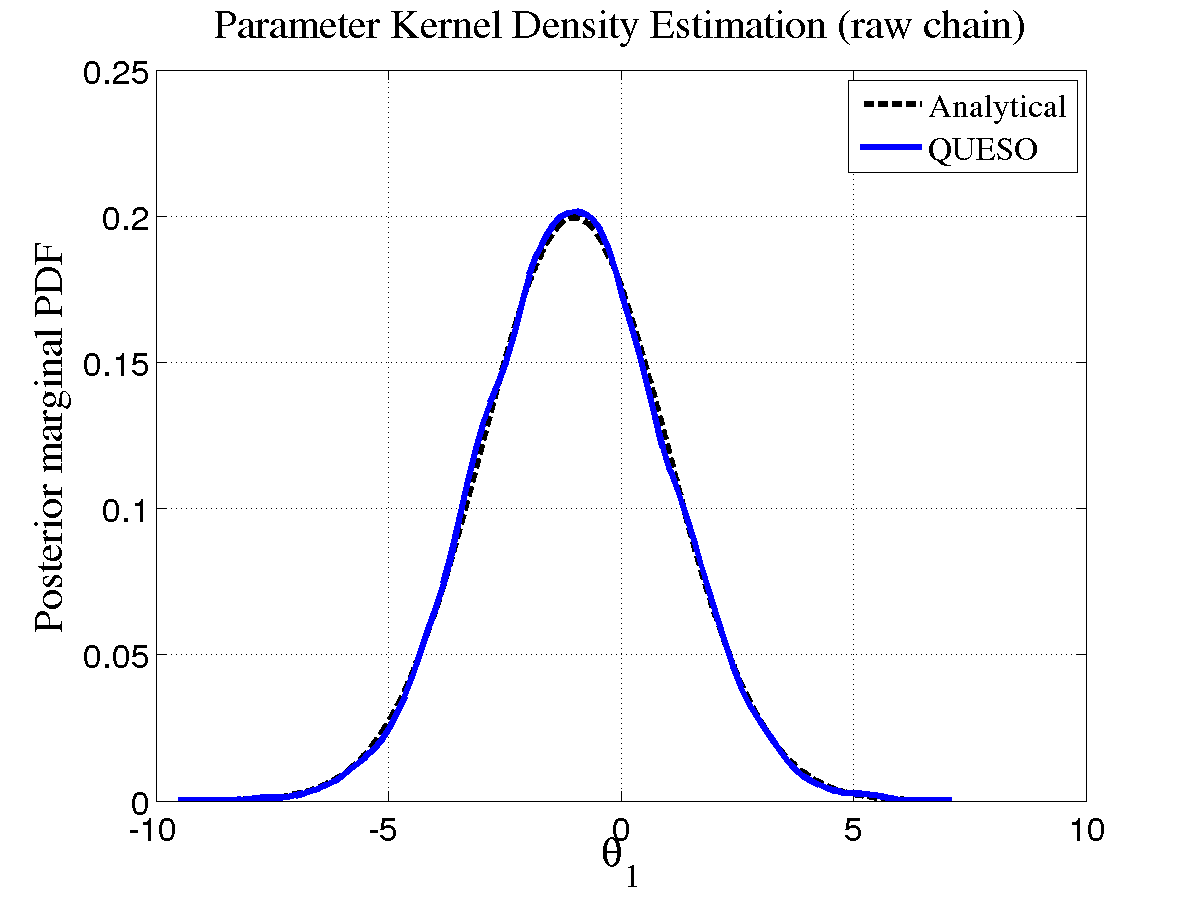
\includegraphics[scale=0.35]{figs/simple_ip_kde_theta1.png}}
% \subfloat[]{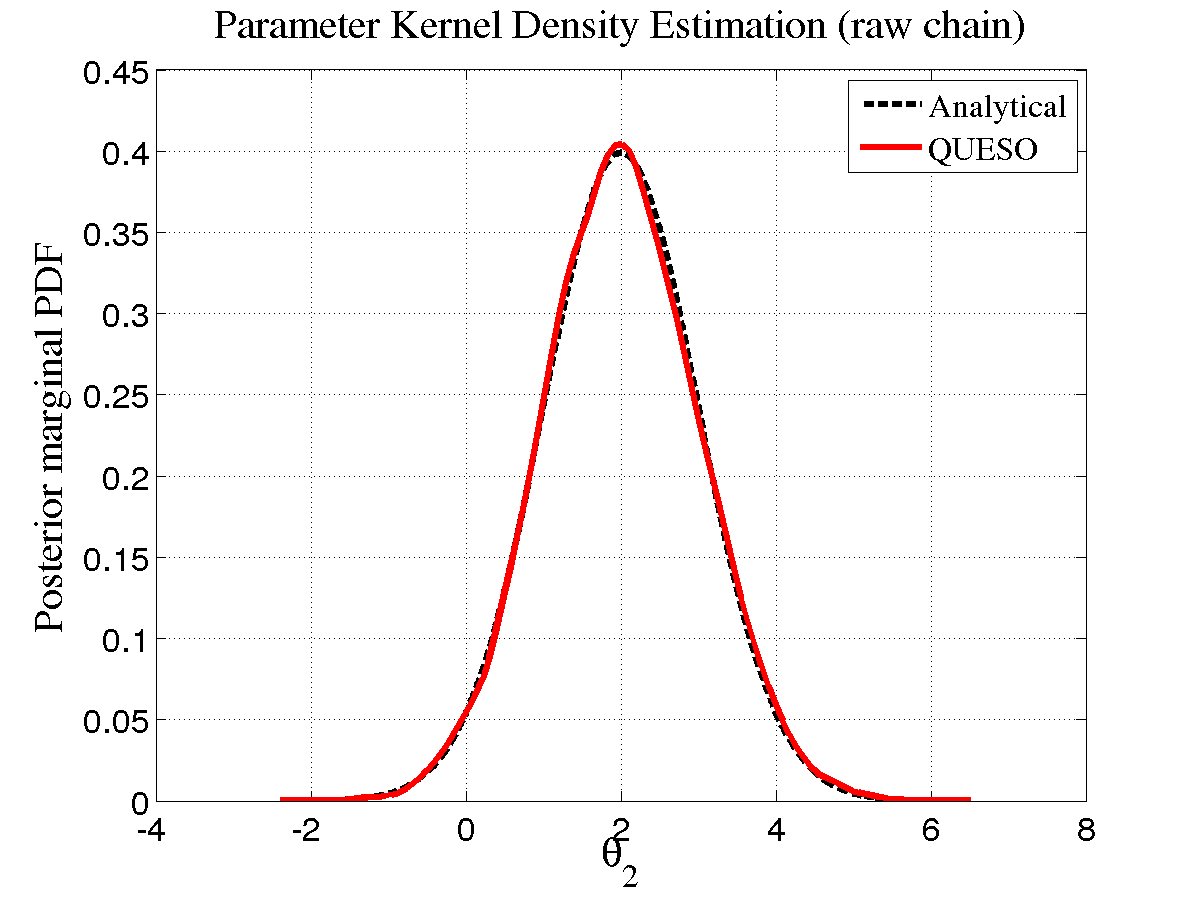
\includegraphics[scale=0.35]{figs/simple_ip_kde_theta2.png}}
\subfloat[Raw chain]{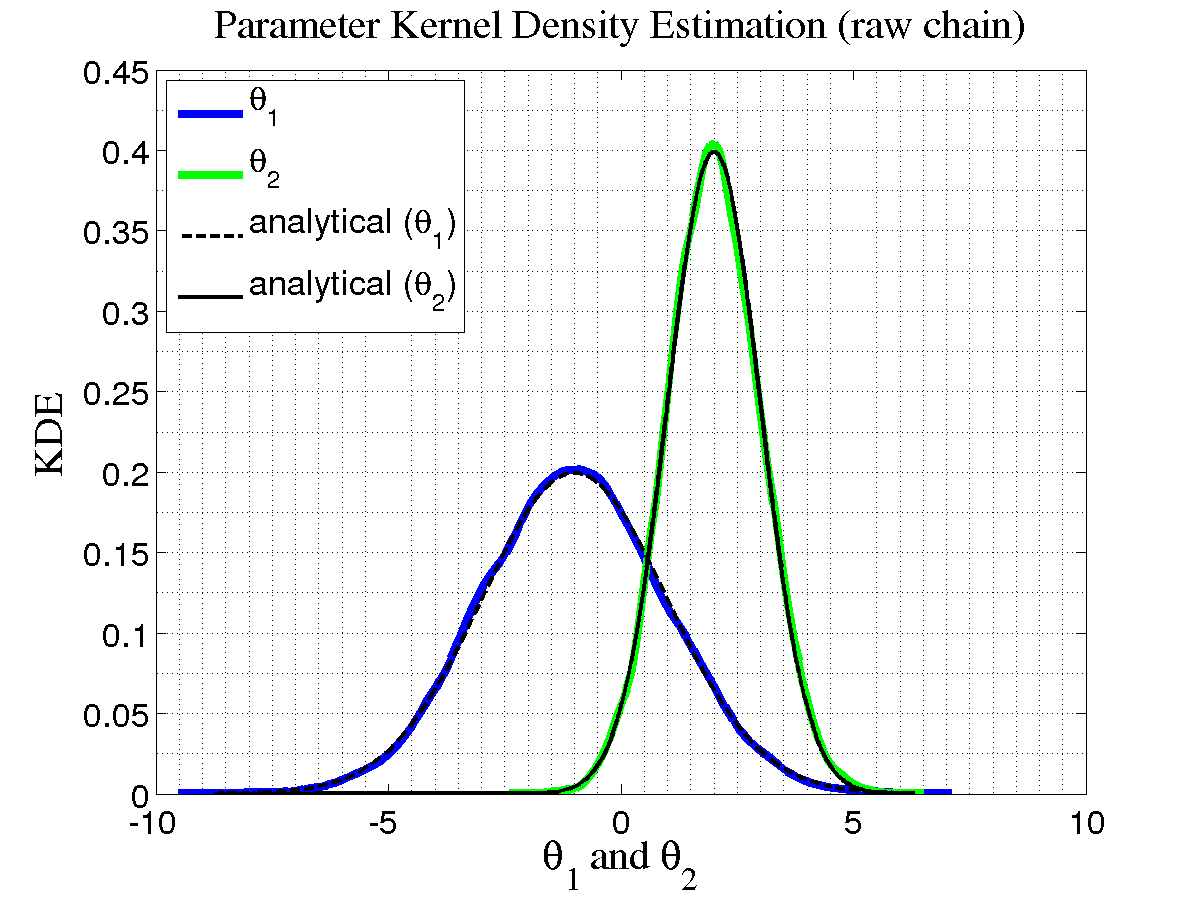
\includegraphics[scale=0.35]{figs/simple_ip_kde_raw.png}}
\subfloat[Filtered chain]{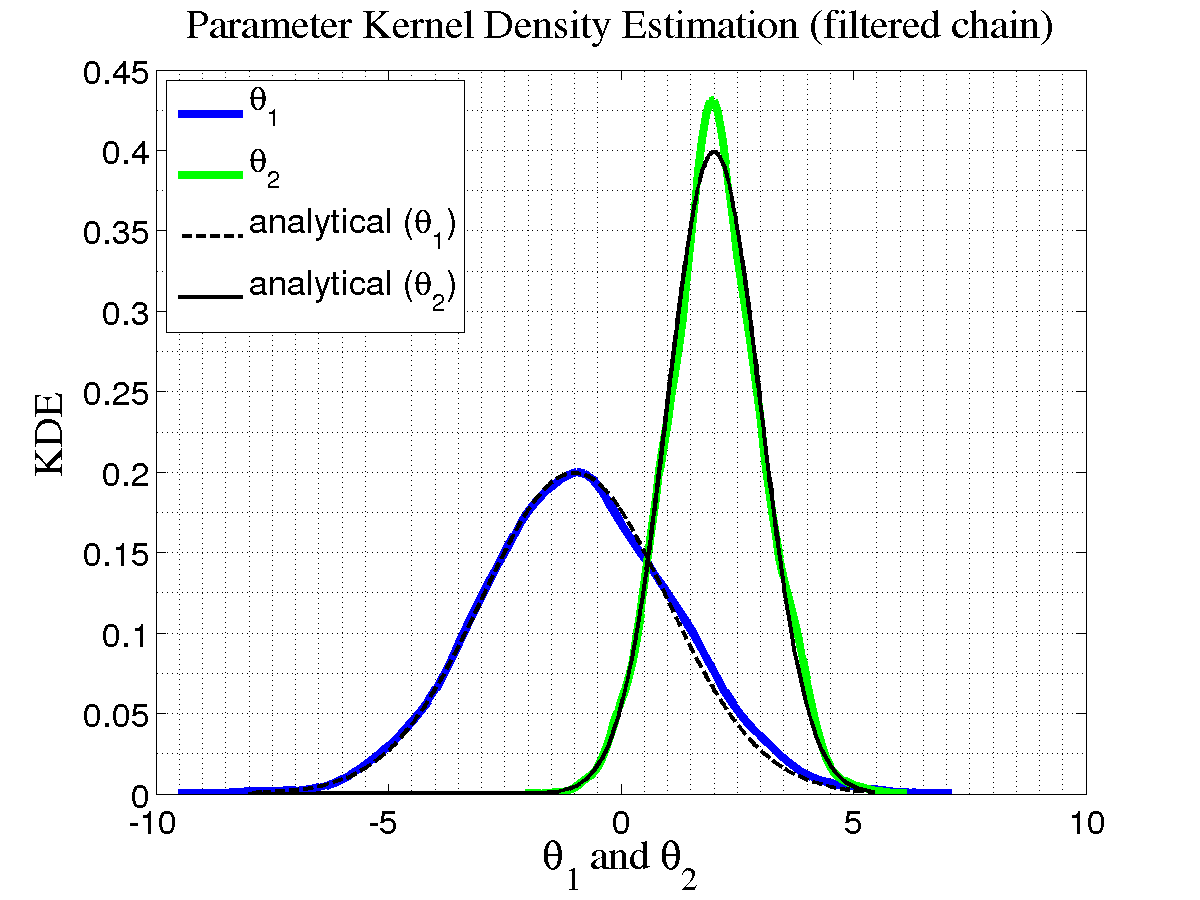
\includegraphics[scale=0.35]{figs/simple_ip_kde_filt.png}}
\vspace*{-10pt}
\caption{Kernel Density Estimation. QUESO results for estimation of the KDE of $\theta_1$ and $\theta_2$ are plotted against the analytical expressions $\pi_{\text{post}}(\theta_1)  =  \frac{1}{2\sqrt{2\pi}} \exp\left(-\frac{1}{8}(\theta_1+1)^2 \right)$  and $\pi_{\text{post}}(\theta_2)  =  \frac{1}{ \sqrt{2\pi}} \exp\left(-\frac{1}{2}(\theta_2-2)^2 \right)$, respectively.}
\label{fig:simple_sip_kde}
\end{figure}


\subsubsection{Covariance and Correlation Matrices}

Matlab function \verb+cov+ calculates the covariance matrix for a data matrix (where each column represents a separate quantity), 
and \verb+corr+ calculates the correlation matrix.

Listing \ref{matlab:cov_matrix} presents the Matlab steps for calculating the covariance and correlation matrices for the parameters $\theta_1$ and $\theta_2$.

\newpage

\begin{lstlisting}[label=matlab:ip_cov_matrix,caption={Matlab code for finding covariance and correlation matrices.}]
% inside Matlab
>> cov_matrix_theta1_theta2 = cov(ip_mh_rawChain_unified)

cov_matrix_theta1_theta2 =

    3.8729    0.0259
    0.0259    1.0050
    
>> corr_matrix_theta1_theta2 = corr(ip_mh_rawChain_unified)

corr_matrix_theta1_theta2 =

    1.0000    0.0132
    0.0132    1.0000    
\end{lstlisting}




\section{\texttt{simpleStatisticalForwardProblem}}\label{sec:example_sfp}

In this simple statistical forward problem (SFP), suppose that the quantity of interest $\mathbf{q}$ is a function of a random variable $\bv{\theta}$ of two parameters, namely $\bf{q}:\mathbb{R}^2\rightarrow\mathbb{R}$ such as:
\begin{equation}\label{eq-example-q}
\mathbf{q}(\boldsymbol{\theta}) = \theta_1+\theta_2,\quad\forall\boldsymbol{\theta}=(\theta_1,\theta_2)\in\mathbb{R}^2.
\end{equation}

Suppose also that the parameters in $\theta$ have Gaussian distribution with mean $\bv{\mu}$ and covariance matrix $\bf{C}$ given by:
\begin{equation}\label{eq-example-mu-sfp}
\boldsymbol{\mu} = 
\left(\begin{array}{c}
-1 \\
2
\end{array}\right)
\quad
\text{and}
\quad
\mathbf{C} = 
\left[\begin{array}{cc}
4 & 0 \\
0 & 1
\end{array}\right].
\end{equation}


Notice that since the solution $\mathbf{Q}$ of this SFP is the sum of two random variables $\boldsymbol{\Theta}_1$ and $\boldsymbol{\Theta}_2$, and since these two random variables independent Gaussian by assumption, should have:
\begin{equation}\label{eq-example-E}
E[\mathbf{Q}] = E[\boldsymbol{\Theta}_1] + E[\boldsymbol{\Theta}_2] = -1 + 2 = 1
\end{equation}
and
\begin{equation}\label{eq-example-V}
V[\mathbf{Q}] = V[\boldsymbol{\Theta}_1] + V[\boldsymbol{\Theta}_2] = 4 + 1 = 5
\end{equation}
where $E$ and $V$ indicate expectation and variance, respectively. Thus the analytical expression for the solution $\bf{Q}$ is this SFP is the one-dimensional Gaussian distribution of mean 1 and variance 5:
\begin{equation}\label{eq-example-sfp-analytical}
{\bf Q}(x)=   \frac{1}{ \sqrt{10\pi}} \exp\left(-\frac{1}{10}(x-1)^2 \right)
\end{equation}


In this example, we use QUESO Monte Carlo algorithm to sample from the QoI given in Equation (\ref{eq-example-q}) and analyze it. 
Since the parameters have known independent Gaussian distributions, the results obtained by QUESO via sampling the QoI, in Equation (\ref{eq-example-q}), should match the Gaussian distribution given in Equation (\ref{eq-example-sfp-analytical}).


\paragraph*{Note:} Due to the possibility to compare QUESO sampling algorithms to an analytical expression, this example is also used in the verification procedures and regression tests within QUESO. In fact it is the second part of the test \verb+tests/t02_sip_sfp+.


\subsection{Running the Example}\label{sec:sfp-run}
 
To run the executable provided (available after QUESO installation), enter the following commands:
\begin{lstlisting}[label={},caption={}]
$ cd $HOME/LIBRARIES/QUESO-0.47.1/
$ cd examples/simpleStatisticalForwardProblem
$ rm outputData/*
$ ./exSimpleStatisticalForwardProblem_gsl example.inp    
$ matlab
   $ simple_fp_plots      # inside matlab
   $ exit                 # inside matlab
$ ls -l outputData/*.png
 simple_fp_autocorrelation_qoi.png  simple_fp_chain_pos_param.png  
 simple_fp_hist_qoi.png             simple_fp_cdf_qoi.png
 simple_fp_chain_pos_qoi.png        simple_fp_kde_qoi.png
\end{lstlisting}

As a result, the user should have created several of PNG figures containing marginal posterior PDF, chain positions of the parameters and the QoI, histogram, cumulative density distribution and autocorrelation. The name of the figure files have been chosen to be informative, as shown in the Listing above.



\subsection{Example Code}\label{sec:code-sfp}

The source code for the SFP example is composed of 5 files:
\texttt{simple\_sfp\_example\_main.C} (Listing~\ref{code:sfp-main-c}),
\texttt{simple\_sfp\_example\_qoi.h} and \texttt{simple\_sfp\_example\_qoi.C} (Listings \ref{code:sfp-qoi-h} and~\ref{code:sfp-qoi-c}),
\texttt{simple\_sfp\_example\_compute.h}  and \texttt{simple\_sfp\_example\_compute.C} (Listings \ref{code:sfp-compute-h} and \ref{code:sfp-compute-c}).


\lstinputlisting[caption=File \texttt{simple\_sfp\_example\_main.C.}, label={code:sfp-main-c}, linerange={29-1000}]{../../examples/simpleStatisticalForwardProblem/src/simple_sfp_example_main.C}

\lstinputlisting[caption=File \texttt{simple\_sfp\_example\_qoi.h}., label={code:sfp-qoi-h}, linerange={28-1000}]{../../examples/simpleStatisticalForwardProblem/src/simple_sfp_example_qoi.h}

\lstinputlisting[caption=File \texttt{simple\_sfp\_example\_qoi.C}., label={code:sfp-qoi-c}, linerange={29-1000}]{../../examples/simpleStatisticalForwardProblem/src/simple_sfp_example_qoi.C}

\lstinputlisting[caption=File \texttt{simple\_sfp\_example\_compute.h.}, label={code:sfp-compute-h}, linerange={28-1000}]{../../examples/simpleStatisticalForwardProblem/src/simple_sfp_example_compute.h}

\lstinputlisting[caption={File \texttt{simple\_sfp\_example\_compute.C}.}, label={code:sfp-compute-c}, linerange={29-1000},numbers=left]{../../examples/simpleStatisticalForwardProblem/src/simple_sfp_example_compute.C}
 


\subsection{Input File}\label{sec:sfp-input-file}

In the case of a SFP, QUESO expects a list of options for Monte Carlo algorithm,
together with options for QUESO environment; such as the name of the output files and which sub-environments will write to to them. 
Note that the names of the variables have been designed to be informative:
\begin{description}\vspace{-8pt}
\item[ \texttt{env}:] refers to QUESO environment; \vspace{-8pt}
\item[ \texttt{fp}:] refers to forward problem;\vspace{-8pt}
\item[ \texttt{mc}:] refers to Monte Carlo;\vspace{-8pt}
\item[ \texttt{pseq}:] refers to the parameter sequence; and\vspace{-8pt}
\item[ \texttt{qseq}:] refers to the quantity of interest sequence.
\end{description}

The options used for solving this simple SFP are displayed in Listing \ref{code:sfp-input-file}.


\lstinputlisting[caption={File name \texttt{simple\_sfp\_example.inp} with options for QUESO library used in application code (Listings \ref{code:sfp-main-c}--\ref{code:sfp-compute-c}})., 
label={code:sfp-input-file},]{../../examples/simpleStatisticalForwardProblem/tests/test_2013_08_27/simple_sfp_example.inp}



\subsection{Create your own Makefile}\label{sec:sfp-makefile}

 
Listing \ref{code:makefile} presents a Makefile, named `\texttt{Makefile\_sfp\_example\_margarida}', that may be used to compile the code and create the executable \verb+simple_sfp_example+. Naturally, it must be adapted to the user's settings, i.e., it has to have the correct paths for the user's libraries that have actually been used to compile and install QUESO.

\lstinputlisting[caption={Makefile for the application code in Listings \ref{code:sfp-main-c}--\ref{code:sfp-compute-c}},  label={code:sfp-makefile},language={bash}]{../../examples/simpleStatisticalForwardProblem/src/Makefile_sfp_example_margarida}

Thus, to compile, build and execute the code, the user just needs to run the following commands in the same directory where the files are:
\begin{lstlisting}
$ cd HOME/LIBRARIES/QUESO-0.47.1/examples/simpleStatisticalForwardProblem 
$ export LD_LIBRARY_PATH=$LD_LIBRARY_PATH:\
  $HOME/LIBRARIES/gsl-1.15/lib/:\
  $HOME/LIBRARIES/boost-1.53.0/lib/:\
  $HOME/LIBRARIES/hdf5-1.8.10/lib:\
  $HOME/LIBRARIES/QUESO-0.47.1/lib 
$ make -f Makefile_sfp_example_margarida 
$ ./simple_sfp_example simple_sfp_example.inp
\end{lstlisting}

The `\verb+export+' instruction above is only necessary if the user has not saved it in his/her \verb+.bashrc+ file. 


\subsection{Data Post-Processing and Visualization}\label{sec:sfp-results}

This section discusses the results computed by QUESO with the code of Section \ref{sec:code-sfp}, and shows how to use Matlab for the post-processing of the data generated by QUESO when solving SFPs. Only the essential Matlab commands are presented; for the complete/detailed codes, please refer to file '\verb+simple_fp_plots.m+'.

According to the specifications of the input file in Listing~\ref{code:sfp-input-file}, a folder named `\verb+outputData+' containing the following files should be created: \verb+display_sub0.txt, fp_p_seq.m,+ \linebreak \verb+fp_p_seq_sub0.m, fp_q_seq.m, fp_q_seq_sub0.m,+ and \verb+sfpOutput_sub0.m+.

The code bellow shows how to load the data provided by QUESO during the solution process of the SFP described, in the form of chains of positions.
\begin{lstlisting}[caption={Matlab code for loading the data in both parameter and QoI chains of the SFP.}]
% inside Matlab
>> clear all
>> fp_p_seq.m
>> fp_q_seq.m
\end{lstlisting}


Alternatively, the user may call the file \texttt{simple\_fp\_plots.m}, which contains the above commands, together with a variety of others, for data visualization:
\begin{lstlisting}[caption={Matlab code for loading the data in both parameter and QoI chains of the SFP, by calling the file \texttt{simple\_fp\_plots.m}.}]
% inside Matlab
>> clear all
>> simple_fp_plots
\end{lstlisting}




\subsubsection{Histogram Plots}

In order to plot a histogram of the QoI, you may use the pre-defined Matlab function \verb+hist+.
The Matlab code presented in Listing \ref{matlab:fp_hist_qoi} below shows how to create the Figure~\ref{fig:fp_qoi_hist}.

\begin{lstlisting}[label=matlab:fp_hist_qoi,caption={Matlab code for the QoI histogram plot.}]
% inside Matlab
>> fp_q_seq  %if commands of Listings 3.19/3.20 have not been called
>> nbins=20;
>> hist(fp_mc_QoiSeq_unified,nbins);
>> title('QoI Histogram','fontsize',20);
>> xlabel('QoI=\theta_1+\theta_2','fontname', 'Times', 'fontsize',20)
>> ylabel('Frequency','fontsize',20);
\end{lstlisting}

\begin{figure}[htb]
\centering 
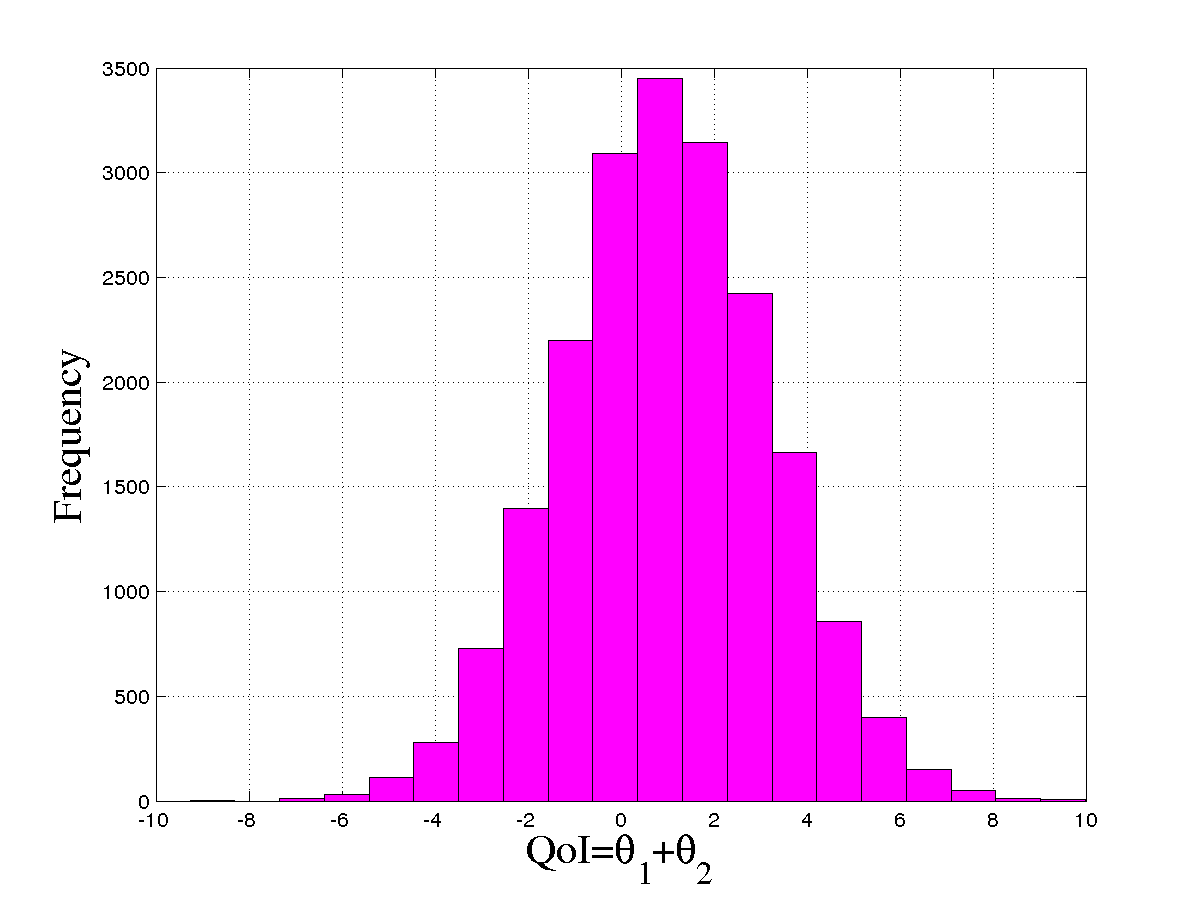
\includegraphics[scale=0.35]{figs/simple_fp_hist_qoi.png}
\vspace{-10pt}
\caption{QoI histogram.}
\label{fig:fp_qoi_hist}
\end{figure}

\subsubsection{KDE Plot}

Matlab function \verb+ksdensity+ (Kernel smoothing density estimate) together with the option `\verb+pdf+' may be used to estimate the KDE of the QoI. 

\begin{lstlisting}[label=matlab:fp_kde_qoi,caption={Matlab code for the KDE displayed in Figure \ref{fig:simple_sfp_kde}}]
% inside Matlab
>> fp_q_seq  %if commands of Listing 5.19 have not been called
>> [fi,xi] = ksdensity(fp_mc_QoiSeq_unified,'function','pdf');
>> x=sort(fp_mc_QoiSeq_unified);
>> mu=1;
>> sigma2=5;
>> f=(exp(-(x-mu).*(x-mu)/sigma2/2))/sqrt(2*pi*sigma2);
>> plot(xi,fi,'-m','linewidth',4);
>> hold;
>> plot(x,f,'--k','linewidth',2);
>> h=legend('QoI = \theta_1+\theta_2','analytical','location','northwest');
\end{lstlisting}


%Figure \ref{fig:sip_gravity_kde_raw} is created by using Matlab commands presented in Listing \ref{matlab:kde} above.
\begin{figure}[htpb]
\centering 
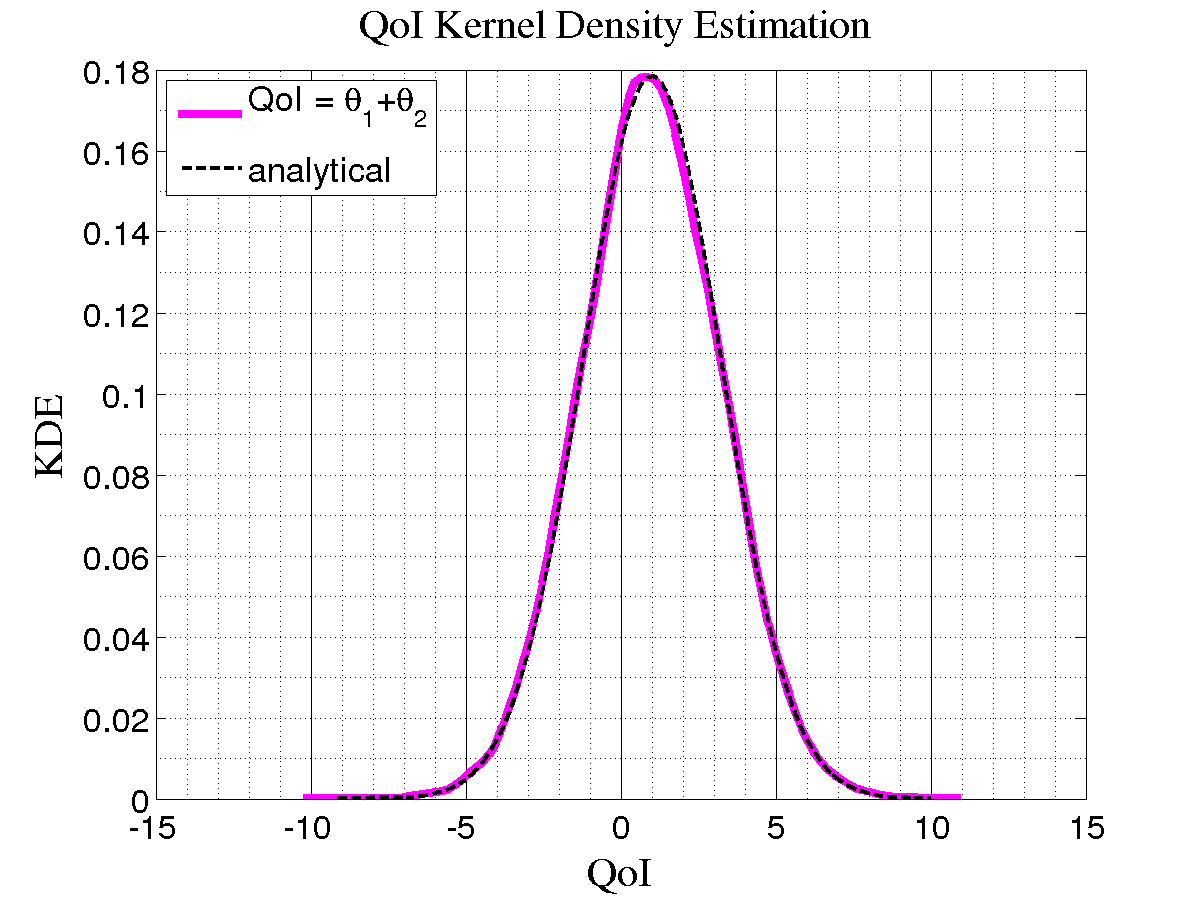
\includegraphics[scale=0.35]{figs/simple_fp_kde_qoi.png}
\vspace{-10pt}
\caption{Kernel Density Estimation. QUESO results are plotted against the PDF of a Gaussian distribution $Q(x)=   \frac{1}{ \sqrt{10\pi}} \exp\left(-\frac{1}{10}(x-1)^2 \right)$, where $\mu=1$ and $\sigma^2=5$.}
\label{fig:simple_sfp_kde}
\end{figure}


\subsubsection{CDF Plot}

Matlab function \verb+ksdensity+ with \verb+'cdf'+ option may also be used for plotting the Cumulative Distribution Function of the QoI.

\begin{lstlisting}[label=matlab:fp_cdf_qoi,caption={Matlab code for the QoI CDF plot displayed in Figure \ref{fig:simple_sfp_cdf}.}]
% inside Matlab
>> fp_q_seq  %if commands of Listing 5.19 have not been called
>> [f,xi] = ksdensity(fp_mc_QoiSeq_unified,'function','cdf');
>> plot(xi,f,'-m','linewidth',3)
\end{lstlisting}

\begin{figure}[htpb]
\centering 
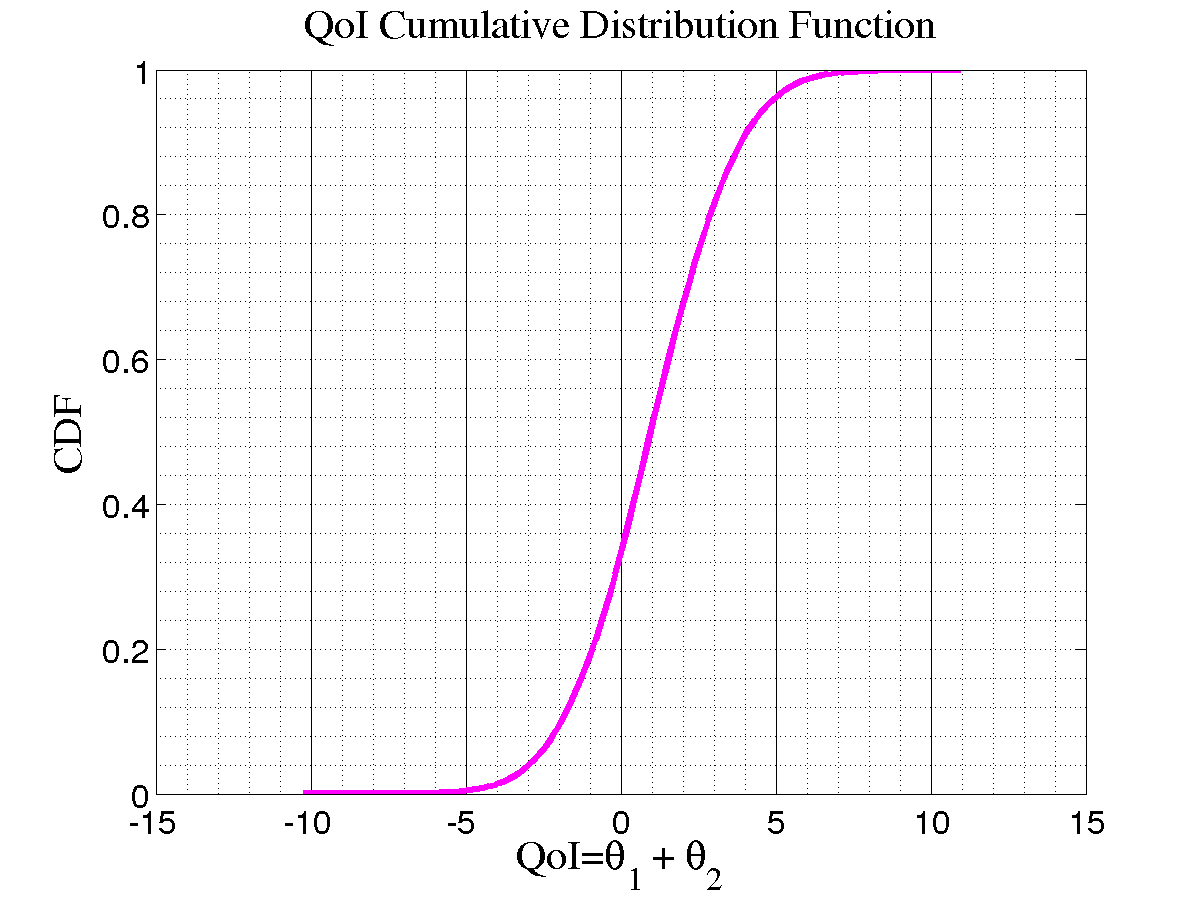
\includegraphics[scale=0.35]{figs/simple_fp_cdf_qoi.png}
\vspace*{-10pt}
\caption{Cumulative Distribution Function.}
\label{fig:simple_sfp_cdf}
\end{figure}



\section{\texttt{gravity}}\label{sec:example_gravity}

This section presents an example of how to use QUESO in order to develop an application that solves a statistical inverse problem and
a statistical forward problem, where the solution of the former serves as input to the later. During the SIP, the acceleration due to gravity for an object in free fall near the surface of the Earth is inferred. During the SFP, the distance traveled by a projectile launched at a given angle and altitude is calculated using the calibrated magnitude of the acceleration of gravity.


In this section we describe a statistical forward problem  of predicting the  described in Section \ref{sec:gravity-ip}.

\subsection{Statistical Inverse Problem}\label{sec:gravity-ip}

% Near the surface of the Earth, an object in free fall in a vacuum will accelerate at approximately $9.8 m/s^2$, independent of its mass.
% With air resistance acting upon an object that has been dropped, mass, drag coefficient and even relative surface may become important
% (if the fall is from sufficient altitude) in the calculation of gravity.

%The vertical motion of an object falling a small distance close to the surface of the planet can be approximated to have
%uniform gravitational field without air resistance, as long as the force of gravity on the object is much greater than the force of air resistance.

%Therefore a convenient, simplified 
A possible deterministic mathematical model for the vertical motion of an object in free fall near the surface of the Earth is given by
\begin{equation}\label{eq:gravity01}
h(t)=-\frac{1}{2} g t^2 + v_0 t + h_0.
\end{equation}
where
$v_0$ [$m/s$] is the initial velocity,
$h_0$ [$m$] is the initial altitude,
$h(t)$ [$m$] is the altitude with respect to time,
$t$ [$s$] is the elapsed time, and
$g$ [$m/s^2$] is the magnitude of the acceleration due to gravity (the parameter which cannot be directly measured and will be statistically inferred).



\subsubsection{Experimental Data}
We assume that the experiment of allowing an object to fall from different altitudes with zero initial velocity has been repeatedly conducted (See Figure \ref{fig:free_fall}). The data collected, e.g.  $\mathbf{d}$, is displayed in Table \ref{table:data}; the standard deviations, $\sigma$'s, refer to the uncertainties in the measured times during the experiment execution~\cite{interactagram}. 



\begin{figure}[!h]
\centering
\input{rawfigs/free_fall.latex}
\vspace*{-8pt}
\caption{An object falls from altitude $h_0$ with zero initial velocity ($v_0=0$).}
\label{fig:free_fall}
\end{figure}

\begin{table}[htp]%% Data from data02.dat 
\caption{Measurement data $\mathbf{d}$ of size $n_d=14$.
The object falls from altitude $h_0$ in $t$ seconds, with standard deviation of $\sigma$ seconds in the time measurement~\cite{interactagram}.
}
% \specialrule{.4pt}{10pt}{4pt}
\vspace{-8pt}
\begin{center}
\begin{tabular}{ccc}
\toprule
% $(h_0-h)$ [$m$] & $t$ [$s$]  & $\sigma$ [$s$]\\
altitude [$m$] & time [$s$]  & Std. Dev. $\sigma$ [$s$]\\
\midrule
\midrule
$~$10	&	1.41	&	0.02	\\
$~$20	&	2.14	&	0.12	\\
$~$30	&	2.49	&	0.02	\\
$~$40	&	2.87	&	0.01	\\
$~$50	&	3.22	&	0.03	\\
$~$60	&	3.49	&	0.01	\\
$~$70	&	3.81	&	0.03	\\
$~$80	&	4.07	&	0.03	\\
$~$90	&	4.32	&	0.03	\\
100	&	4.47	&	0.05	\\
110	&	4.75	&	0.01	\\
120	&	4.99	&	0.04	\\
130	&	5.16	&	0.01	\\
140	&	5.26	&	0.09	\\
\bottomrule
\end{tabular}
\end{center}
\label{table:data}
\end{table}



\subsubsection{The Prior RV, Likelihood and Posterior RV}

In a straightforward classical interpretation of Bayesian inference, the prior signifies the modeler's honest opinion about the unknown.
For the gravity inference problem, let's assume that gravity varies uniformly in the interval [8,11], or, in other words, we chose uniform prior distribution in that interval:

\begin{equation}\label{eq-g-prior}
\pi_{\text{prior}}=\mathcal{U}(8,11).
\end{equation}


We choose the usual likelihood function:
\begin{equation}\label{eq:like02}
\pi_{\text{like}}(\mathbf{d} | \boldsymbol{\theta})
\varpropto
\exp
\left\{
-\frac{1}{2}
[\mathbf{y}(\boldsymbol{\theta})-\mathbf{d}]^T
\left[\mathbf{C}(\boldsymbol{\theta})\right]^{-1}
[\mathbf{y}(\boldsymbol{\theta})-\mathbf{d}]
\right\},
\end{equation}
where $\mathbf{C}(\boldsymbol{\theta})$ is a given covariance matrix, $\mathbf{d}$ denotes experimental data, $\mathbf{y}(\boldsymbol{\theta})$ is the model output data.

Recalling the deterministic model for the acceleration of gravity (\ref{eq:gravity01}) with zero initial velocity,  the information provided in Table \ref{table:data}, and Equation (\ref{eq:like02}); and, additionally, invoking the nomenclature used in Section \ref{sec:statistical_concepts}, we have:
\begin{equation}\label{eq:like03}
\boldsymbol{\theta} \stackrel{\text{\small{def.}}}{=} g,
%------------ 
\quad
\mathbf{y}(\boldsymbol{\theta})= 
\left[
\begin{array}{c}
\sqrt{\dfrac{2 h_1}{g}}\\	
\sqrt{\dfrac{2 h_2}{g}}\\	
\vdots\\	
\sqrt{\dfrac{2 h_{n_d}}{g}}
\end{array}
\right],
%------------ 
\quad 
\mathbf{d} = 
\left[
\begin{array}{c}
t_1    \\
t_2    \\ 
\vdots \\	
t_{n_d}
\end{array}
\right],
%------------ 
\quad
\mathbf{C}(\boldsymbol{\theta})=
\left[
\begin{array}{cccc}
\sigma^2_1 & 0	        & \cdots & 0 \\
0          & \sigma^2_2 & \cdots & 0 \\
\vdots     & \vdots     & \ddots & 0 \\
0          & 0          & \cdots & \sigma^2_{n_d}
\end{array}
\right],
\end{equation}
where $n_d=14$ is the number of data points in Table \ref{table:data}.

Now we are ready to evoke Bayes' formula in order to obtain the posterior PDF $\pi_{\text{post}}(\boldsymbol{\theta})$:
\begin{equation}\label{eq-Bayes-g}
\pi_{\text{post}}(\boldsymbol{\theta}|\mathbf{d})\varpropto  \pi_{\text{like}}(\mathbf{d}|\boldsymbol{\theta}) \, \pi_{\text{prior}}(\boldsymbol{\theta}).
\end{equation}


\subsection{Statistical Forward Problem}


Projectile motion refers to the motion of an object projected into the air at an angle, e.g. a soccer ball being kicked, a baseball being thrown, or an athlete long jumping. Supposing the object does not have a propulsion system and neglecting air resistance, then the only force acting on the object is a constant gravitational acceleration $g$.


A possible deterministic two-dimensional mathematical model for the vertical motion of an object projected from near the surface of the Earth is given by
\begin{align}\label{eq:fwd01}
v_x &= v_{0x} \\ %&= v_{0} \cos(\alpha), \\
v_y &= v_{0y} - gt \\ %&= v_{0} \sin(\alpha) - gt,\\
  x &= v_{0x}t \\ %&= v_{0} \cos(\alpha) t, \\
  h &= h_0 + v_{0y}t - \frac{1}{2} g t^2  %&= v_{0} \sin(\alpha) t - \frac{1}{2} g t^2.
\end{align}
where
$h_0$ is the initial height, $x=x(t)$ is the distance traveled by the object, $\bv{v_0}=(v_{0x},v_{0y})$ is the initial velocity,
$v_{0x} = v_{0} \cos(\alpha)$, $v_{0y} = v_{0} \sin(\alpha)$, and $v_0=\|\bv{v_0}\|^2$.
%
Figure \ref{fig:projectile} displays the projectile motion of an object in these conditions.
\begin{figure}[!h]
\centering
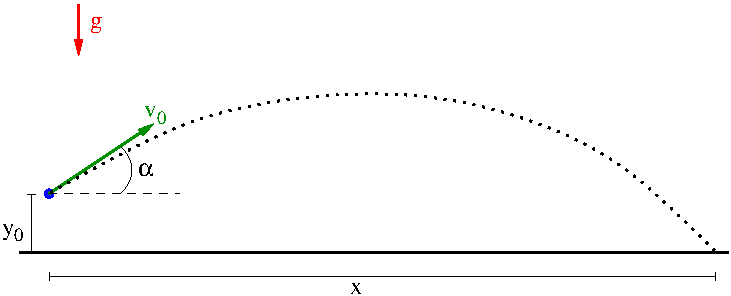
\includegraphics[scale=1]{figs/projectile}
\vspace*{-8pt}
\caption{Object traveling with projectile motion. }
\label{fig:projectile}
\end{figure}


%Assume that we want to describe the motion of such an object, starting at time $t = 0$, ... and velocity that makes an angle $\alpha$ with the $x$-axis.


For this example, we assume that $h_0 =0$ m, $\alpha = \pi/4$ radians, $v_0 = 5$ m/s, all deterministic variables; and $g$ is the solution of the SIP described in Section \ref{sec:gravity-ip}.

Since a PDF is assigned to parameter $g$; thus, the output of the mathematical model (\ref{eq:fwd01}) becomes a random variable, thus we have a statistical forward problem. 

\subsubsection{The Input RV, QoI Function and Output RV}
 
The input random variable for the statistical forward problem is the acceleration of gravity $g$, which is also the solution (posterior PDF) of the inverse problem described in Section \ref{sec:gravity-ip}. The output random variable for this example is the distance $x$ traveled by an object in projectile motion. Note that, since there is uncertainty in the parameter $g$ ($g$ is given as a PDF), one can expect that this uncertainty will be propagated to $x$, which will also be given as a PDF.

Combining the expressions in Equation \ref{eq:fwd01} and rearranging them, we have that QoI function for $x$ %(i.e. the final model for the distance traveled by an object in projectile motion) 
is: 
\begin{equation}\label{eq:fp_deterministic}
x=\dfrac{ v_0 \cos \alpha }{g} \left( v_0  \sin \alpha  + \sqrt{ ( v_0  \sin \alpha)^2 + 2g\, y_0 }\right).                                                                                        
\end{equation}
where $y$ is the distance traveled and our quantity of interest (QoI). 



\subsection{Running the Example}\label{sec:gravity-run}
 
To run the executable provided (available after QUESO installation), enter the following commands:
\begin{lstlisting}[label={},caption={}]
$ cd $HOME/LIBRARIES/QUESO-0.47.1/examples/gravity
$ rm outputData/*
$ ./gravity_gsl gravity_inv_fwd.inp
\end{lstlisting}

The console output of the program is:
\begin{lstlisting}[caption={Console output of program \texttt{gravity\_gsl}}, label={code:console_output},language={bash}]
kemelli@violeta:~/LIBRARIES/QUESO-0.47.1/examples/gravity$ ./gravity_gsl gravity_inv_fwd.inp 
---------------------------------------------------------------------
QUESO Library: Version = 0.47.1 (47.1)

Development Build

Build Date   = 2013-04-29 17:05
Build Host   = violeta
Build User   = kemelli
Build Arch   = x86_64-unknown-linux-gnu
Build Rev    = 38998M

C++ Config   = mpic++ -g -O2 -Wall

Trilinos DIR = 
GSL Libs     = -L/home/kemelli/LIBRARIES/gsl-1.15/lib -lgsl -lgslcblas -lm
GRVY DIR     = 
GLPK DIR     = 
HDF5 DIR     = /home/kemelli/LIBRARIES/hdf5-1.8.10
--------------------------------------------------------------------------------------------------------------
Beginning run at Mon Apr 29 17:27:32 2013

MPI node of worldRank 0 has fullRank 0, belongs to subEnvironment of id 0, and has subRank 0
MPI node of worldRank 0 belongs to sub communicator with full ranks 0
MPI node of worldRank 0 also belongs to inter0 communicator with full ranks 0, and has inter0Rank 0


Beginning run of 'Gravity + Projectile motion' example at Mon Apr 29 17:27:32 2013

 my fullRank = 0
 my subEnvironmentId = 0
 my subRank = 0
 my interRank = 0

Beginning 'SIP -> Gravity estimation' at Mon Apr 29 17:27:32 2013

Solving the SIP with Metropolis Hastings

Beginning 'SFP -> Projectile motion' at Mon Apr 29 17:27:33 2013

Solving the SFP with Monte Carlo

Ending run of 'Gravity + Projectile motion' example at Mon Apr 29 17:27:33 2013

Ending run at Mon Apr 29 17:27:33 2013
Total run time = 1 seconds
kemelli@violeta:~/LIBRARIES/QUESO-0.47.1/examples/gravity$ 
\end{lstlisting}


In order to generate chain plots, histograms, KDEs, etc., the user may use Matlab/GNU Octave and call the following command lines:
\begin{lstlisting}
$ matlab
   $ gravity_plots_ip      # inside matlab
   $ gravity_plots_fp      # inside matlab
   $ exit                  # inside matlab
$ ls -l outputData/*.png
  sfp_gravity_autocorrelation.png  sfp_gravity_cdf.png
  sfp_gravity_chain_pos.png        sfp_gravity_hist.png
  sfp_gravity_kde.png              sip_gravity_autocorrelation_raw_filt.png
  sip_gravity_cdf_filt.png         sip_gravity_cdf_raw.png
  sip_gravity_chain_pos_filt.png   sip_gravity_chain_pos_raw.png
  sip_gravity_hist_filt.png        sip_gravity_hist_raw.png
  sip_gravity_kde_filt.png         sip_gravity_kde_raw.png
\end{lstlisting}

As a result, the user should have created several of PNG figures containing marginal posterior PDF, chain positions of the parameters and the QoI, histogram, cumulative density distribution and autocorrelation. The name of the figure files have been chosen to be informative, as shown in the Listing above.



\subsection{Gravity Example Code}\label{sec:gravity_code}

The source code for the SIP and the SFP is composed of 7 files.
Three of them are common for both problems: \texttt{gravity\_main.C, gravity\_compute.h} and \texttt{gravity\_compute.C}; they combine both problems and use the solution of the SIP (the posterior PDF for the gravity) as an input for the SFP and are presented, respectively, in Listings \ref{code:gravity_main}, \ref{code:gravity_compute_h} and \ref{code:gravity_compute_C}.
Two of files specifically  handle the SIP: \texttt{gravity\_likelihood.h}, and \texttt{gravity\_likelihood.C}, and are displayed in Listings \ref{code:gravity_like_h} and \ref{code:gravity_like_C}. Finally, the files specific for the SFP are \texttt{gravity\_qoi.h} and \texttt{gravity\_qoi.C}, and they are presented in Listings \ref{code:gravity_qoi_h} and \ref{code:gravity_qoi_C}.

\lstinputlisting[caption=File \texttt{gravity\_main.C.}, label=code:gravity_main, linerange={27-1000}]{../../examples/gravity/src/gravity_main.C}
 
\lstinputlisting[caption=File \texttt{gravity\_compute.h.}, label=code:gravity_compute_h, linerange={33-1000}]{../../examples/gravity/src/gravity_compute.h}

\lstinputlisting[caption={File \texttt{gravity\_compute.C}. The first part of the code (lines 37--113) handles the statistical forward problem, whereas the second part of the code (lines 115--163) handles the statistical forward problem.\\}, label=code:gravity_compute_C, linerange={27-1000},numbers=left]{../../examples/gravity/src/gravity_compute.C}

\lstinputlisting[caption=File \texttt{gravity\_likelihood.h}., label=code:gravity_like_h, linerange={33-1000}]{../../examples/gravity/src/gravity_likelihood.h}

\lstinputlisting[caption=File \texttt{gravity\_likelihood.C}., label=code:gravity_like_C, linerange={27-1000}]{../../examples/gravity/src/gravity_likelihood.C}

\lstinputlisting[caption=File \texttt{gravity\_qoi.h}., label=code:gravity_qoi_h, linerange={33-1000}]{../../examples/gravity/src/gravity_qoi.h}

\lstinputlisting[caption=File \texttt{gravity\_qoi.C}., label=code:gravity_qoi_C, linerange={33-96}]{../../examples/gravity/src/gravity_qoi.C}

\subsection{Input File}\label{sec:gravity-input-file}

QUESO reads an input file for solving statistical problems.
In the case of a SIP, it expects a list of options for MCMC, while in case of SFP it expects a list of options for Monte Carlo. The  input file `\texttt{gravity\_inv\_fwd.inp} used in this example is presented in Listing \ref{code:gravity_inv_fwd}.

\lstinputlisting[caption=Some options for QUESO library used in application code (Listings \ref{code:gravity_main}-\ref{code:gravity_like_C})., label={code:gravity_inv_fwd},]{../../examples/gravity/tests/test_2013_01_22/gravity_inv_fwd.inp}


 

Moreover, for the gravity inverse problem, one may notice that QUESO will use the Metropolis-Hastings algorithm to sample the posterior PDF
(indicated by the prefix \texttt{mh\_}in the variable names) without adaptive steps
(indicated by the zero value assigned to the variable \linebreak \texttt{ip\_mh\_am\_initialNonAdaptInterval}, which can also be achieved by setting zero to \linebreak
\verb+ip_mh_am_adaptInterval+) and with delayed rejection (indicated by the one-value assigned to the variable \texttt{ip\_mh\_dr\_maxNumExtraStages}).



 
\subsection{Create your own Makefile}\label{sec:gravity-makefile}



Listing \ref{code:makefile} presents a Makefile, named \texttt{Makefile\_example\_violeta}, that may be used to compile the code and create the executable \verb+gravity_gsl+. Naturally, it must be adapted to the user's settings, i.e., it has to have the correct paths for the user's libraries that were actually used to compile and install QUESO (see Sections \ref{sec:Pre_Queso}--\ref{sec:install_Queso_make}).

\lstinputlisting[caption={Makefile for the application code in Listings \ref{code:gravity_main}-\ref{code:gravity_like_C}},  label={code:makefile},language={bash}]{../../examples/gravity/src/Makefile_example_violeta}




\subsection{Running the Gravity Example with Several Processors}

Even though the application described in Section \ref{sec:gravity_code} is a serial code, it is possible to run it using more than one processor, i.e., in parallel mode. 
Supposing the user's workstation has $N_p=8$ processors, then, the user my choose to have $N_s =$ 8, 4 or 2 subenvironments. This complies with the requirement that the total number of processors in the environment must be a multiple of the specified number of subenvironments.

Thus, to build and run the application code with $N_p = 8$, and $N_s=8$ subenvironments, the must set the variable \texttt{env\_numSubEnvironments = 8} in the input file (Listing~\ref{code:gravity_inv_fwd}) and enter the following command lines: 



\begin{lstlisting}[caption={}, label={},language={bash}]
cd $HOME/LIBRARIES/QUESO-0.47.1/examples/gravity/
mpirun -np 8 ./gravity_gsl gravity_inv_fwd.inp
\end{lstlisting}


The steps above will create a total number of 8 raw chains, of size defined by the variable \texttt{ip\_mh\_rawChain\_size}. QUESO internally combines these 8 chains into a single chain of size $8\; \times\,$\texttt{ip\_mh\_rawChain\_size} and saves it in a file named according to the variable \texttt{ip\_mh\_rawChain\_dataOutputFileName}. 
QUESO also provides the user with the option of writing each chain -- handled by its corresponding processor -- in a separate file, which is accomplished by setting the variable \texttt{ip\_mh\_rawChain\_dataOutputAllowedSet = 0 1 ... Ns-1}.\\

\noindent
{\bf Note:} Although the discussion in the previous paragraph refers to the raw chain of a SIP, the analogous is true for the filtered chains (SIP), and for the samples employed in the SFP (\texttt{ip\_mh\_filteredChain\_size},    \texttt{fp\_mc\_qseq\_size} and \texttt{fp\_mc\_qseq\_size}, respectively). 




\subsection{Data Post-Processing and Visualization}\label{sec:gravity-results}

 

According to the specifications of the input file in Listing~\ref{code:gravity_inv_fwd}, both a folder named \verb+outputData+ and a the following files should be generated:
\begin{verbatim}
sfp_gravity_sub0.m,         sip_gravity_sub0.m, 
sfp_gravity_p_seq.m,        sip_gravity_filtered_chain.m,,
sfp_gravity_p_seq_sub0.m    sip_gravity_filtered_chain_sub0.m,
sfp_gravity_qoi_seq.m,      sip_gravity_raw_chain.m,       
sfp_gravity_qoi_seq_sub0.m  sip_gravity_raw_chain_sub0.m,
display_env_sub0.txt 
\end{verbatim}

%The names of the files have been chosen to be informative.


%In this case, only one sub-environment (processor) has been used, thus, only one file of the type \verb+display_env_sub*+ is generated.
%

In this section, a convenient capability of QUESO of internally handling possible conflicts in chain size is presented. Recalling the input file \verb+gravity_inv_fwd.inp+ presented in Listing~\ref{code:gravity_inv_fwd}, one may notice that  the raw chain size for the SIP is chosen to have 20000 positions (\verb+ip_mh_rawChain_size = 20000+); the lag of the filtered chain is chosen to be 20 (\verb+ip_mh_filteredChain_lag = 20+) and the chain size for the SFP has 16384 positions (\verb+fp_mc_qseq_size = 16384+). Because the solution of the SIP, ie, the posterior PDF, is used as input PDF for the SFP, QUESO internally sets \verb+fp_mc_qseq_size = 20000+, as can be seen in the file \verb+display_env_sub0.txt+.  The file \verb+display_env_sub0.txt+ contains information from the subenvironment `0' that was generated during the run of the application code.

\subsubsection{Statistical Inverse Problem}

There are a few Matlab-ready commands that are very helpful tools for post-processing the data generated by QUESO when solving statistical inverse problems.
This section discusses the results computed by QUESO with the code of Section \ref{sec:gravity_code}, and shows how to use Matlab for the post-processing of such results.

\paragraph{Chain Plots}\

It is quite simple to plot, using Matlab, the chain of positions used in the DRAM algorithm implemented within QUESO. 
The sequence of Matlab commands presented in Listing \ref{matlab:chain} generates the graphic depicted in Figure \ref{fig:sip_gravity_chain_pos_raw}.
Figure~\ref{fig:sip_gravity_chain_pos_filtered} is obtained analogously. % by loading \verb+sip_gravity_filtered_chain+ and using  \verb+ip_mh_filtChain_unified+ inside \verb+plot+.

\begin{lstlisting}[label=matlab:chain,caption={Matlab code for the chain plot.}]
% inside Matlab
>> sip_gravity_raw_chain
>> plot(ip_mh_rawChain_unified)
>> ylabel('\theta=g','fontsize',20);
>> xlabel('Number of positions','fontsize',20);
>> title('DRAM Chain Positions (raw)','fontsize',20);
\end{lstlisting}

\begin{figure}[htb]
\centering 
\subfigure[Raw chain]{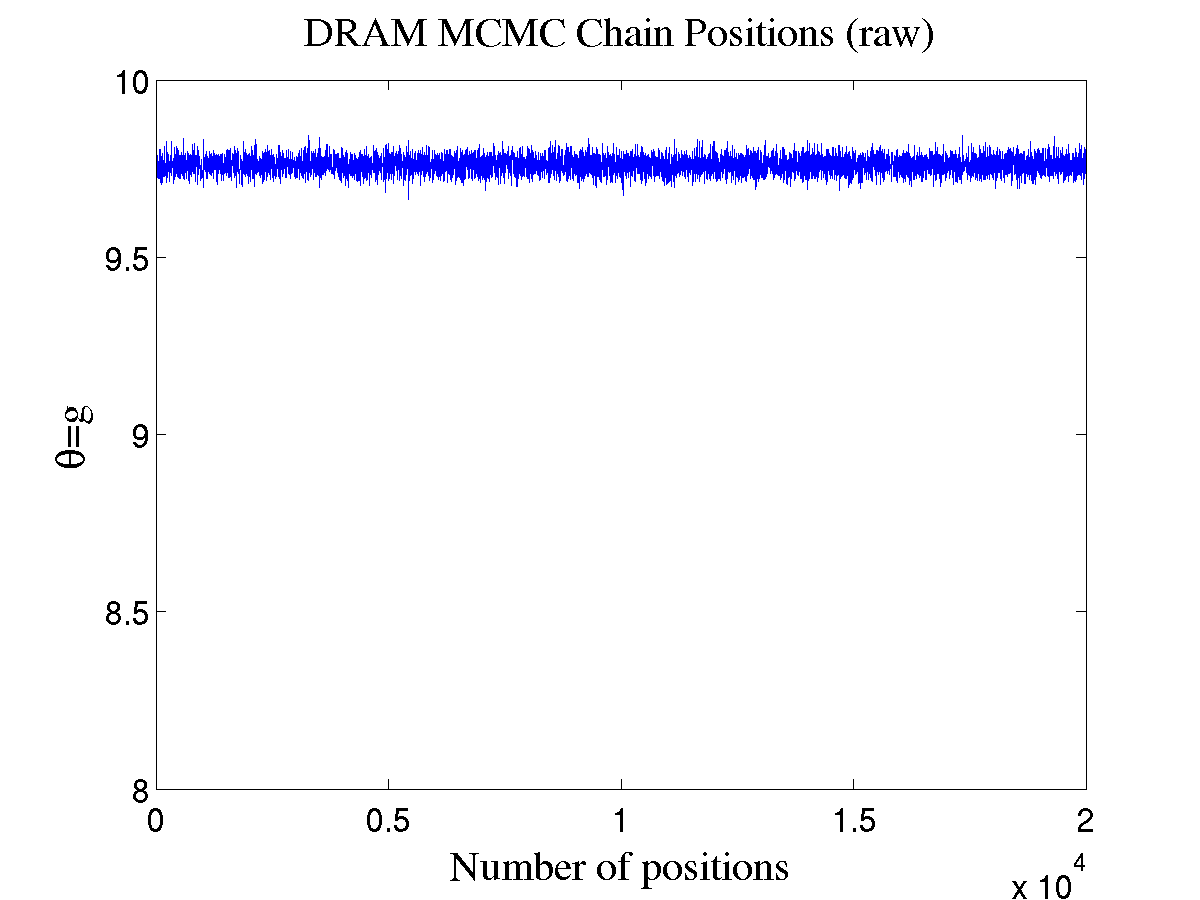
\includegraphics[scale=0.35]{figs/sip_gravity_chain_pos_raw.png}\label{fig:sip_gravity_chain_pos_raw}}
\subfigure[Filtered chain]{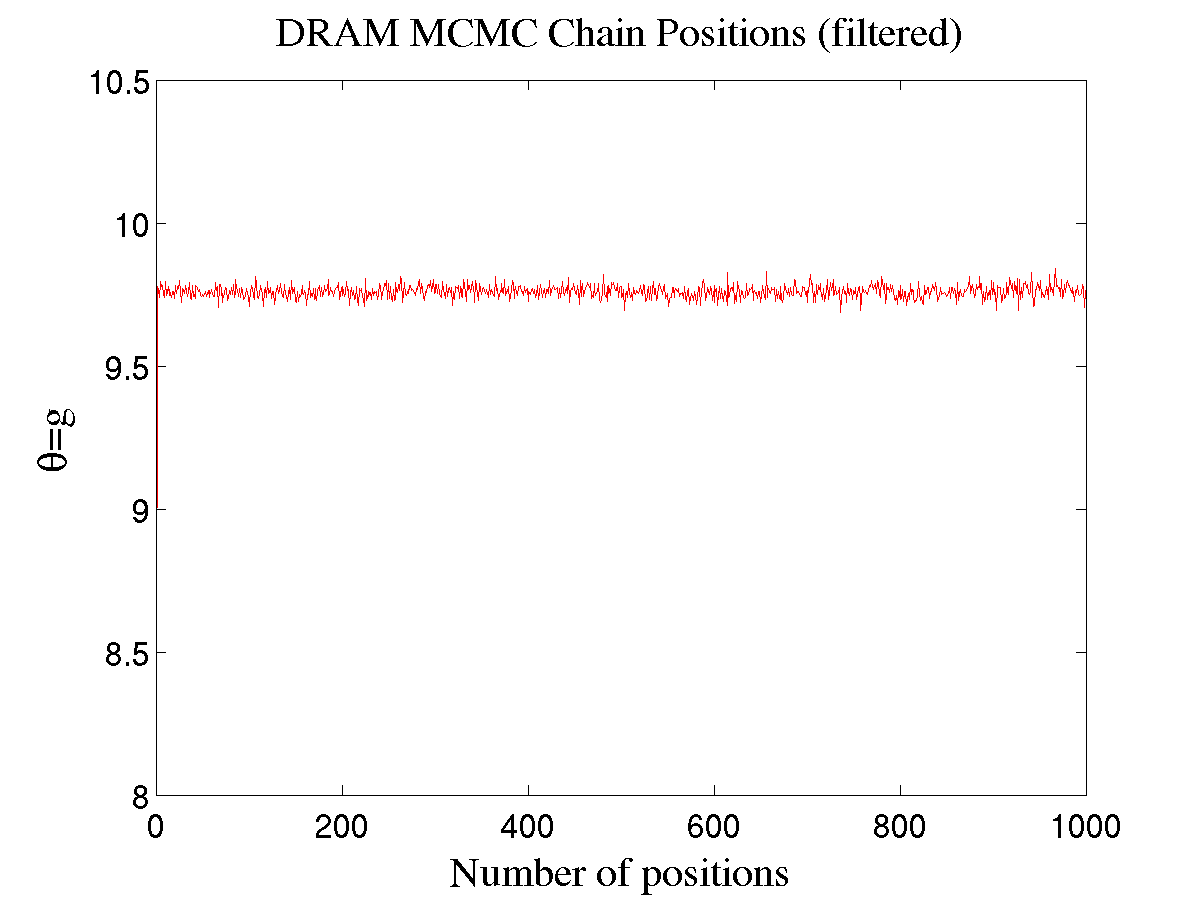
\includegraphics[scale=0.35]{figs/sip_gravity_chain_pos_filt.png}\label{fig:sip_gravity_chain_pos_filtered}}
\vspace*{-10pt}
\caption{MCMC raw chain with \chainsizeresults{} positions and a filtered chain with lag of 20 positions.}
\end{figure}

\paragraph{Histogram Plots}\

In order to plot histograms of the parameter using either the raw chain or the filtered chain, you simply have to use the pre-defined Matlab function \verb+hist+.
%The Matlab code presented in Listing \ref{matlab:hist} below shows how to create the Figure \ref{fig:sip_gravity_hist_raw};
%once more, Figure \ref{fig:sip_gravity_hist_filtered} is obtained by making suitable adjustments on that code.
%
\begin{lstlisting}[label=matlab:hist,caption={Matlab code for the histogram plot.}]
% inside Matlab
>> sip_gravity_raw_chain
>> nbins=100;
>> hist(ip_mh_rawChain_unified,nbins)
>> title('Parameter Histogram (raw chain)','fontsize',20);
>> xlabel('Gravity (m/s^2)','fontsize',20);
>> ylabel('Frequency','fontsize',20);
>> grid on;
\end{lstlisting}

\begin{figure}[htb]
\centering 
\subfigure[Raw chain]{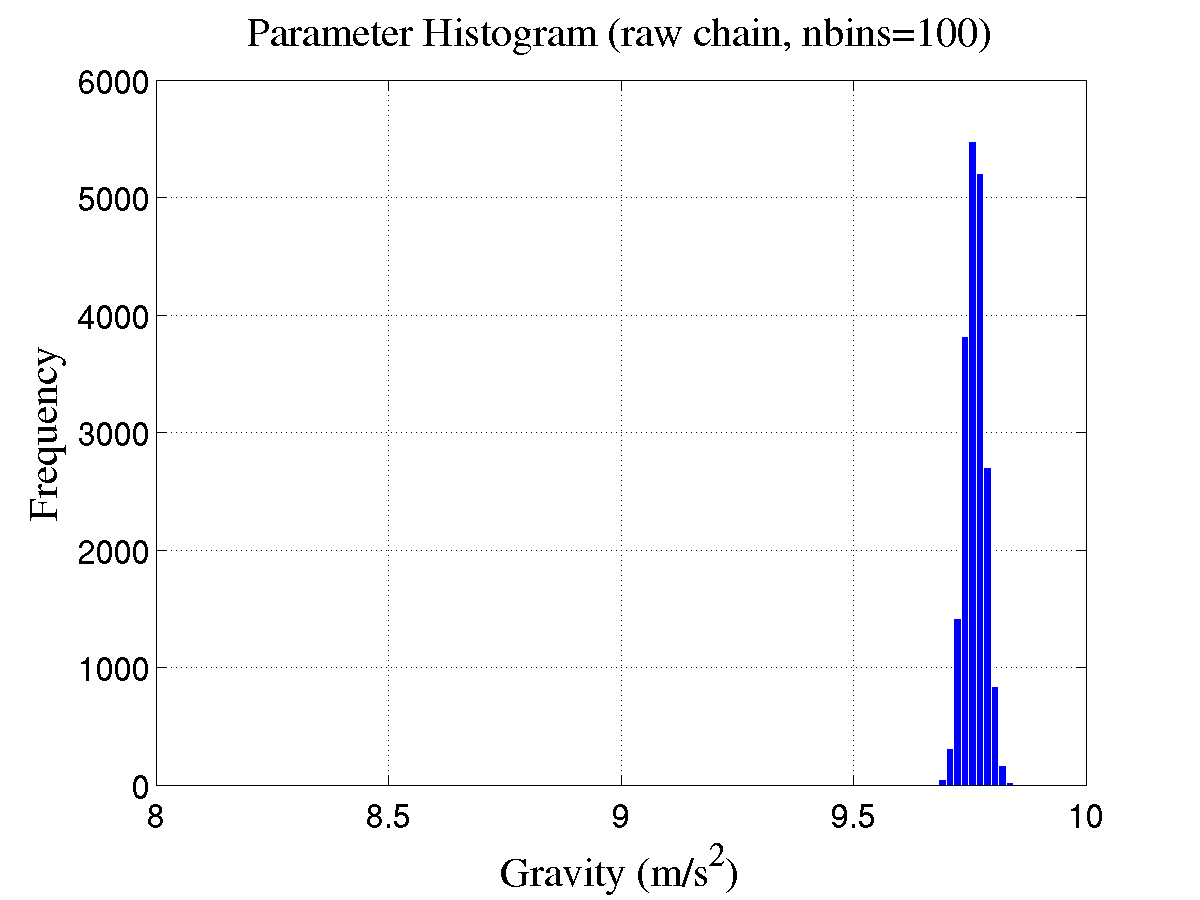
\includegraphics[scale=0.35]{figs/sip_gravity_hist_raw.png}\label{fig:sip_gravity_hist_raw}}
\subfigure[Filtered chain]{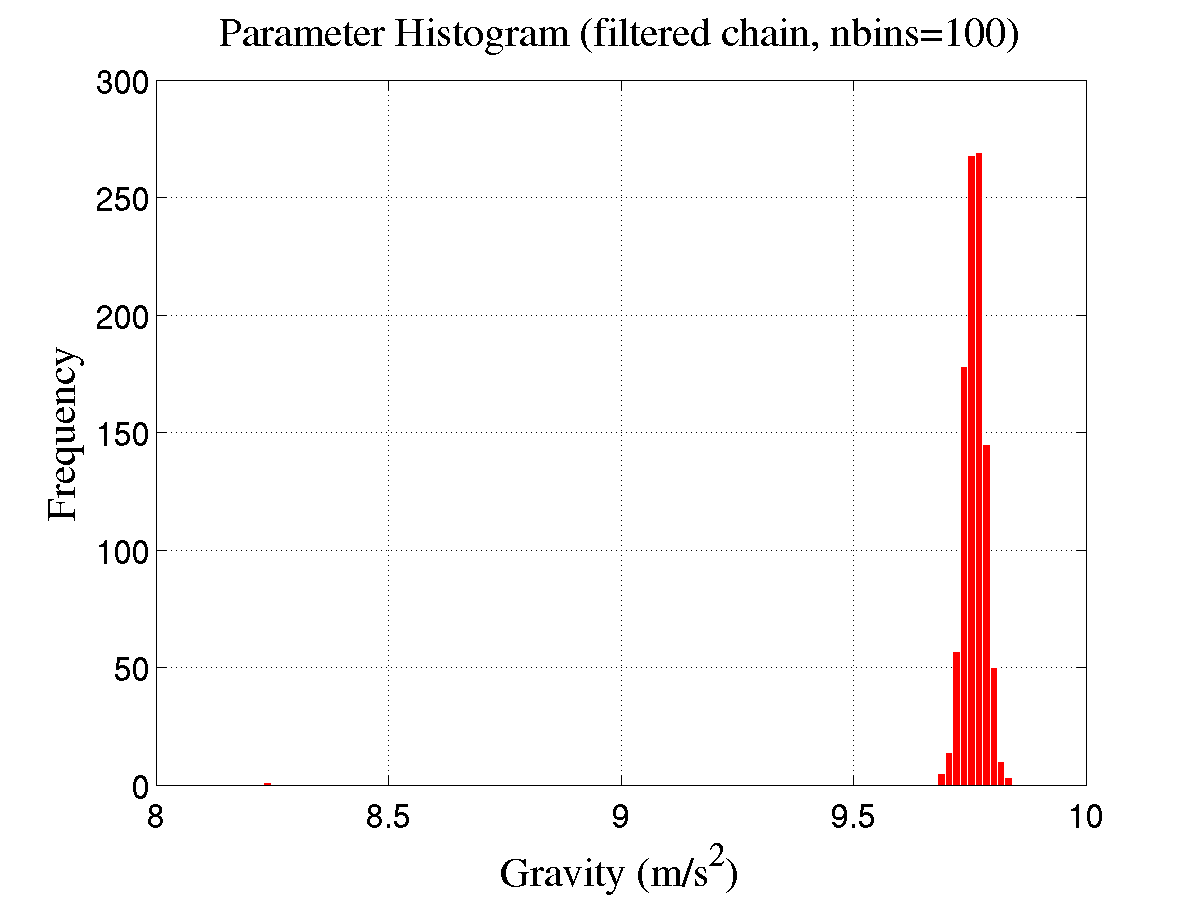
\includegraphics[scale=0.35]{figs/sip_gravity_hist_filt.png}\label{fig:sip_gravity_hist_filtered}}
\vspace*{-10pt}
\caption{Histograms of parameter $\theta=g$. }
\end{figure}

\paragraph{KDE Plots} \

Matlab function \verb+ksdensity+ (Kernel smoothing density estimate) together with the option \verb+'pdf'+ may be used for plotting the KDE of the parameter.
\begin{lstlisting}[label=matlab:kde,caption={Matlab code for the KDE plot.}]
% inside Matlab
>> sip_gravity_raw_chain
>> [f,xi] = ksdensity(ip_mh_rawChain_unified,'function','pdf');
>> plot(xi,f,'-b','linewidth',3)
>> title('Parameter Kernel Density Estimation','fontsize',20);
>> xlabel('Gravity (m/s^2)','fontsize',20);
>> ylabel('KDE','fontsize',20);
>> grid on;
\end{lstlisting}

%Figure \ref{fig:sip_gravity_kde_raw} is created by using Matlab commands presented in Listing \ref{matlab:kde} above.
\begin{figure}[htpb]
\centering 
\subfigure[Raw chain]{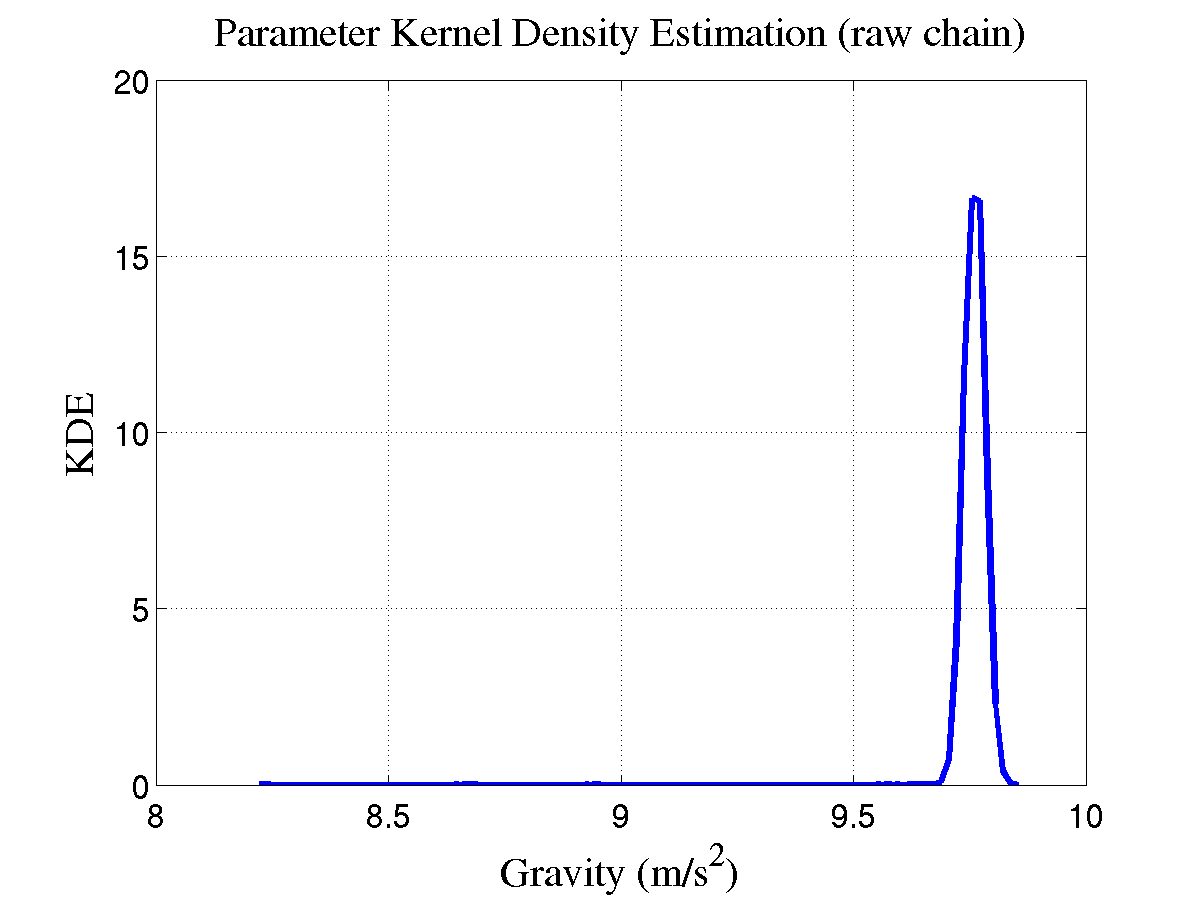
\includegraphics[scale=0.35]{figs/sip_gravity_kde_raw.png}\label{fig:sip_gravity_kde_raw}}
\subfigure[Filtered chain]{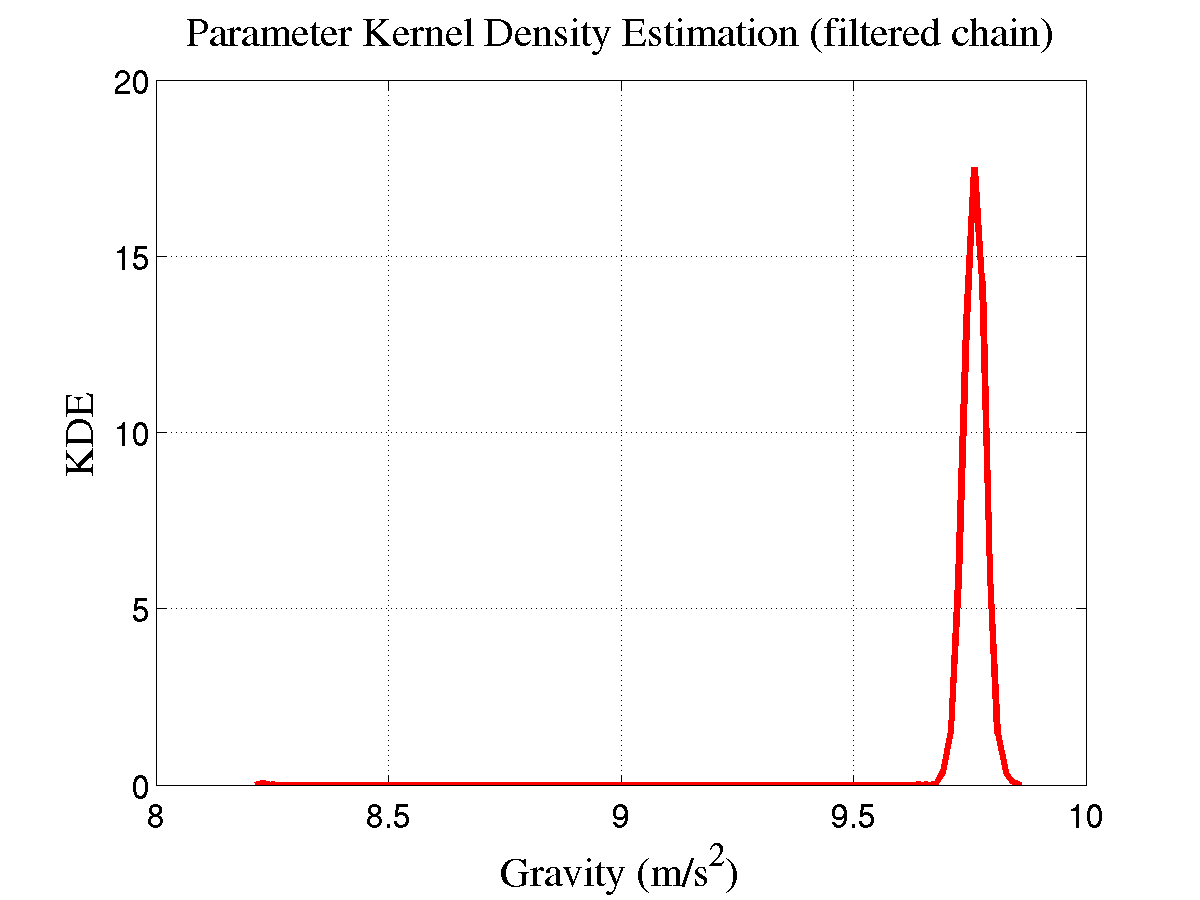
\includegraphics[scale=0.35]{figs/sip_gravity_kde_filt.png}\label{fig:sip_gravity_kde_filtered}}
\vspace*{-10pt}
\caption{Kernel Density Estimation. }
\end{figure}


% \subsubsection{Checking a KDE Plot Against Brute-Force Plot of the Likelihood Function}
% 
% See Figure \ref{fig:sip_gravity_compare_brute_force_unnormal}.
% %Figures \ref{fig:sip_gravity_compare_brute_force_unnormal} and \ref{fig:sip_gravity_compare_brute_force_normal} depict unnormalized and normalized KDE distributions
% %comparing the solution of the SIP provided by QUESO ($\pi_{\text{post}} (g)$) and the analytical (brute force) distribution.
% 
% \begin{figure}[htpb]
% \centering 
% %\subfigure[Unnormalized]{\includegraphics[scale=0.35]{figs/gravity_likelihood_brute_force_compare_post_pdf_0.png}\label{fig:sip_gravity_compare_brute_force_unnormal}}
% %\subfigure[Normalized]{\includegraphics[scale=0.35]{figs/gravity_likelihood_brute_force_compare_post_pdf_normalized0.png}\label{fig:sip_gravity_compare_brute_force_normal}}
% \subfigure{\includegraphics[scale=0.35]{figs/gravity_likelihood_brute_force_compare_post_pdf_0.png}\label{fig:sip_gravity_compare_brute_force_unnormal}}
% \vspace*{-10pt}
% \caption{Comparison of the posterior KDE for $g$ against the brute force calculation of the likelihood on a regular grid on $g$.
% }
% \end{figure}
% 
% %The code had to be slightly modified in order to replace QUESO sampling from the uniform distribution for the gravity with what we call a `brute force sampling'.
% %This brute force `sampling'  consists of recovering a pre-defined amount of values for $g$ from an equally spaced interval.
% %This is accomplished in lines 75 -- 100 of code \ref{code:gravity_compute_bruteforce_C}: it replaces Steps 4-6 (lines 100-150)
% %of the original application code provided in Algorithm \ref{code:gravity_compute_C}.
% 
% %\lstinputlisting[caption={Application code modified to `brute force' sampling from pre-defined interval.}, label={code:gravity_compute_bruteforce_C},  linerange={28-1000}]{../../brute_force/gravity_compute.C}
%  
% %Once more, Matlab function \verb+ksdensity+ (Kernel smoothing density estimate) may be used for plotting the KDE of the parameter.
% %The Matlab code below is responsible for the generation of Figure \ref{fig:sip_gravity_compare_brute_force_unnormal}.
% %Note that it reads the file \verb+gravity_likeli_brute_force.dat+, which is an output of the brute force code depicted in Listing \ref{code:gravity_compute_bruteforce_C}.
% %%
% %\begin{lstlisting}[label=matlab:kde_bruteforce,caption={Matlab code for the comparison of KDE plot from QUESO and `brute force'.}]
% %% inside Matlab
% %>> [g,like]=textread('gravity_likeli_brute_force.dat', '%f %f' );
% %>> [f,xi] = ksdensity(ip_mh_rawChain_unified,'function','pdf');
% %>> [haxes,hline1,hline2] = plotyy(xi,f,g,exp(like),'plot', 'plot');
% %>> axes(haxes(1));
% %>> ylabel('\pi_{post}(g) - QUESO/raw chain','fontname', 'Times', 'fontsize',20);
% %>> axes(haxes(2));
% %>> ylabel('\pi_{like}(g) -  brute force','fontname', 'Times', 'fontsize',20);
% %>> grid on;
% %>> title('Unnormalized distributions','fontname', 'Times', 'fontsize',20);
% %>> set(hline1,'linewidth',3);
% %>> set(hline2,'linewidth',3);
% %\end{lstlisting}


\paragraph{CDF Plots} \

Matlab function \verb+ksdensity+ (Kernel smoothing density estimate) with \verb+'cdf'+ option may also be used for plotting the Cumulative Distribution Function of the parameter.


\begin{lstlisting}[label=matlab:cdf,caption={Matlab code for the CDF plot.}]
% inside Matlab
>> sip_gravity_raw_chain
>> [f,xi] = ksdensity(ip_mh_rawChain_unified,'function','cdf');
>> plot(xi,f,'-b','linewidth',3)
>> title('Parameter Cumulative Distribution Function','fontsize',20);
>> xlabel('Gravity (m/s^2)','fontsize',20);
>> ylabel('CDF','fontsize',20);
>> grid on;
\end{lstlisting}

%Similarly, Figure \ref{fig:sip_gravity_cdf_raw} is created by using above Matlab commands.
\begin{figure}[ht]
\centering 
\subfigure[Raw chain]{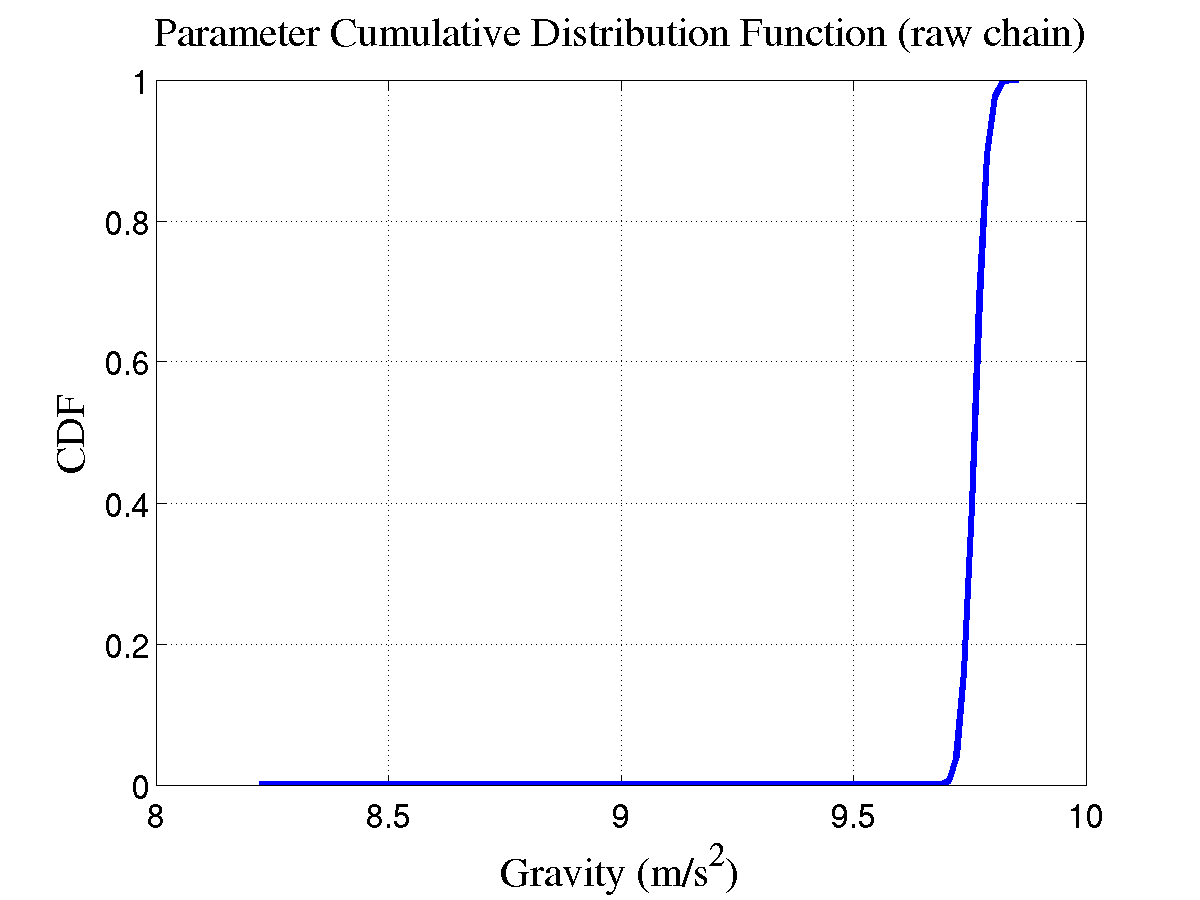
\includegraphics[scale=0.35]{figs/sip_gravity_cdf_raw.png}\label{fig:sip_gravity_cdf_raw}}
\subfigure[Filtered chain]{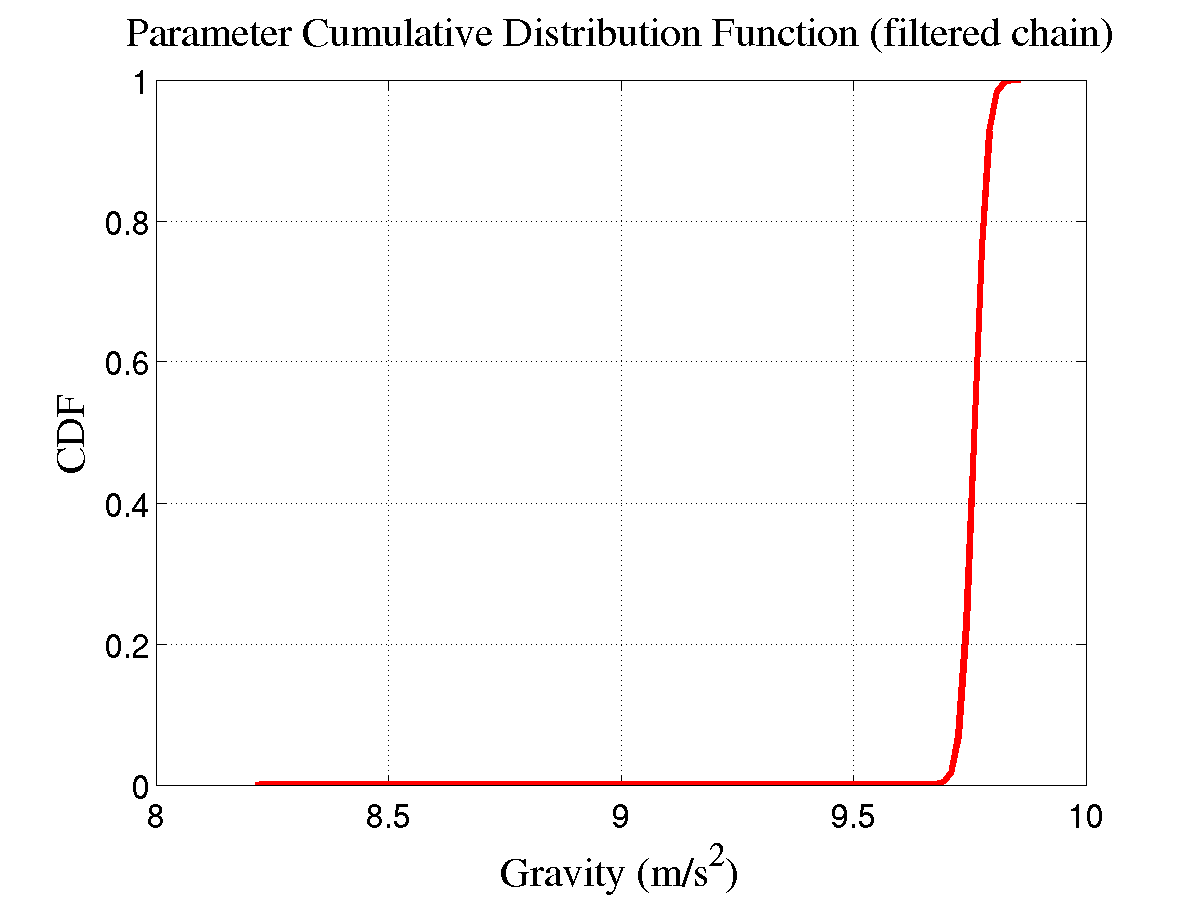
\includegraphics[scale=0.35]{figs/sip_gravity_cdf_filt.png}\label{fig:sip_gravity_cdf_filtered}}
\vspace*{-10pt}
\caption{Cumulative Distribution Function. }
\end{figure}

\paragraph{Autocorrelation Plots}\

The code presented in Listing \ref{matlab:autocorr} uses matlab function \verb+autocorr+ to generate Figure \ref{fig:sip_gravity_autocorrelation_raw_filt}
which presents the autocorrelation of the parameter $g$ in both cases: raw and filtered chain.

\begin{lstlisting}[label=matlab:autocorr,caption={Matlab code for the autocorrelation plots.}]
% inside Matlab
>> sip_gravity_raw_chain
>> sip_gravity_filtered_chain
>> nlags=10;
>> [ACF_raw,lags,bounds]= autocorr(ip_mh_rawChain_unified, nlags, 0);
>> [ACF_filt,lags,bounds]=autocorr(ip_mh_filtChain_unified,nlags, 0);
>> plot(lags,ACF_raw,'bo-',lags,ACF_filt,'r*-','linewidth',3);
>> ylabel('Autocorrelation for \theta=g','fontsize',20);
>> xlabel('Lag','fontsize',20);
>> title('Parameter Autocorrelation','fontsize',20);
>> grid on;
>> h=legend('raw chain','filtered chain','location','northeast');
>> set(h,'fontsize',16);
\end{lstlisting}

\begin{figure}[htpb]
\centering
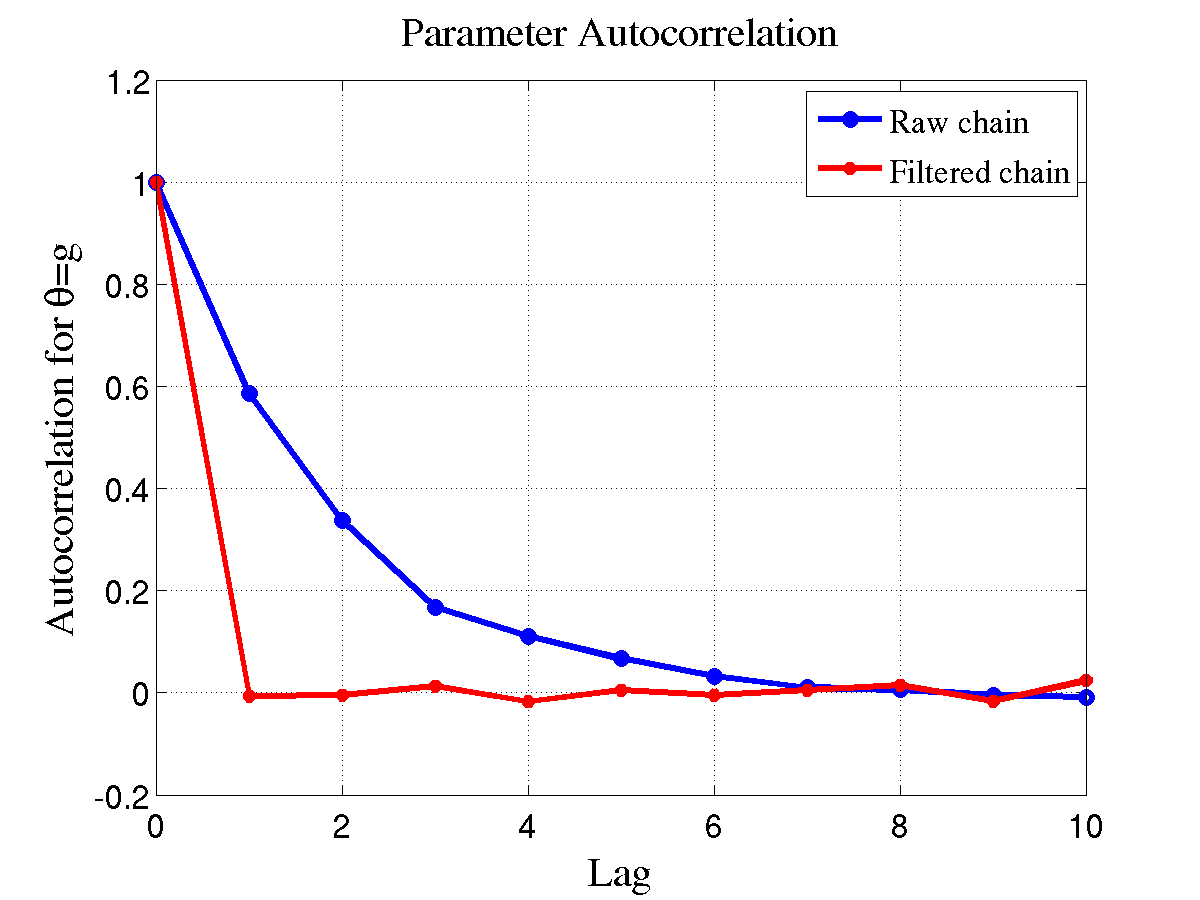
\includegraphics[scale=0.35]{figs/sip_gravity_autocorrelation_raw_filt.png}
\vspace{-8pt}
\caption{
Autocorrelation plots. }
\label{fig:sip_gravity_autocorrelation_raw_filt}
\end{figure}

\paragraph{Covariance and Correlation Matrices}\

Matlab function \verb+cov+ calculates the covariance matrix for a data matrix (where each column represents a separate quantity), and \verb+corr+ calculates the correlation matrix.
Since our statistical inverse problem has only one parameter (the acceleration $g$ due to gravity), both covariance and correlation matrices have dimension $1 \times 1$, i.e., they are scalars.

\begin{lstlisting}[label=matlab:cov_matrix,caption={Matlab code for finding the covariance matrix.}]
% inside Matlab
>> sip_gravity_raw_chain;
>> cov_matrix_g = cov(ip_mh_rawChain_unified)
   
cov_matrix_g =

   6.8709e-04
>> corr_matrix_g = corr(ip_mh_rawChain_unified)

corr_matrix_g =

     1
>>
\end{lstlisting}


\subsubsection{Statistical Forward Problem}


\paragraph{Chain Plots} \

It is quite simple to plot, using Matlab, the chain of positions generated by the Monte Carlo algorithm implemented within QUESO and called during the solution of the statistical forward problem. 
%The sequence of Matlab commands presented in Listing \ref{matlab:chain_qoi} generates the graphic depicted in Figure~\ref{fig:sfp_gravity_chain}. 

\begin{lstlisting}[label=matlab:chain_qoi,caption={Matlab code for the chain plot.}]
% inside Matlab
>> sfp_gravity_qoi_seq.m
>> plot(fp_mc_QoiSeq_unified);
>> ylabel('QoI','fontsize',20);
>> xlabel('Number of positions','fontsize',20);
>> title('MC Chain Positions','fontsize',20);
\end{lstlisting}

\begin{figure}[htb]
\centering 
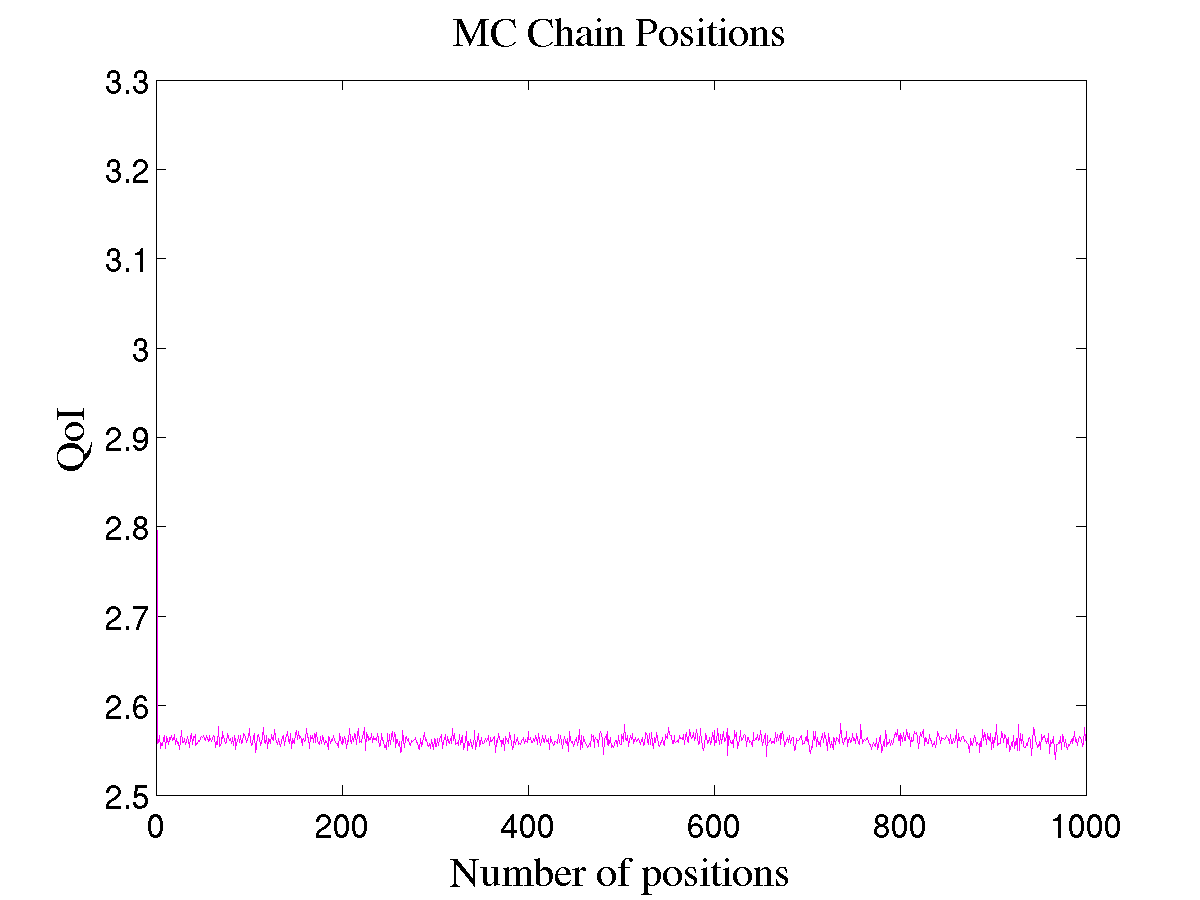
\includegraphics[scale=0.35]{figs/sfp_gravity_chain_pos.png}
\vspace*{-10pt}
\caption{MC chain positions for the QoI.}
\label{fig:sfp_gravity_chain}
\end{figure}

\paragraph{Histogram Plots} \

In order to plot a histogram of the QoI, you may use the pre-defined Matlab function \verb+hist+.
%The Matlab code presented in Listing \ref{matlab:hist_qoi} below shows how to create the Figure~\ref{fig:sfp_gravity_hist}.
%
\begin{lstlisting}[label=matlab:hist_qoi,caption={Matlab code for the QoI histogram plot.}]
>> sfp_gravity_qoi_seq.m
>> nbins=100;
>> hist(fp_mc_QoiSeq_unified);
>> title('QoI Histogram','fontsize',20);
>> xlabel('Distance traveled (m)','fontsize',20);
>> ylabel('Frequency','fontsize',20);
>> grid on;
\end{lstlisting}

\begin{figure}[htb]
\centering 
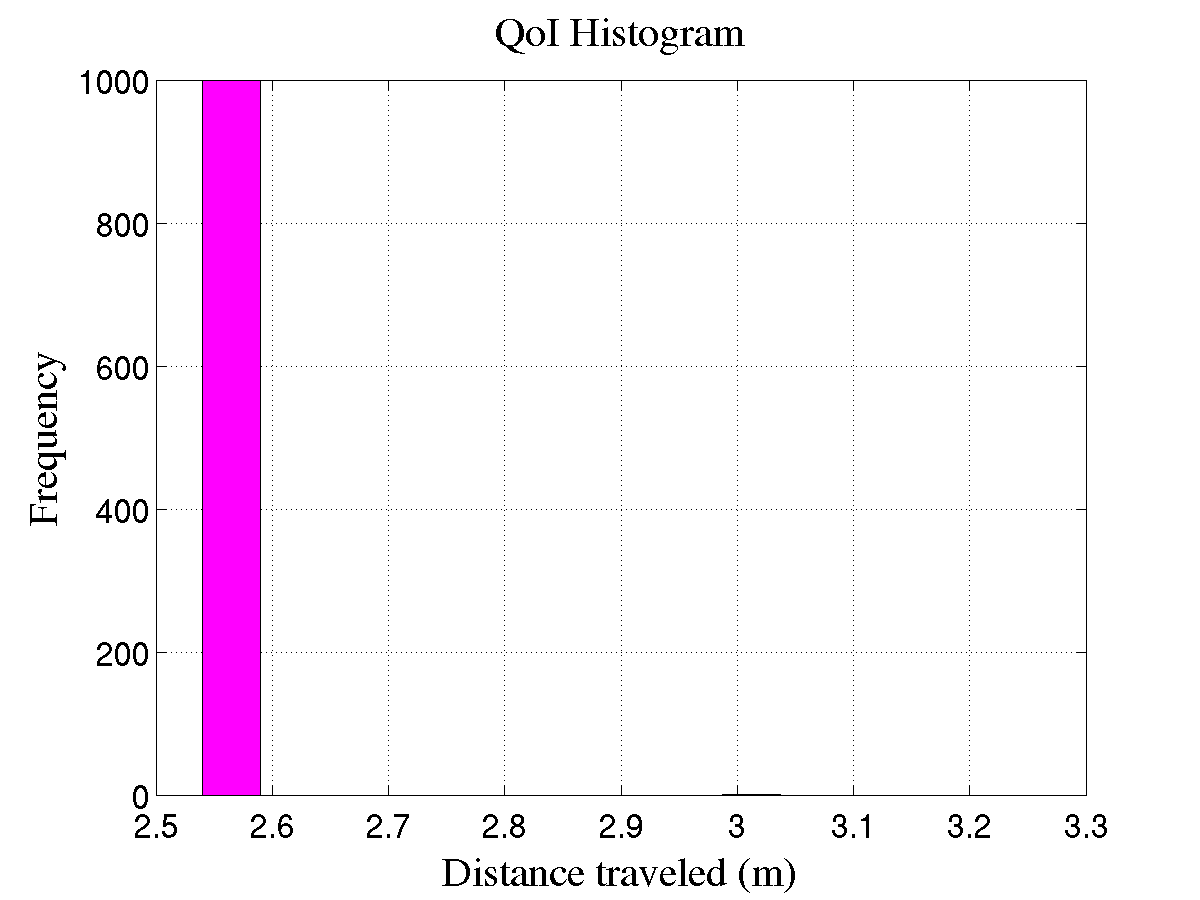
\includegraphics[scale=0.35]{figs/sfp_gravity_hist.png}
\vspace{-10pt}
\caption{Histogram of QoI $=d$.}
\label{fig:sfp_gravity_hist}
\end{figure}

\paragraph{KDE Plots} \

Matlab function \verb+ksdensity+ (Kernel smoothing density estimate) together with the option \verb+'pdf'+ may be used for plotting the KDE of the he QoI.
\begin{lstlisting}[label=matlab:kde_qoi,caption={Matlab code for the QoI KDE plot.}]
% inside Matlab
>> sfp_gravity_qoi_seq.m
>> [f,xi] = ksdensity(fp_mc_QoiSeq_unified,'function','pdf');
>> plot(xi,f,'-b','linewidth',3)
>> title('QoI Kernel Density Estimation ','fontsize',20);
>> xlabel('Distance traveled (m)','fontsize',20);
>> ylabel('KDE','fontsize',20);
>> grid on;
\end{lstlisting}

\begin{figure}[p]
\centering 
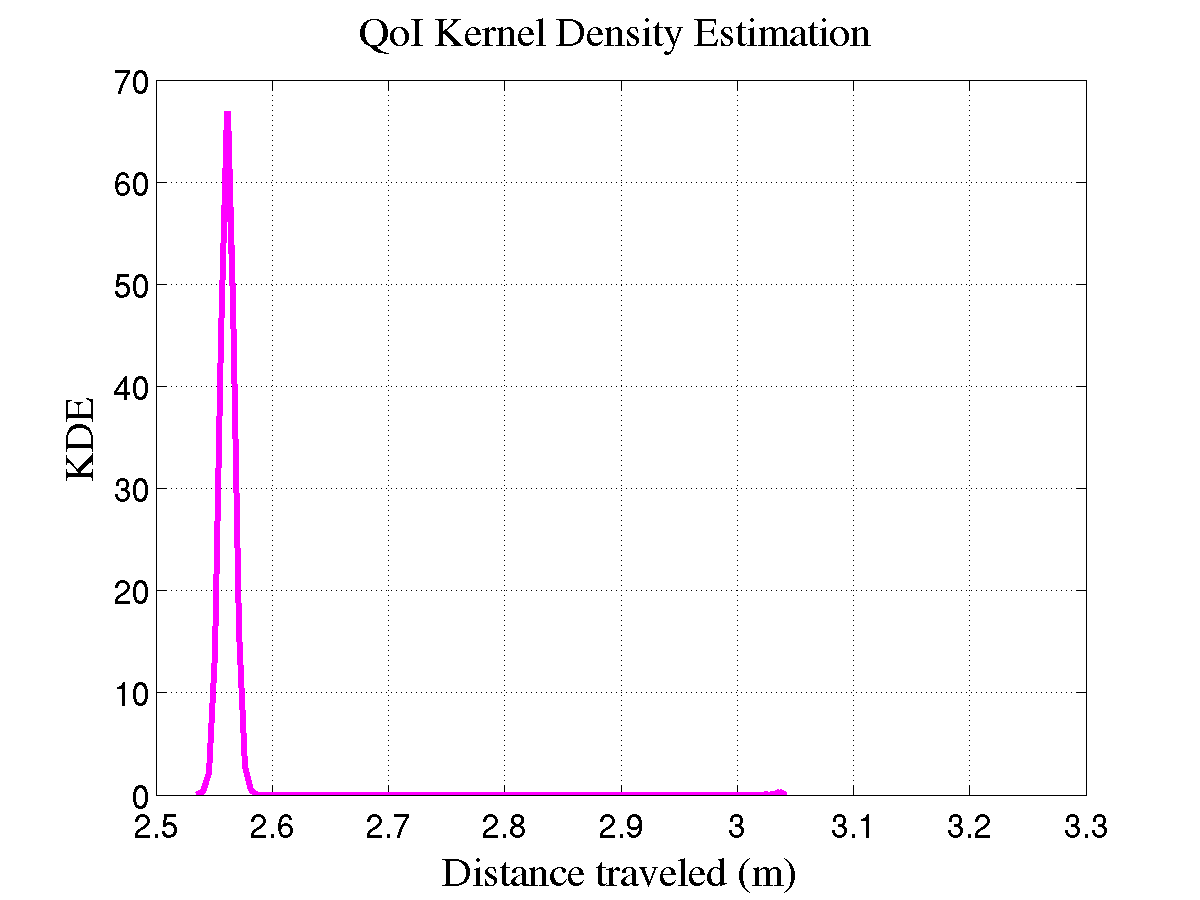
\includegraphics[scale=0.35]{figs/sfp_gravity_kde.png}
\vspace*{-10pt}
\caption{Kernel Density Estimation.}
\label{fig:sfp_gravity_kde}
\end{figure}

\paragraph{CDF Plots} \

Matlab function \verb+ksdensity+ (Kernel smoothing density estimate) with \verb+'cdf'+ option may also be used for plotting the Cumulative Distribution Function of the QoI.

\begin{lstlisting}[label=matlab:cdf_qoi,caption={Matlab code for the QoI CDF plot.}]
% inside Matlab
>> sfp_gravity_qoi_seq.m
>> [f,xi] = ksdensity(fp_mc_QoiSeq_unified,'function','cdf');
>> plot(xi,f,'-b','linewidth',3)
>> title('QoI Cumulative Distribution Function ','fontsize',20);
>> xlabel('Distance traveled (m)','fontsize',20);
>> ylabel('CDF','fontsize',20);
>> grid on;
\end{lstlisting}

\begin{figure}[p]
\centering 
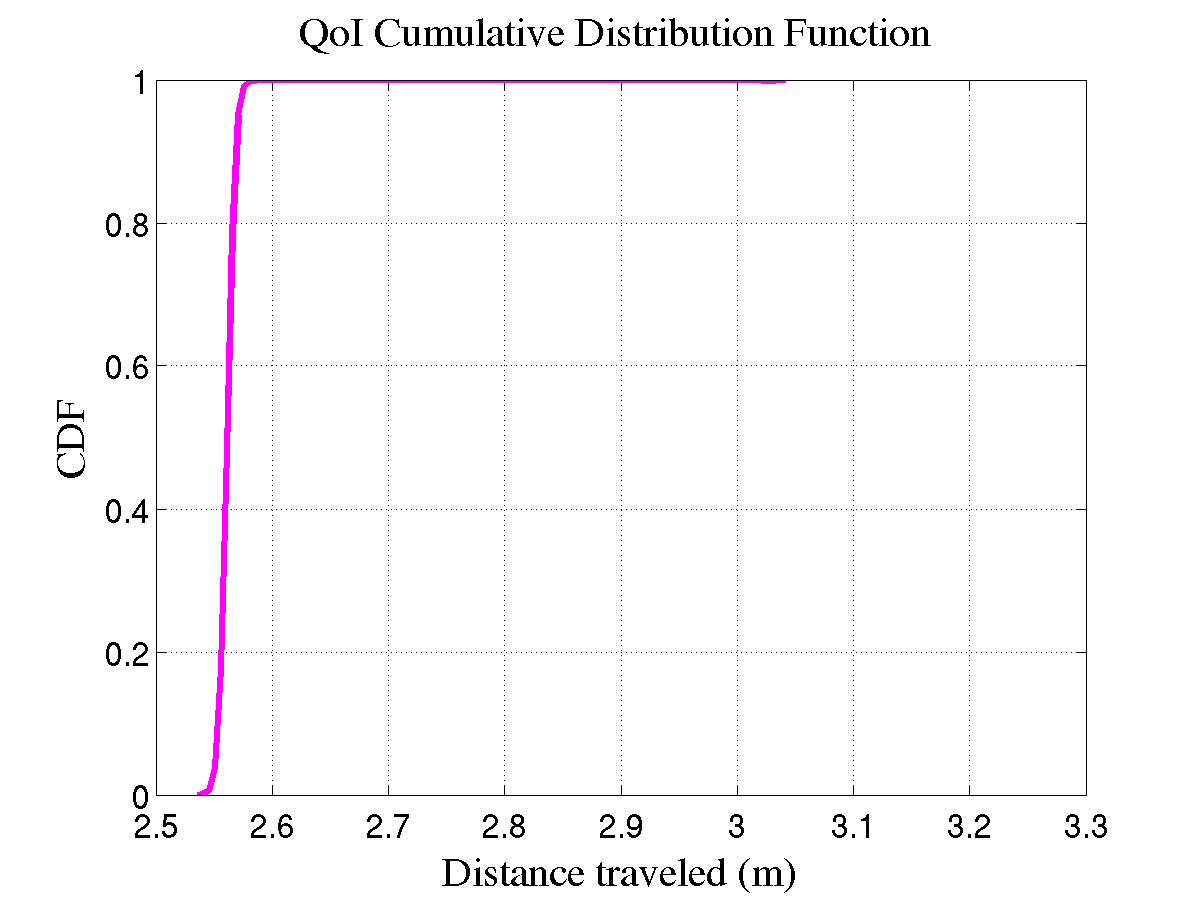
\includegraphics[scale=0.35]{figs/sfp_gravity_cdf.png}
\vspace*{-10pt}
\caption{Cumulative Distribution Function.}
\label{fig:sfp_gravity_cdf}
\end{figure}

\paragraph{Autocorrelation Plots} \

The code presented in Listing \ref{matlab:autocorr_qoi} uses Matlab function \verb+autocorr+ to generate Figure \ref{fig:sfp_gravity_autocorrelation},
which presents the autocorrelation of the QoI $d$.

\begin{lstlisting}[label=matlab:autocorr_qoi,caption={Matlab code for the QoI autocorrelation plot.}]
% inside Matlab
>> sfp_gravity_qoi_seq.m
>> nlags=10;
>> [ACF, lags, bounds] = autocorr(fp_mc_QoiSeq_unified, nlags, 0);
>> plot(lags,ACF,'bo-','linewidth',3);
>> ylabel('Autocorrelation for QoI = d','fontsize',20);
>> xlabel('Lag','fontsize',20);
>> title('QoI Autocorrelation','fontsize',20);
>> grid on;
\end{lstlisting}

\begin{figure}[p]
\centering
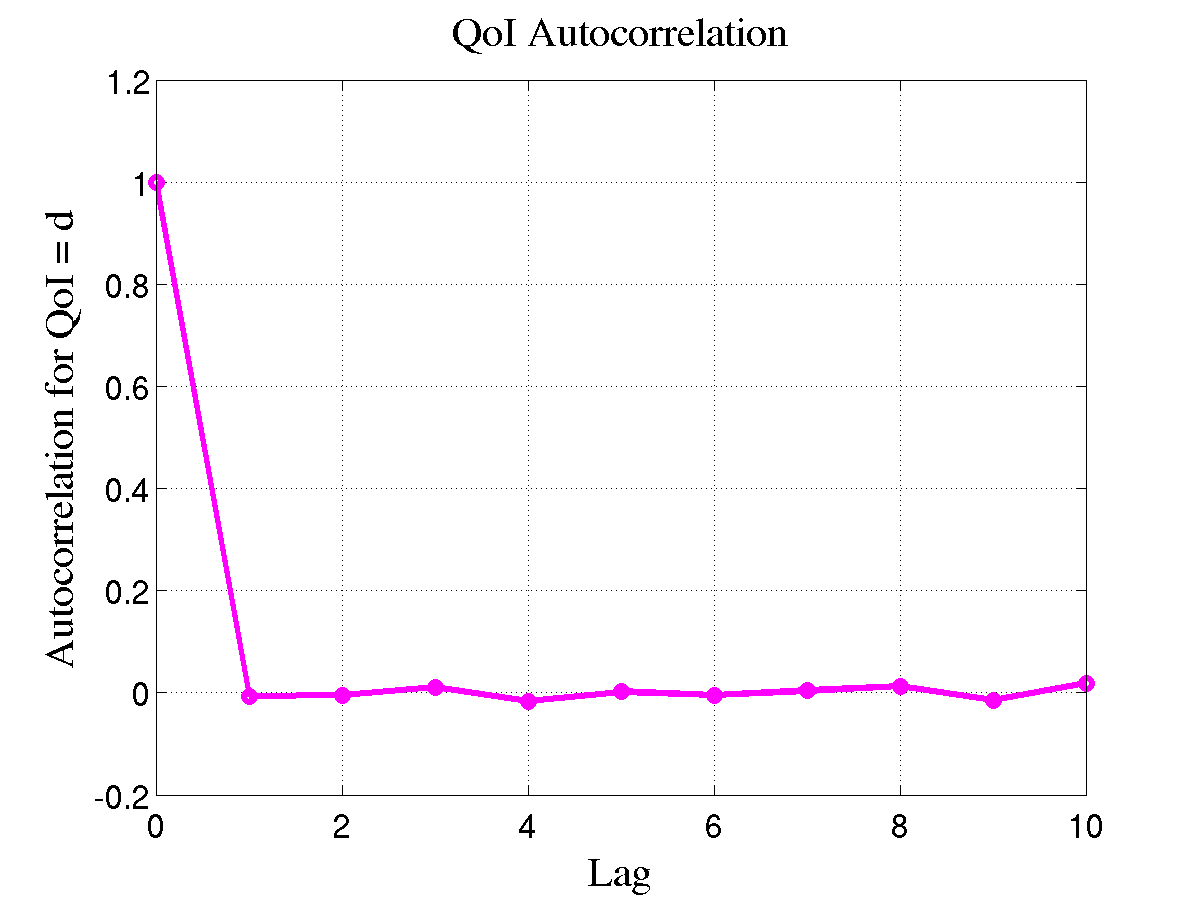
\includegraphics[scale=0.35]{figs/sfp_gravity_autocorrelation.png}
\vspace*{-10pt}
\caption{Autocorrelation plot.}
\label{fig:sfp_gravity_autocorrelation}
\end{figure}

\paragraph{Covariance and Correlation Matrices} \

For a matrix input \verb+X+, where each row is an observation, and each column is a variable, the Matlab function \verb+cov(X)+ may be used to calculate the covariance matrix.
%The command \verb+diag(cov(X))+ is a vector of variances for each column, and, therefore, \verb+sqrt(diag(cov(X)))+ is a vector of standard deviations.  

Thus,  in order to calculated the covariance matrix between the parameter and the quantity of interest sequences generated by Monte Carlo sampler with QUESO,
one may simply define \verb+X=[fp_mc_ParamSeq_unified fp_mc_QoiSeq_unified]+.
The code presented in Listing \ref{matlab:cov_pqoi} shows the usage of Matlab commands for finding such the matrix.

\begin{lstlisting}[label=matlab:cov_pqoi,caption={Matlab code for the matrix of covariance between parameter $g$ and QoI $d$.}]
% inside Matlab
>> sfp_gravity_qoi_seq;
>> sfp_gravity_p_seq;
>> X=[fp_mc_ParamSeq_unified fp_mc_QoiSeq_unified];
>> cov_p_QoI = cov(X)

cov_p_QoI =
	  [ 2.826e-03 	-8.555e-04 ] 
	  [-8.555e-04 	 2.599e-04 ]

\end{lstlisting}

Analogously, the Matlab function \verb+corrcoef(X)+ returns a matrix of correlation coefficients calculated from an input matrix \verb+X+ whose rows are observations and whose columns are variables.
In order to calculated the correlation matrix between the parameter and the QoI sequences, one may simply define \verb+X=[fp_mc_ParamSeq_unified fp_mc_QoiSeq_unified]+.
% The matrix R = corrcoef(X) is related to the covariance matrix C = cov(X) b

\begin{lstlisting}[label=matlab:corr_param_qoi,caption={Matlab code for the matrix of correlation between parameter $g$ and quantity of interest $d$.}]
% inside Matlab
>> sfp_gravity_qoi_seq;
>> sfp_gravity_p_seq;
>> X=[fp_mc_ParamSeq_unified fp_mc_QoiSeq_unified];
>> corr_p_QoI = corrcoef(X)

corr_p_QoI =
	  [ 1.000e+00 	-9.981e-01 ] 
	  [-9.981e-01 	 1.000e+00 ]
>>
\end{lstlisting}




\section{\texttt{validationCycle}}\label{sec:example_tga}

This is the last and more complex of all \Queso{} examples. 
In this example, we numerically solve a statistical inverse problem related to a thermogravimetric experiment, where a material sample has its mass measured while loosing it through a controlled heating process. 

Given a simple mass evolution model that has a temperature profile and material
properties as input parameters, and given thermogravimetric measurements with
prescribed variances, the statistical inverse problems ask for the
specification of the random variables that represent the unknown material
properties. We compute probability density functions with the Bayesian approach
and compute sets of realizations through the Metropolis-Hastings algorithm with
delayed rejection.
% DRAM Markov chain algorithm.
%Once the random variables are computed, they become input parameters on statistical forward problems,
%which ask for the statistical prediction of the sample mass evolution under a specified temperature profile.
%We solve the statistical forward problems with the Monte Carlo algorithm.

We qualitatively analyze the sensitivity of the solutions with respect to
problem characteristics, namely ``amount'' of data and ``quality'' of data, and
also with respect to algorithm options, namely chain initial position, number
of delayed rejections
%, covariance matrix adaptivity
and chain size.




\subsection{Thermogravimetric Experiments and a Simple Model}

Suppose a given material sample of initial mass $m_0$ and at initial temperature $T_0$ is heated with constant heating rate $\beta$ (K/min). Heating is maintained until the sample fully ablates (decomposes). The sample mass $m(T)$ is measured at temperatures $T>T_0$.
Let $w(T)~=~m(T)/m_0$ denote the mass fraction.

% 
% A material sample with initial mass $m_0$ and at initial temperature $T_0$ is heated
% with constant heating rate $\beta$ (K/min) until it fully decomposes.
% Let $w(T)=m(T)/m_0$ denote the mass fraction.
\begin{figure}[!ht]
\centering
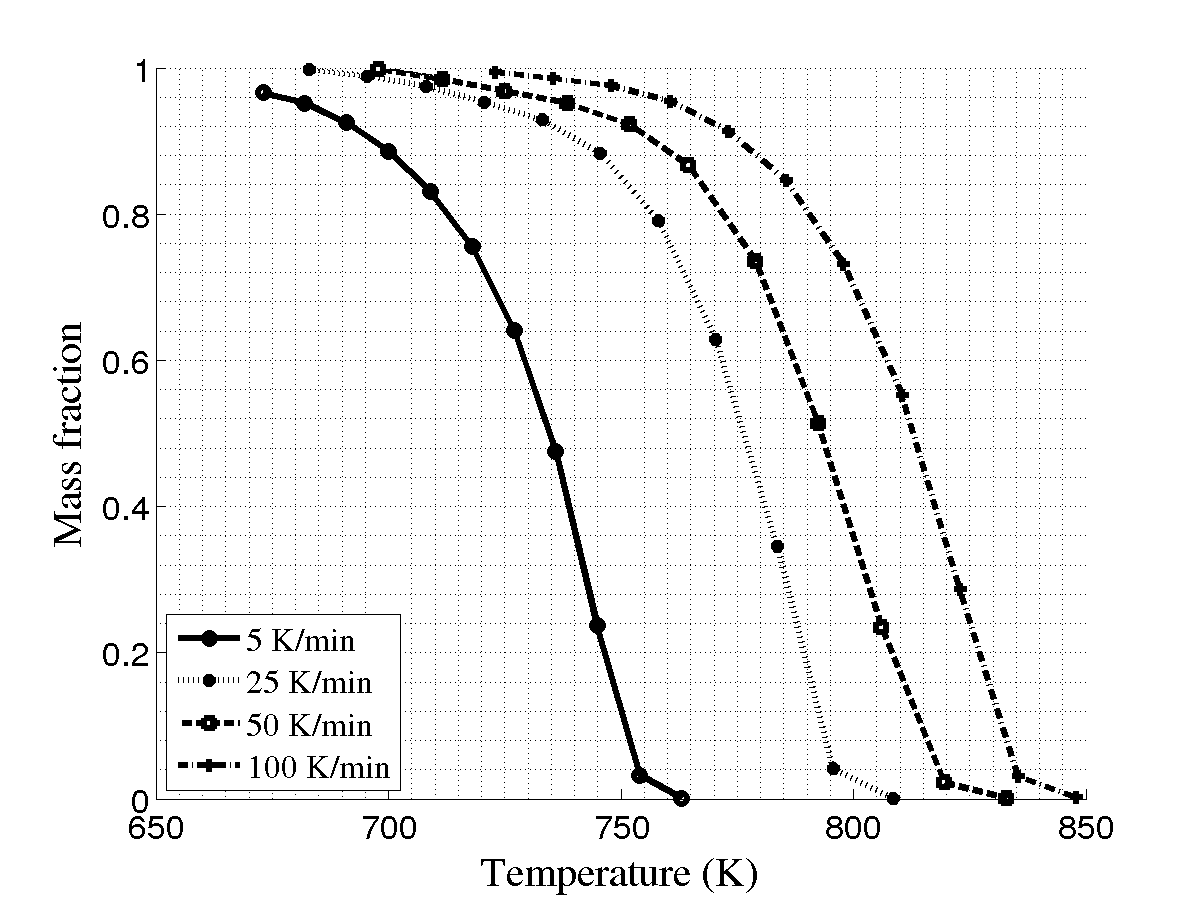
\includegraphics[scale=0.4]{figs/tga_experiment_data.png}
\vspace*{-8pt}
\caption{Mass fraction decay over temperature given different heating rates. Data from J. A. Conesa, R. F. Marcilla and J. A. Caballero, ``Thermogravimetric studies on the thermal decomposition of polyethylenes'', {\it J. Anal. Appl. Pyrolysis}, 36(1):1-15, 1996}
\label{fig:tga-exp-data}
\end{figure}


It is convenient to transform the kinetic equation to a \emph{per unit temperature}
form by dividing through by $\beta$. Thus, a simple approach to
the simulation of a thermogravimetric phenomenon consists on modeling the
sample as a homogeneous material of scalar properties $A>0$ and $E>0$ whose
relative mass $w$ obeys the following initial value ordinal differential
equation problem:
\begin{equation}\label{eq:tga-model}
\left\{
\begin{array}{rcll}
{\displaystyle \frac{dw}{dt} } & = & -\dfrac{A w}{\beta} \exp\left(-\frac{E}{RT}\right), & t \geqslant 0,\\
& & \\
w(0) & = & 1, &
\end{array}
\right.
\end{equation}
where the kinetic parameters $A$ and $E$ are referred to, respectively, as pre-exponential factor (min$^{-1}$) and activation energy (J/mol).


In this combined SIP--SFP, we  calibrate both model parameters $A$ and $E$ given the mathematical model in Equation \eqref{eq:tga-model} and experimental data (Section \ref{sec:tga-data}). Then the inferred values for $A$ and $E$ are then used for uncertainty propagation on the remaining mass fraction at time $t=3.9$ s when $\beta=250$ K/min, i.e., our quantity of interest is $w(t=3.9)$. 

\subsection{Statistical Inverse Problem}\label{sec:tga-sip}

%
Let $\mathbf{m}=(A,E)$ be the vector of model parameters and $M=\mathbb{R}_{+}^{2}$ be the space of model parameters.
Let
$V_T$ denote the space of functions $f:\mathbb{R}_{+}\rightarrow\mathbb{R}_{+}$ that are weakly differentiable.
$V_T$ will be the space of temperature profiles.
Finally, let
$V_w$ denote the space of functions $f:\mathbb{R}_{+}\rightarrow[0,1]$ that are weakly differentiable.
$V_w$ will be the space of relative mass evolutions.
We will denote by
\begin{equation*}
w(\mathbf{m},T)\in V_w
\end{equation*}
the solution of Equation \eqref{eq:tga-model} for given $\mathbf{m}\in M$ and $T\in V_T$.


% 
% This model can be easily generalized to a sample composed of $N_{\text{mat}}\geqslant 1$ materials. We refer to \cite{eep_ices_rep1} for details.

\subsubsection{Misfit Functions $\mathcal{F}(\mathbf{m})$}

Let
$V_S$ denote the space of all functions $f:\mathbb{R}_{+}\rightarrow\mathbb{R}_{+}$ that are square-Lebesgue-integrable
over any finite interval.
$V_S$ will be the space of misfit weight functions.
Let
$V_{\sigma}$ denote the space of all functions $f:\mathbb{R}_{+}\rightarrow\mathbb{R}_+^{*}$ such that $1/f$ is square-Lebesgue-integrable
over any finite interval.
$V_{\sigma}$ will be the space of variance functions.

Given a reference relative mass evolution function $\text{$d$}\in V_w$,
a temperature profile $T\in V_T$,
and some $t_{_{\text{F}}}>0$,
let $\mathcal{F}:M\rightarrow\mathbb{R}$ be the functional defined by
\begin{equation*}
\mathcal{F}(\mathbf{m}) = \int_{0}^{t_{_{\text{F}}}}~\left\{[w(\mathbf{m},T)](t)-\text{$d$}(t)\right\}^2\cdot S(t)~dt,
\end{equation*}
or simply
\begin{equation}\label{eq-F}
\mathcal{F}(\mathbf{m}) = \int_{0}^{t_{_{\text{F}}}}~(w-d)^2\cdot S~dt.
\end{equation}


The functional \eqref{eq-F} is general enough for our studies, since it can properly describe
not only the case where one has continuous measurements $\text{$d$}$,
but also the case of a finite set of $N_{\text{meas}}$ discrete measurements $0\leqslant d_j\leqslant 1$,
$1\leqslant i\leqslant N_{\text{meas}}$ at instants $0\leqslant t_1 < t_2 < \ldots < t_{N_{\text{meas}}}$.

In the case of continuous measurements, for instance, one can set
\begin{equation*}
\mathcal{F}_1(\mathbf{m}) = \int_{0}^{t_{_{\text{F}}}}~\left\{[w(\mathbf{m},T)](t)-\text{$d$}(t)\right\}^2\cdot\frac{1}{\sigma^2(t)}~dt,
\end{equation*}
for some given variance function $\sigma^2\in V_S$ satisfying $\sigma(t)>0$ for all $t\geqslant 0$.

On the other hand, when measurements are discrete and a corresponding finite set of variances $\sigma_j^2>0,~j=1,2,\ldots,N_{\text{meas}}$ is given, one can set
\begin{equation*}
\mathcal{F}_2(\mathbf{m}) = \int_0^{t_{_F}}~\{[w(\mathbf{m},T)](t)-\hat{d}(t)\}^2\cdot\left[\sum_{j=1}^{N_{\text{meas}}}\frac{\delta(t-t_j)}{{\hat{\sigma}}^2(t)}\right]~dt,
\end{equation*}
where
$\hat{d}\in V_w$ and $\hat{\sigma}\in V_{\sigma}$ are any functions satisfying
$\hat{d}(t_j)=d_j$ and $\hat{\sigma}(t_j)=\sigma_j$, $j=1,2,\ldots,N_{\text{meas}}$,
in which case the functional simply becomes
\begin{equation*}
\mathcal{F}_2(\mathbf{m}) = \sum_{j=1}^{N_{\text{meas}}}~\frac{\{[w(\mathbf{m},T)](t_j)-d_j\}^2}{\sigma_j^2},
\end{equation*}
assuming, without loss of generality, that $t_{_F}\geqslant t_{N_{\text{meas}}}$.

\subsubsection{Bayesian Approach: Prior RV, Likelihood and Posterior RV}


In \underline{deterministic} inverse problems treat the unknown parameters as scalars or vectors and the goal is
the calculation of their best values according to a given criteria, usually least squares, e.g. solving the unconstrained optimization problem
\begin{equation}\label{eq-unconstrained-min}
\underset{\mathbf{m}\in M}{\text{min}}~\mathcal{F}(\mathbf{m}).
\end{equation}

In \underline{statistical} inverse problems, the unknown parameters are treated
as random variables (RVs) and the goal is the specification of their
probability density functions (PDFs)~\cite{KaSo05}.




Applying the Bayesian approach
\begin{equation*}
\pi_{\text{posterior}}(\mathbf{m})\propto \pi_{\text{prior}}(\mathbf{m})\cdot\pi_{\text{likelihood}}(\mathbf{m})
\end{equation*}
we have that for the TGA SIP, the prior distribution and the likelihood are, respectively:
\begin{equation*}
\pi_{\text{prior}}(\mathbf{m}) \propto e^{-\frac{1}{2}V(\mathbf{m})}\quad\text{and}\quad
%
\pi_{\text{likelihood}}(\mathbf{m}) \propto e^{-\frac{1}{2}\mathcal{F}(\mathbf{m})}.
\end{equation*}


Thus, we chose parameters $(A,E)$ to have joint uniform prior PDF over the open
square domain, i.e.:
$$\pi_{\text{prior}}=\mathcal{U}((1.0\times 10^{10},5.0\times 10^{11})\times (4.0\times 10^{5},6.0\times 10^{5})).$$



\subsubsection{Data from experiments}\label{sec:tga-data}

Table \ref{table:data-tga} presents the data collected in the TGA experiment. 

\begin{table}[htb]
\begin{center}
\begin{tabular}{cllc}
\toprule
Observation   & Temperature     & Relative mass             & Variance \\
index ``$i$'' & $T_i$ (K)       & $m^*_{\text{obs},i}$ (\%) & $V_i$    \\
\midrule
\midrule
 1            & $\quad$ 673.034 & $\quad$ 96.5855    & 0.1      \\
 2            & $\quad$ 682.003 & $\quad$ 95.1549    & 0.1      \\
 3            & $\quad$ 690.985 & $\quad$ 92.5048    & 0.1      \\
 4            & $\quad$ 699.979 & $\quad$ 88.6353    & 0.1      \\
 5            & $\quad$ 708.989 & $\quad$ 83.0585    & 0.1      \\
 6            & $\quad$ 718.02  & $\quad$ 75.5306    & 0.1      \\
 7            & $\quad$ 727.089 & $\quad$ 64.1003    & 0.1      \\
 8            & $\quad$ 735.96  & $\quad$ 47.5474    & 0.1      \\
 9            & $\quad$ 744.904 & $\quad$ 23.6777    & 0.1      \\
 10           & $\quad$ 754.062 & $\quad$ 03.2234    & 0.1      \\
 11           & $\quad$ 763.049 & $\quad$ 00.0855448 & 0.1      \\
\bottomrule
\end{tabular}
\vspace{-.2cm}
\caption{Experimental data.}\label{table:data-tga}
\end{center}
\end{table}

\subsection{Statistical Forward Problem}\label{sec:tga-sfp}

In spacecraft design, ablation is used to both cool and protect mechanical parts and/or payloads that would otherwise be damaged by extremely high temperatures. Two principal applications are heat shields for spacecraft entering a planetary atmosphere from space and cooling of rocket engine nozzles~\cite{wiki:ablation}. 

Suppose that an object about to re-enter the Earth atmosphere has a thermal
protection layer (shield) of composition of the same sample material described
in Section \ref{sec:tga-sip}. Also, as the object re-enters the atmosphere, its
shield loses mass according to Equation \eqref{eq:tga-model}.  The initial
sample temperature is $T_0=0.1$ K and it is then heated with constant rate
$\beta=5$ K/m.
% We are interested in answering a few questions:
% \begin{enumerate}
%  \item At scenario $\beta=250$ K/min, what is the remaining mass fraction at time $t=3.9$ s, i.e. $$w(t=3.9s)?$$
%  \item Supposing that a failure occurs when the remaining mass fraction is smaller than 20\%, what is the probability of failure at time $t=3.9$ s, i.e. $$P(w(t=3.9s)<0.2)?$$
%  \item  Supposing that the probability of failure is $\leq 5\%$, what is the margin in the prediction of the probability of failure?
% \end{enumerate}

We are interested in answering the following question: at scenario $\beta=250$
K/min, what is the remaining mass fraction at time $t=3.9$ s? In other words,
the quantity of interest is $w(t=3.9s)$.



% \todo{Suppose also that, under such conditions, our quantity of interest (QoI) is the time necessary to the sample to ablate 75\% of its mass, denoted by $t_\text{0.25}$ (s). In other words, we are interested in estimate how long it takes for $w=0.25$, or}
% \begin{equation}
%  \text{Find } t_\text{0.25} \text{ such as } w(t_\text{0.25} )=0.25
% \end{equation}

\subsubsection{The Input RV, QoI Function and Output RV}


The input random variables for this SFP are the inferred parameters $A$ and $E$ which are the solution (posterior PDF) of the inverse problem described in Section \ref{sec:tga-sip}. The output random variable for this example is the remaining mass fraction at 3.9 s, i.e. $w(t=3.9)$. Note that, since there is uncertainty in the parameters $A$ and $E$ (both given as PDFs), one can expect that this uncertainty will be propagated to $w(t=3.9)$, which will also be given as a PDF. Finally, the QoI function for $w$ is the solution of the Equation \eqref{eq:tga-model} evaluated when $t=3.9$ s, which is calculated using numerical integration with adjustable and acceptable time-stepping using GSL function \verb+gsl_odeiv_evolve_apply+\footnote{\url{http://www.gnu.org/software/gsl/manual/html_node/Evolution.html\#index-gsl_005fodeiv2_005fevolve_005fapply}}. 

\subsection{Running the Example}\label{sec:tga-run}

To run the executable provided (available after QUESO installation), and generate figures for the chains, PDFs, CDFs, etc., enter the following commands:
\begin{lstlisting}[label={},caption={}]
$ cd $HOME/LIBRARIES/QUESO-0.50.0/examples/validationCycle
$ rm outputData/*
$ ./exTgaValidationCycle_gsl tagCycle.inp    
$ matlab
   $ tga_cycle_plot.m     # inside matlab
   $ exit                 # inside matlab
$ ls -l outputData/*.png
  cal_parameter1_prior.png                cal_parameter2_prior.png                
  cal_val_parameter1_PDF.png              cal_val_parameter2_PDF.png              
  cal_val_parameter1_CDF.png              cal_val_parameter2_CDF.png              
  cal_val_parameter1_autocorr.png         cal_val_parameter2_autocorr.png
  cal_val_QoI_CDF.png                     cal_val_QoI_PDF.png
  cal_val_QoI_autocorrelation.png            
\end{lstlisting}
% cal_val_QoI_CDF_model_confidence_full.png
% cal_val_QoI_CDF_model_confidence_zoom.png


As a result, the user should have created several of PNG figures containing marginal posterior PDF, chain positions of the parameters and the QoI, histogram, cumulative density distribution and autocorrelation. The name of the figure files have been chosen to be informative, as shown in the Listing above.



\subsection{TGA Example Code}\label{sec:code-tga}



The program example given in this paper is compatible with version 0.47.1 of QUESO.
The source code for the example is composed of 5 files:
 \texttt{exTgaValidationCycle\_gsl.C} (Listing \ref{code:tga-main-c}),
 \texttt{exTgaValidationCycle\_appl.h} (Listing \ref{code:tga-appl-h}), 
 \texttt{exTgaValidationCycle\_likelihood.h}  (Listing \ref{code:tga-like-h}) and 
\texttt{exTgaValidationCycle\_qoi.C} (Listing \ref{code:tga-qoi-h}).



\lstinputlisting[caption=File \texttt{exTgaValidationCycle\_gsl.C}., label={code:tga-main-c}, linerange={28-1000}]{../../examples/validationCycle/src/exTgaValidationCycle_gsl.C}

\lstinputlisting[caption=File \texttt{exTgaValidationCycle\_appl.h}., label={code:tga-appl-h}, linerange={27-1000}]{../../examples/validationCycle/src/exTgaValidationCycle_appl.h}

\lstinputlisting[caption=File \texttt{exTgaValidationCycle\_likelihood.h.}, label={code:tga-like-h}, linerange={27-1000}]{../../examples/validationCycle/src/exTgaValidationCycle_likelihood.h}

\lstinputlisting[caption=File \texttt{exTgaValidationCycle\_qoi.h}., label={code:tga-qoi-h}, linerange={27-1000}]{../../examples/validationCycle/src/exTgaValidationCycle_qoi.h}




\subsection{Input File}\label{sec:tga-input-file}

The input file used with this TGA SIP--SFP QUESO provides QUESO with options
for its environments, and for both  MCMC and Monte-Carlo algorithms. It is
displayed in Listing~\ref{code:tga-input-file}.


\lstinputlisting[caption={File name \texttt{tgaCycle.inp} with options for QUESO library used in application code (Listings \ref{code:tga-main-c}-\ref{code:tga-like-h}})., 
label={code:tga-input-file},]{../../examples/validationCycle/tests/test_2012_11_15/tgaCycle.inp}



\subsection{Data Post-Processing and Visualization}\label{sec:tga-results}


According to the specifications of the input file in Listing~\ref{code:tga-input-file}, both a folder named \verb+outputData+ and a the following files should be generated:
\begin{verbatim}
file_cal_ip_raw.m        file_val_ip_raw.m        
file_cal_ip_raw_sub0.m   file_val_ip_raw_sub0.m
file_cal_fp_qoi2.m       file_val_fp_qoi2.m      
file_cal_fp_qoi2_sub0.m  file_val_fp_qoi2_sub0.m     
tgaCalOutput_sub0.m      tgaValOutput_sub0.m
display_sub0.txt    
\end{verbatim}


The sequence of Matlab commands is identical to the ones presented in Sections
\ref{sec:sip-results}, \ref{sec:sfp-results} and \ref{sec:gravity-results};
therefore, are omitted here. The reader is invited to explore the Matlab file
\texttt{tga\_cycle\_plot.m}  
%\texttt{validationCycle/tests/test\_2012\_11\_15/tga\_cycle\_plot.m} 
for details of how the figures have been generated.

\subsubsection{KDE Plots of Parameters}
Matlab function \verb+ksdensity+ (Kernel smoothing density estimate) together
with the option `\verb+pdf+' may be used to estimate the KDE of the parameters,
as illustrated in Figure \ref{fig:tga_ip_pdf}.
% \begin{figure}[htb]
% \centering 
% \subfloat{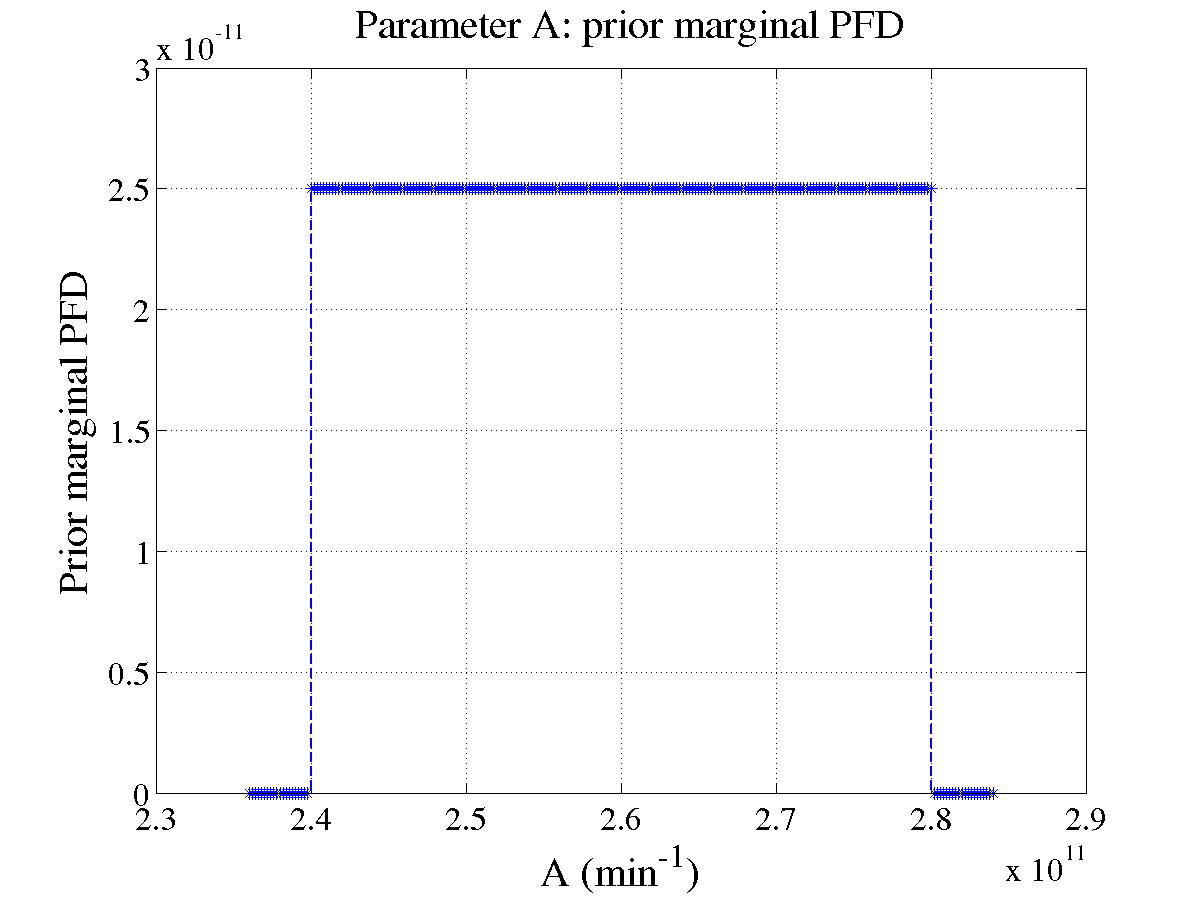
\includegraphics[scale=0.40]{figs/cal_parameter1_prior.png}}
% \subfloat{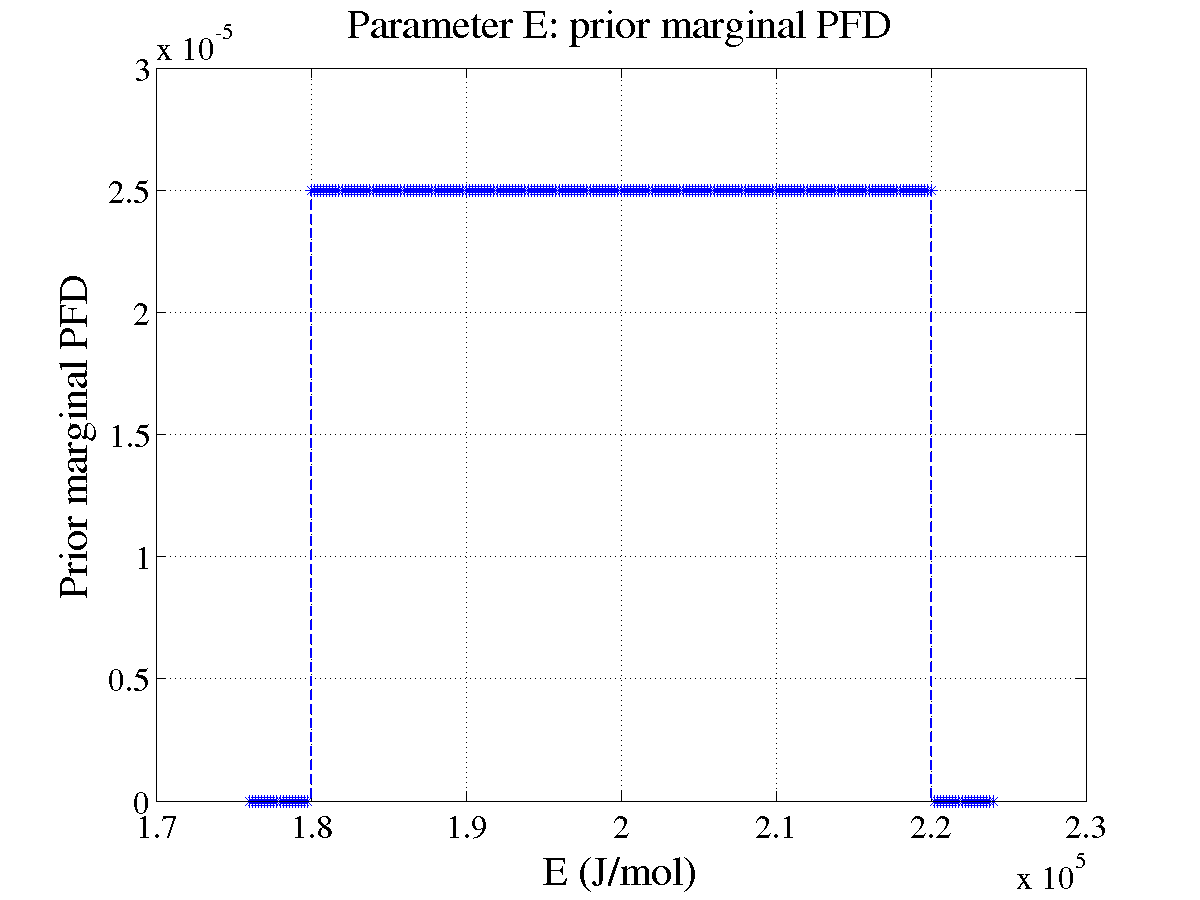
\includegraphics[scale=0.40]{figs/cal_parameter2_prior.png}}
% \vspace*{-10pt}
% \caption{Prior distributions of parameters $A$ and $E$.}
% \end{figure}
%
\begin{figure}[htpb]
\centering 
\subfloat{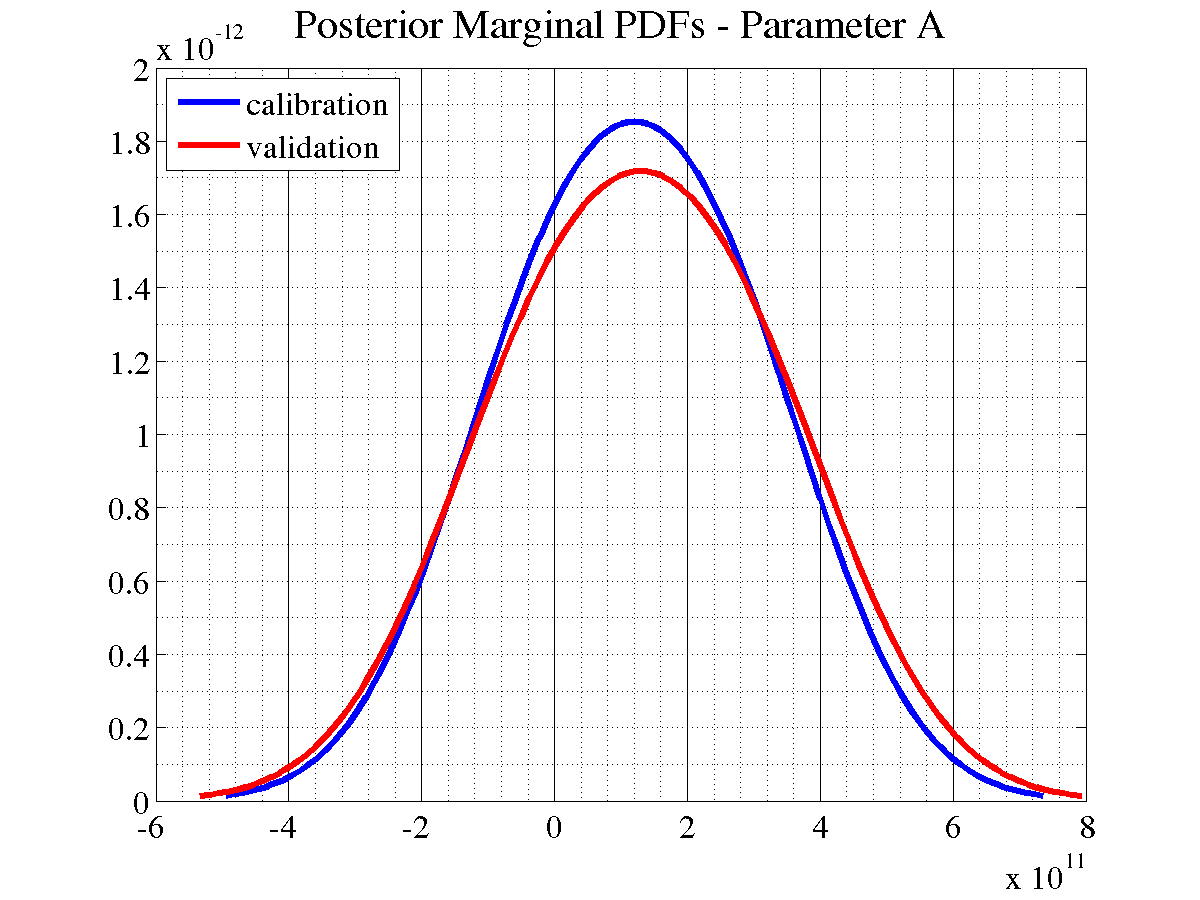
\includegraphics[scale=0.3]{figs/cal_val_parameter1_PDF.png}}
\subfloat{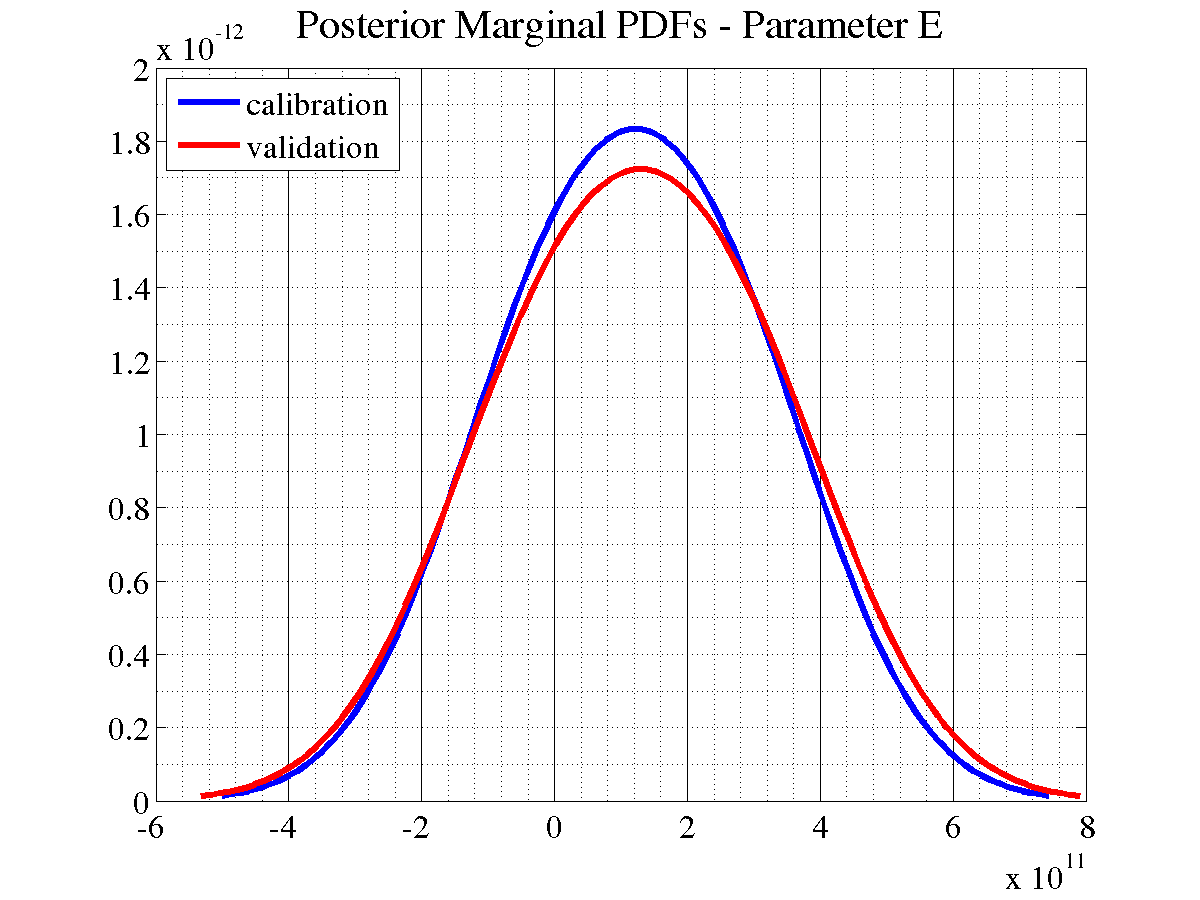
\includegraphics[scale=0.3]{figs/cal_val_parameter2_PDF.png}}
\vspace*{-10pt}
\caption{Posterior distributions of parameters $A$ and $E$.}
\label{fig:tga_ip_pdf}
\end{figure}



\subsubsection{CDF Plots of Parameters}

Matlab function \verb+ksdensity+ with \verb+'cdf'+ option may also be used for plotting the Cumulative Distribution Function of each one of the parameters, as illustrated in Figure \ref{fig:tga_ip_cdf}.
%
\begin{figure}[htpb]
\centering 
\subfloat{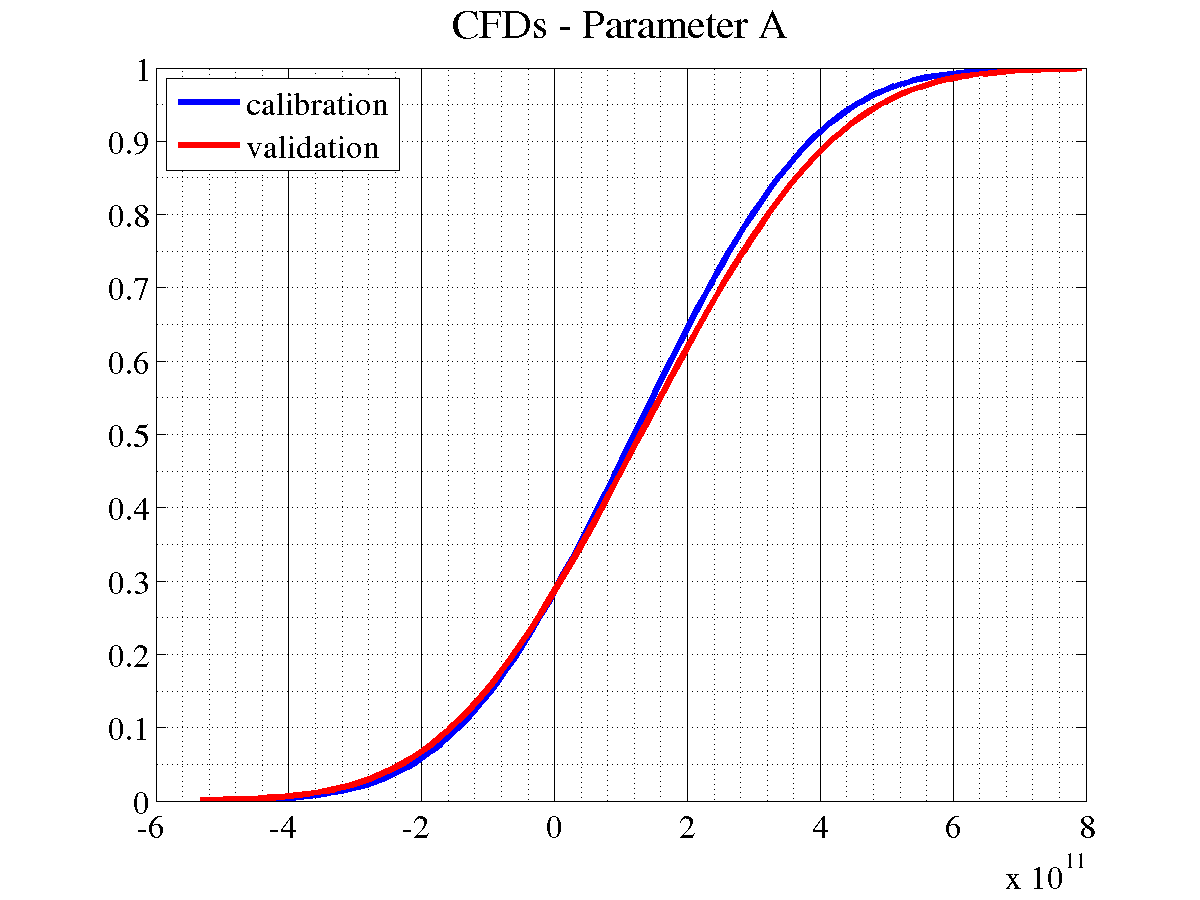
\includegraphics[scale=0.3]{figs/cal_val_parameter1_CDF.png}}
\subfloat{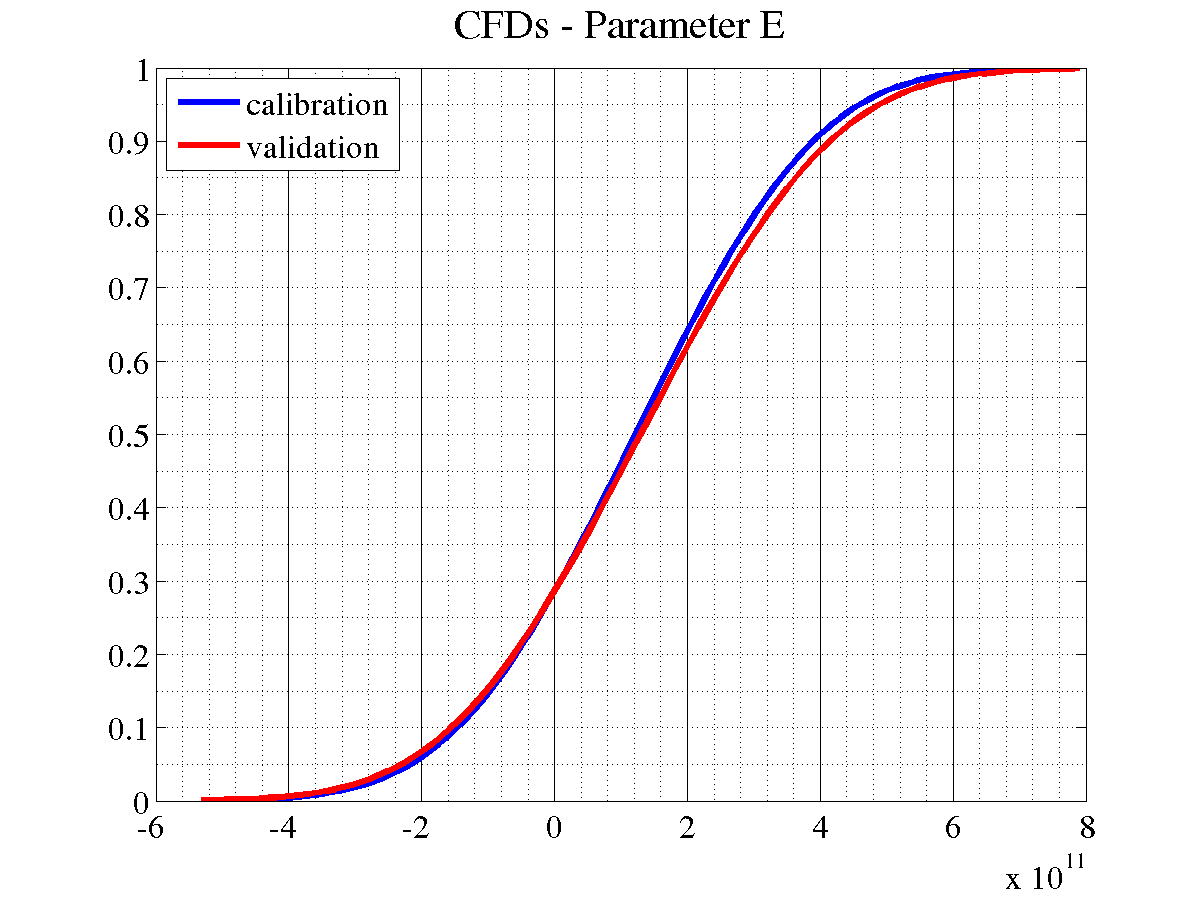
\includegraphics[scale=0.3]{figs/cal_val_parameter2_CDF.png}}
\vspace*{-10pt}
\caption{Cumulative density functions of parameters $A$ and $E$.}
\label{fig:tga_ip_cdf}
\end{figure}



\subsubsection{Autocorrelation Plots of Parameters}

Figure \ref{fig:tga_ip_autocorrelation_param} presents the autocorrelation of the parameters $A$ and $E$ in both cases: calibration and validation stages.

\begin{figure}[p]
\centering 
\subfloat{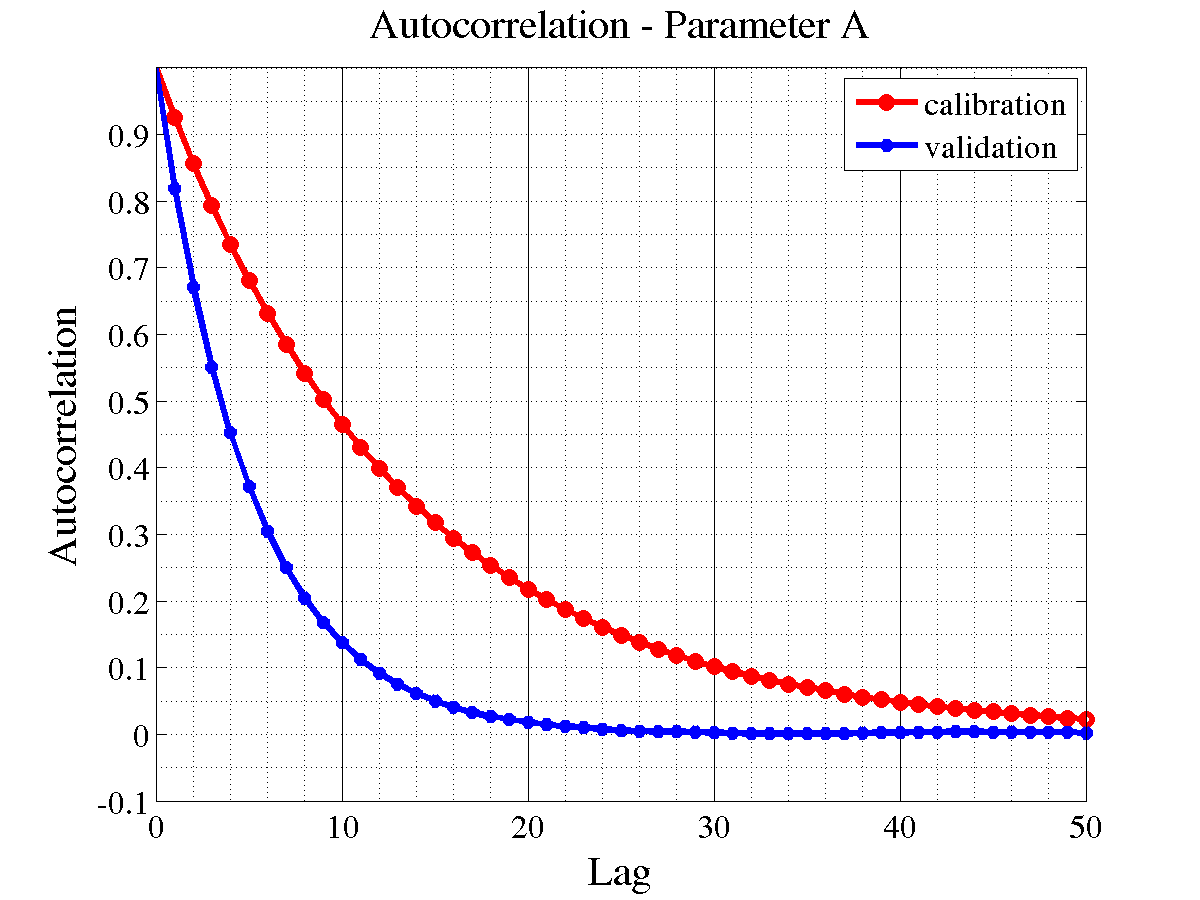
\includegraphics[scale=0.3]{figs/cal_val_parameter1_autocorrelation.png}}
\subfloat{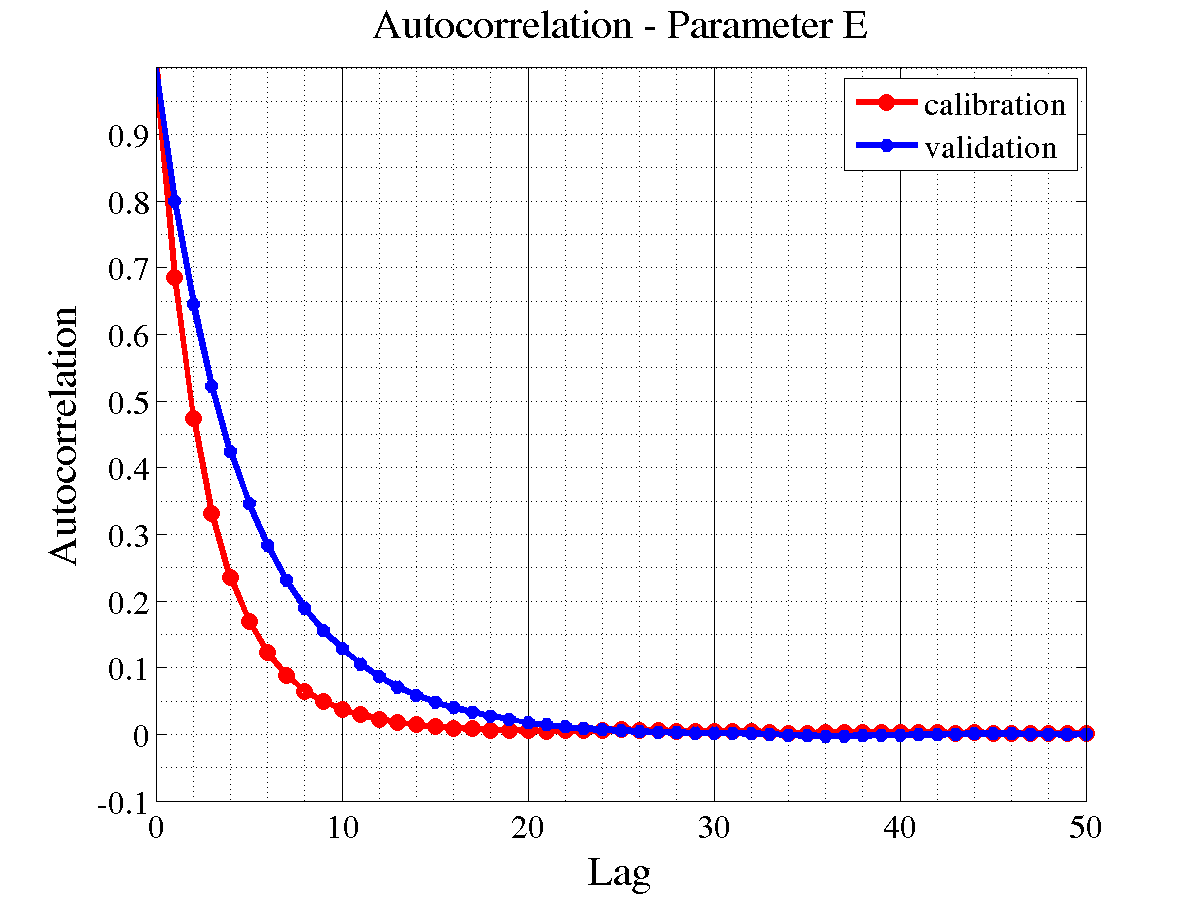
\includegraphics[scale=0.3]{figs/cal_val_parameter2_autocorrelation.png}}
\vspace*{-10pt}
\caption{Autocorrelation of parameters $A$ and $E$ (filtered chain).}
\label{fig:tga_ip_autocorrelation_param}
\end{figure}


\subsubsection{KDE, CDF and Autocorrelation Plots of QoI}
Figures \ref{fig:tga_pdf_qoi}  and \ref{fig:tga_cdf_qoi} present PDF and CDF of QoI, respectively and Figure \ref{fig:tga_autocorrelation_qoi} presents its autocorrelation.


\begin{figure}[p]
\centering 
\subfloat[QoI PDF]{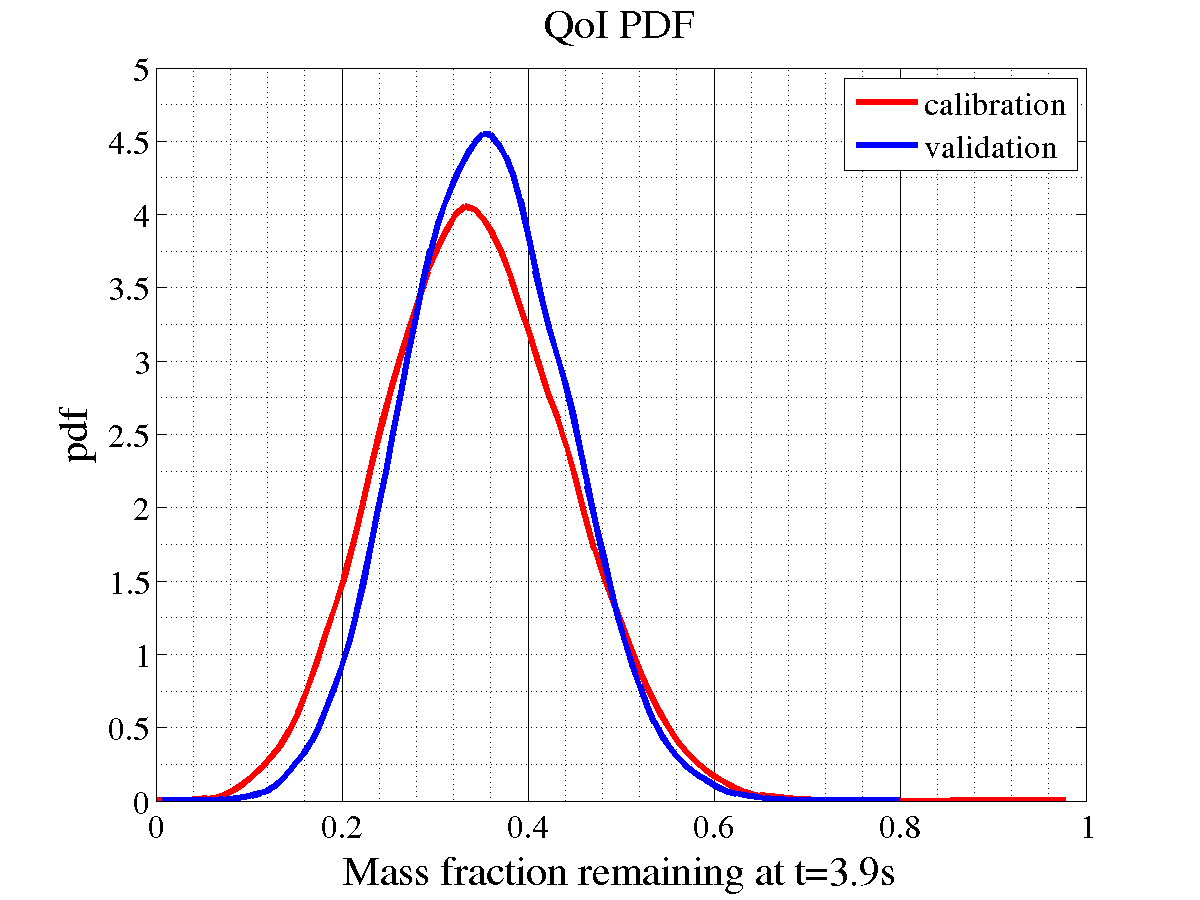
\includegraphics[scale=0.3]{figs/cal_val_QoI_PDF.png}\label{fig:tga_pdf_qoi}}
\subfloat[QoI CDF]{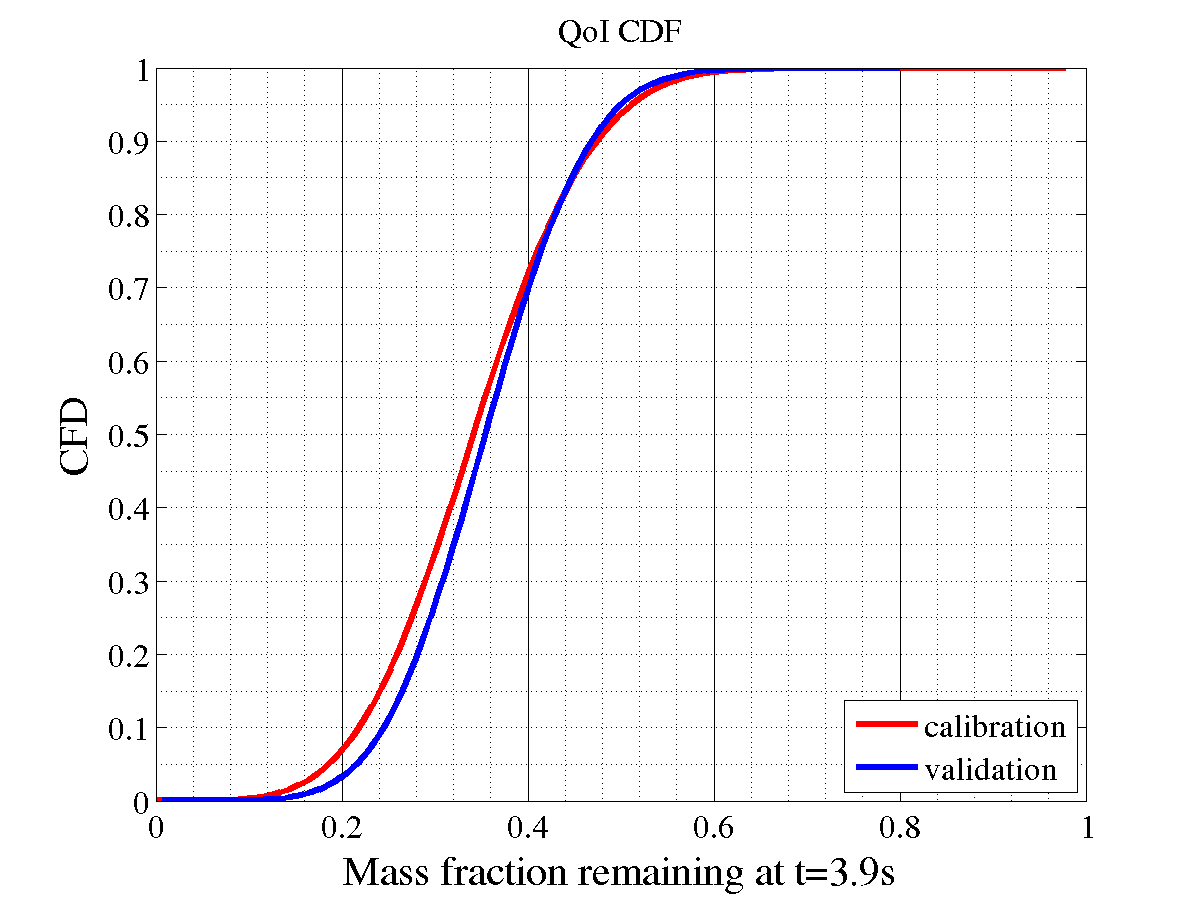
\includegraphics[scale=0.3]{figs/cal_val_QoI_CDF.png}\label{fig:tga_cdf_qoi}}
\vspace*{-10pt}
\caption{QoI PDF and CDF, during calibration and validation stages.}
\end{figure}


%
% \begin{figure}[htb]
% \centering
% 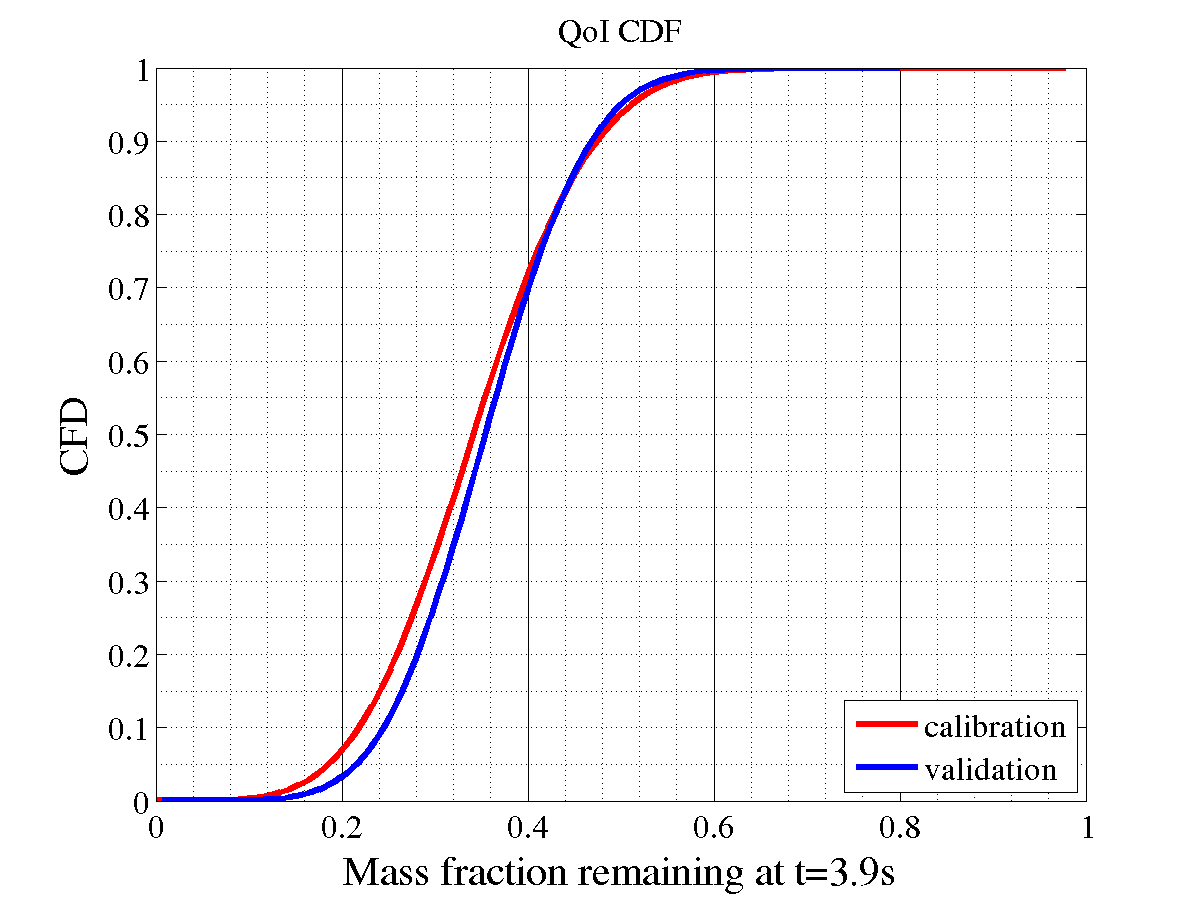
\includegraphics[scale=0.35]{figs/cal_val_QoI_CDF.png}
% \vspace*{-10pt}
% \caption{QoI CDF, during calibration and validation stages.}
% \label{fig:tga_cdf_qoi}
% \end{figure}

\begin{figure}[p]
\centering 
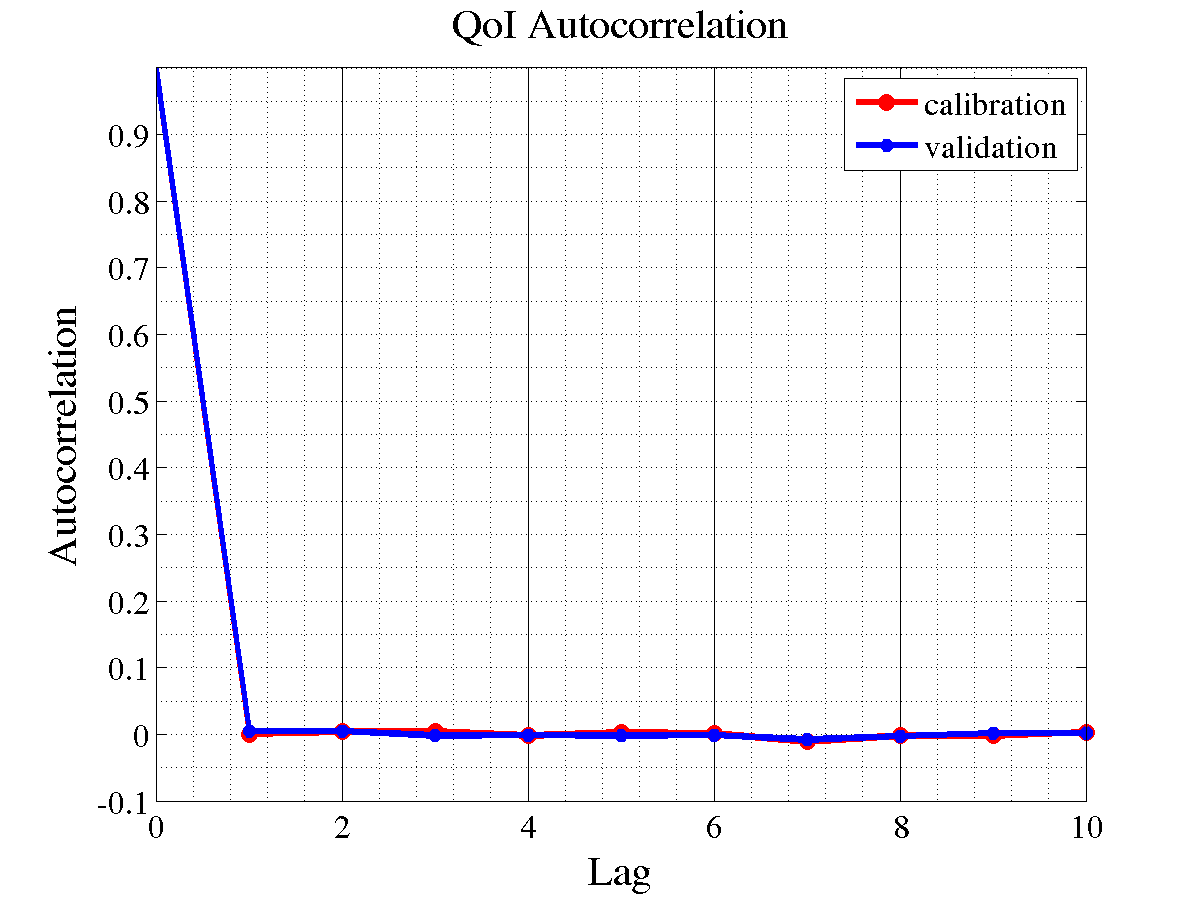
\includegraphics[scale=0.3]{figs/cal_val_QoI_autocorrelation}
\vspace*{-10pt}
\caption{QoI autocorrelation.}
\label{fig:tga_autocorrelation_qoi}
\end{figure}


\section{\texttt{modal}}\label{sec:example_modal}


This example presents a combination of two statistical inverse problems in one. 
It presents the capability of the Multilevel method in sampling from a target distribution that has either one or two modes (distinct peaks). The random variable of interest has three parameters, i.e., $\bv{\theta}=(\theta_1,\theta_2, \sigma^2) \in \mathbb{R}^3$, where the third parameter may be seen as variation.

The example also it gives the user the opportunity to chose either one single type of prior distribution, uniform, for the three components of the random variable, or two different priors: a uniform and a beta distribution.

Choosing between a one-mode or a two-mode target distribution is done at execution level, as presented in the following code line:

\begin{lstlisting}[label={},caption={}]
$ cd $HOME/LIBRARIES/QUESO-0.50.0/
$ cd examples/modal
$ rm outputData/*
$ ./modal_gsl example.inp <num_of_nodes>
\end{lstlisting}
where \verb+<num_of_nodes>+ is either 1 or 2.
% 
% 
% This simple statistical inverse problem presents a combination of two, suppose a random variable of interest with three parameters $\bv{\theta}=(\theta_1,\theta_2, \sigma) \in \mathbb{R}^3$,  namely $\bv{\theta}:[0,3]\times[0,3]\times[0,0.3] \rightarrow\mathbb{R}$. 
% 
% 
% 
% This simple statistical inverse problem, suppose a random variable of interest with three parameters $\bv{\theta}=(\theta_1,\theta_2, \sigma) \in \mathbb{R}^3$,  namely $\bv{\theta}:[0,3]\times[0,3]\times[0,0.3] \rightarrow\mathbb{R}$. 
% 
% 
% Suppose also that the distribution we aim to sample has either one or two modes.
% 
\subsection{One-mode distribution}

In this case, the target distribution is assumed to have only one mode.
Suppose also that the random variable $\bv{\theta}$  can either have a uniform prior distribution for all its components, i.e.:
$$
% \pi_{\text{prior}}=\mathcal{U}([0,3],[0,3],[0,0.3]).
\pi_{\text{prior}}=\mathcal{U}([0,3]) \times \mathcal{U}([0,3]) \times \mathcal{U}([0,0.3]).
$$
or, the prior distribution is defined as a combination of uniform prior for $\theta_1$ and $\theta_2$, with a beta prior for $\sigma^2$:
$$
% \pi_{\text{prior}}=\mathcal{U}([0,3],[0,3],[0,0.3]).
\pi_{\text{prior}}=\mathcal{U}([0,3]) \times \mathcal{U}([0,3]) \times \mathcal{B}(\alpha,\beta), \quad \text{with} \quad \alpha=3 \quad\text{and}\quad \beta=0.09709133373799.
$$

The likelihood function is defined as follows:
\begin{equation}
\begin{split} \small
%\pi_{\text{likelihood}}(\mathbf{d}|\boldsymbol{\theta}) = 
\quad f(\D|\bv{\theta})= -\dfrac{5}{2} \log\left(2 \pi \sigma^2\right)-\dfrac{1}{2\sigma^2} &\Bigg[
 \left(10 \sqrt{10 \theta_1+20 \theta_2+10 \sqrt{\theta_1^2+4 \theta_2^2}}-72.0470\right)^2 +\\
&+\left(10 \sqrt{10 \theta_1+20 \theta_2+10 \sqrt{\theta_1^2+4 \theta_2^2}}-71.8995\right)^2 +\\
&+\left(10 \sqrt{10 \theta_1+20 \theta_2+10 \sqrt{\theta_1^2+4 \theta_2^2}}-72.2801\right)^2 +\\
&+\left(10 \sqrt{10 \theta_1+20 \theta_2+10 \sqrt{\theta_1^2+4 \theta_2^2}}-71.9421\right)^2 +\\
&+\left(10 \sqrt{10 \theta_1+20 \theta_2+10 \sqrt{\theta_1^2+4 \theta_2^2}}-72.3578\right)^2 \Bigg].
\end{split}
\end{equation}

\subsubsection{Running the One-Mode Example}
 
To run the executable provided considering a \underline{one-mode} distribution, enter the following commands:
\begin{lstlisting}[label={},caption={Running the example with a one-mode distribution.}]
$ cd $HOME/LIBRARIES/QUESO-0.50.0/
$ cd examples/modal
$ rm outputData/*
$ ./modal_gsl example.inp 1      #one mode!
$ matlab
   $  plot_modal_all_levels_1mode  # inside matlab
   $ exit                          # inside matlab
$ ls -l outputData/*.png
modal_1_mode_kde_target.png  modal_1_mode_level_1.png  modal_1_mode_level_5.png
modal_1_mode_kde_theta1.png  modal_1_mode_level_2.png  modal_1_mode_level_6.png
modal_1_mode_kde_theta2.png  modal_1_mode_level_3.png  modal_1_mode_level_7.png
modal_1_mode_kde_theta3.png  modal_1_mode_level_4.png
\end{lstlisting}

As a result, the user should have created several of PNG figures scatter plots of each one of the levels and the kernel density estimation of the parameters, for each level in the Multilevel method. The name of the figure files have been chosen to be informative, as shown in the Listing above. 



\subsection{Two-mode distribution}

In this case, the target distribution is assumed to have two modes.
Suppose that $\bv{\theta}$ has a either uniform distribution for all its components, i.e.:
$$
% \pi_{\text{prior}}=\mathcal{U}([0,3],[0,3],[0,0.3]).
\pi_{\text{prior}}=\mathcal{U}([0,3]) \times \mathcal{U}([0,3]) \times \mathcal{U}([0,0.3]).
$$
or, the prior distribution is defined as a combination of uniform prior for the $\theta_1$, with a beta prior for $\theta_2$:
$$
% \pi_{\text{prior}}=\mathcal{U}([0,3],[0,3],[0,0.3]).
\pi_{\text{prior}}=\mathcal{U}([0,3]) \times \mathcal{U}([0,3]) \times \mathcal{B}(\alpha,\beta), \quad \text{with} \quad \alpha=3 \quad\text{and}\quad \beta=0.08335837191688.
$$

The likelihood function is defined as follows:
\begin{equation}
\begin{split}\small
f(\D|\bv{\theta})=  -5 \log\left(2 \pi \sigma^2\right)- \dfrac{1}{2\sigma^2} &\Bigg[ 
  \left(10 \sqrt{10 \theta_1+20 \theta_2+10 \sqrt{\theta_1^2+4 \theta_2^2}}-72.0470\right)^2+\\
&+\left(10 \sqrt{10 \theta_1+20 \theta_2+10 \sqrt{\theta_1^2+4 \theta_2^2}}-71.8995\right)^2+\\
&+\left(10 \sqrt{10 \theta_1+20 \theta_2+10 \sqrt{\theta_1^2+4 \theta_2^2}}-72.2801\right)^2+\\
&+\left(10 \sqrt{10 \theta_1+20 \theta_2+10 \sqrt{\theta_1^2+4 \theta_2^2}}-71.9421\right)^2+\\
&+\left(10 \sqrt{10 \theta_1+20 \theta_2+10 \sqrt{\theta_1^2+4 \theta_2^2}}-72.3578\right)^2+\\
&+\left(10 \sqrt{10 \theta_1+20 \theta_2-10 \sqrt{\theta_1^2+4 \theta_2^2}}-28.0292\right)^2+\\
&+\left(10 \sqrt{10 \theta_1+20 \theta_2-10 \sqrt{\theta_1^2+4 \theta_2^2}}-27.3726\right)^2+\\
&+\left(10 \sqrt{10 \theta_1+20 \theta_2-10 \sqrt{\theta_1^2+4 \theta_2^2}}-27.5388\right)^2+\\
&+\left(10 \sqrt{10 \theta_1+20 \theta_2-10 \sqrt{\theta_1^2+4 \theta_2^2}}-27.0357\right)^2+\\
&+\left(10 \sqrt{10 \theta_1+20 \theta_2-10 \sqrt{\theta_1^2+4 \theta_2^2}}-27.1588\right)^2 \Bigg].
\end{split} 
\end{equation}




\subsubsection{Running the Two-Mode Example}
 
To run the executable provided considering a \underline{two-modes} distribution, enter the following commands:
\begin{lstlisting}[label={},caption={Running the example with a two-mode distribution.}]
$ cd $HOME/LIBRARIES/QUESO-0.50.0/
$ cd examples/modal
$ rm outputData/*
$ ./modal_gsl example.inp 2         # two modes!
$ matlab
   $  plot_modal_all_levels_2modes  # inside matlab
   $ exit                           # inside matlab
$ ls -l outputData/*.png
modal_2_modes_kde_target.png  modal_2_modes_level_1.png  modal_2_modes_level_5.png
modal_2_modes_kde_theta1.png  modal_2_modes_level_2.png  modal_2_modes_level_6.png
modal_2_modes_kde_theta2.png  modal_2_modes_level_3.png  modal_2_modes_level_7.png
modal_2_modes_kde_theta3.png  modal_2_modes_level_4.png  modal_2_modes_level_8.png
\end{lstlisting}

As a result, the user should have created several of PNG figures scatter plots of each one of the levels and the kernel density estimation of the parameters, for each level in the Multilevel method. The name of the figure files have been chosen to be informative, as shown in the Listing above. 



\subsection{Example Code}\label{sec:modal-code}

The source code for the example is composed of 5 files:
\texttt{example\_main.C} (Listing \ref{code:modal-main-c}), \linebreak
\texttt{example\_likelihood.h} and \texttt{example\_likelihood.C} (Listings \ref{fig-like-modal-h} and \ref{fig-like-modal-c}),
\texttt{example\_compute.h} and \texttt{example\_compute.C} (Listings \ref{code:modal-compute-h} and \ref{code:modal-compute-c}).


\lstinputlisting[caption=File \texttt{example\_main.C.}, label={code:modal-main-c}, linerange={33-1000}]{../../examples/modal/src/example_main.C}

\lstinputlisting[caption=File \texttt{example\_likelihood.h}., label={fig-like-modal-h}, linerange={32-1000}]{../../examples/modal/src/example_likelihood.h}

\lstinputlisting[caption=File \texttt{example\_likelihood.C}., label={fig-like-modal-c}, linerange={33-1000}]{../../examples/modal/src/example_likelihood.C}

\lstinputlisting[caption=File \texttt{example\_compute.h.}, label={code:modal-compute-h}, linerange={32-1000}]{../../examples/modal/src/example_compute.h}


Note that in line 12 of Listings \ref{code:modal-compute-c} the \verb+#define+ directive creates the macro
 \linebreak
\verb+APPLS_MODAL_USES_CONCATENATION+. Such macro, together with the directives \verb+#ifdef+, \verb+#else+, and \verb+#endif+, tells the compiler that the application will use concatenated priors, by controlling compilation of portions of file \texttt{example\_compute.C}. Commenting line 12 of Listings \ref{code:modal-compute-c} will make the application to use uniform priors only:

\lstinputlisting[caption={File \texttt{example\_compute.C}.}, label={code:modal-compute-c}, linerange={33-1000},numbers=left]{../../examples/modal/src/example_compute.C}
 
  


\subsection{Input File}\label{sec:modal-input-file}


QUESO reads an input file for solving statistical problems, which provides options for the Multilevel or MCMC method. In this example, the Multilevel method is chosen to sample from the distribution. Many variables are common to both MCMC and Multilevel method, especially because the Multilevel method also has the option of delaying the rejection of a candidate. The names of the variables have been designed to be informative in this case as well:
\begin{description}\vspace{-8pt}
\item[ \texttt{env}:] refers to QUESO environment; \vspace{-8pt}
\item[ \texttt{ip}:] refers to inverse problem;\vspace{-8pt}
\item[ \texttt{ml}:] refers to Multilevel;\vspace{-8pt}
\item[ \texttt{dr}:] refers to delayed rejection;\vspace{-8pt}
\item[ \texttt{rawChain}:] refers to the raw, entire chain; \vspace{-8pt}
\item[ \texttt{filteredChain}:] refers to a filtered chain (related to a specified \texttt{lag});\vspace{-8pt}
\item[ \texttt{last}:] refers to instructions specific for the last level of the Multilevel algorithm.
\end{description}

The user may select options for a specific level by naming its number, i.e., in case the user wants to write the raw chain of the level 3 in a separate file, say \verb+'rawChain_ml_level3.m'+, he/she may include the line: 
\begin{lstlisting}
ip_ml_3_rawChain_dataOutputFileName = outputData/rawChain_ml_level3 
\end{lstlisting}
in the input file.


The options used for solving this example are displayed in Listing \ref{code:modal-input-file}. 

\lstinputlisting[caption={Options for QUESO library used in application code (Listings \ref{code:modal-main-c}-\ref{code:modal-compute-c}})., 
label={code:modal-input-file},]{../../examples/modal/tests/test_2013_11_22/example.inp}



\subsection{Create your own Makefile}\label{sec:modal-makefile}

Makefiles are special format files that together with the make utility will help one to compile and automatically build and manage projects (programs).  
Listing \ref{code:modal_makefile} presents a Makefile, named `\texttt{Makefile\_modal\_example\_margarida}', that may be used to compile the code and create the executable \verb+modal_gsl+. Naturally, it must be adapted to the user's settings, i.e., it has to have the correct paths for the user's libraries that have actually been used to compile and install QUESO  (see Sections \ref{sec:Pre_Queso}--\ref{sec:install_Queso_make}).

\lstinputlisting[caption={Makefile for the application code in Listings \ref{code:modal-main-c}-\ref{code:modal-compute-c}},  label={code:modal_makefile},language={bash}]{../../examples/modal/src//Makefile_modal_violeta}

Thus, to compile, build and execute the code, the user just needs to run the following commands in the same directory where the files are:
\begin{lstlisting}
$ cd $HOME/LIBRARIES/QUESO-0.50.0/examples/modal/
$ export LD_LIBRARY_PATH=$LD_LIBRARY_PATH:\
  $HOME/LIBRARIES/gsl-1.15/lib/:\
  $HOME/LIBRARIES/boost-1.53.0/lib/:\
  $HOME/LIBRARIES/hdf5-1.8.10/lib:\
  $HOME/LIBRARIES/QUESO-0.50.0/lib 
$ make -f Makefile_modal_violeta 
$ ./modal_gsl example.inp <num_modes>
\end{lstlisting}

The `\verb+export+' instruction above is only necessary if the user has not saved it in his/her \verb+.bashrc+ file. 


\subsection{Data Post-Processing and Visualization}\label{sec:modal-results}



According to the specifications of the input file in Listing~\ref{code:modal-input-file}, both a folder named \verb+outputData+ and a the following files should be generated:
\begin{verbatim}
rawChain_ml.m 
display_sub0.txt    
\end{verbatim}


The sequence of Matlab commands is identical to the ones presented in Sections
\ref{sec:sip-results}, \ref{sec:sfp-results}, \ref{sec:gravity-results} and \ref{sec:tga-results};
therefore, are omitted here. The reader is invited to explore the Matlab files
\texttt{plot\_modal\_all\_levels\_1mode.m}  and/or \texttt{plot\_modal\_all\_levels\_2modes.m}  
%\texttt{validationCycle/tests/test\_2012\_11\_15/tga\_cycle\_plot.m} 
for details of how the figures have been generated.


\subsubsection{Scatter Plots}

The code presented in Listing \ref{matlab:modal_scatter} uses Matlab function \verb+plotmatrix+ to generate Figures \ref{fig:modal_scatter_1mode} and \ref{fig:modal_scatter_2modes}
which presents the scatter plots and histograms of the parameters $\theta_1$ and $\theta_2$, based on the generated raw chains. 


\begin{lstlisting}[label=matlab:modal_scatter,caption={Matlab code for the scatter plots depicted in Figures \ref{fig:modal_scatter_1mode} and \ref{fig:modal_scatter_2modes}.}]
fprintf(1,'Scatter plots and histograms of raw chains - Level 1 <press any key>\n');
plotmatrix(ip_ml_1_rawChain_unified, '+b')
set(gca,'fontsize',20); 
xlabel('\theta_1                  \theta_2                   \theta_3','fontsize',16);
ylabel('\theta_3                  \theta_2                   \theta_1','fontsize',16);
title('Scatter plots and histograms, Level 1 - 1 mode')
\end{lstlisting}

\begin{figure}[htpb]
\centering
%\subfloat[$\theta_1$]{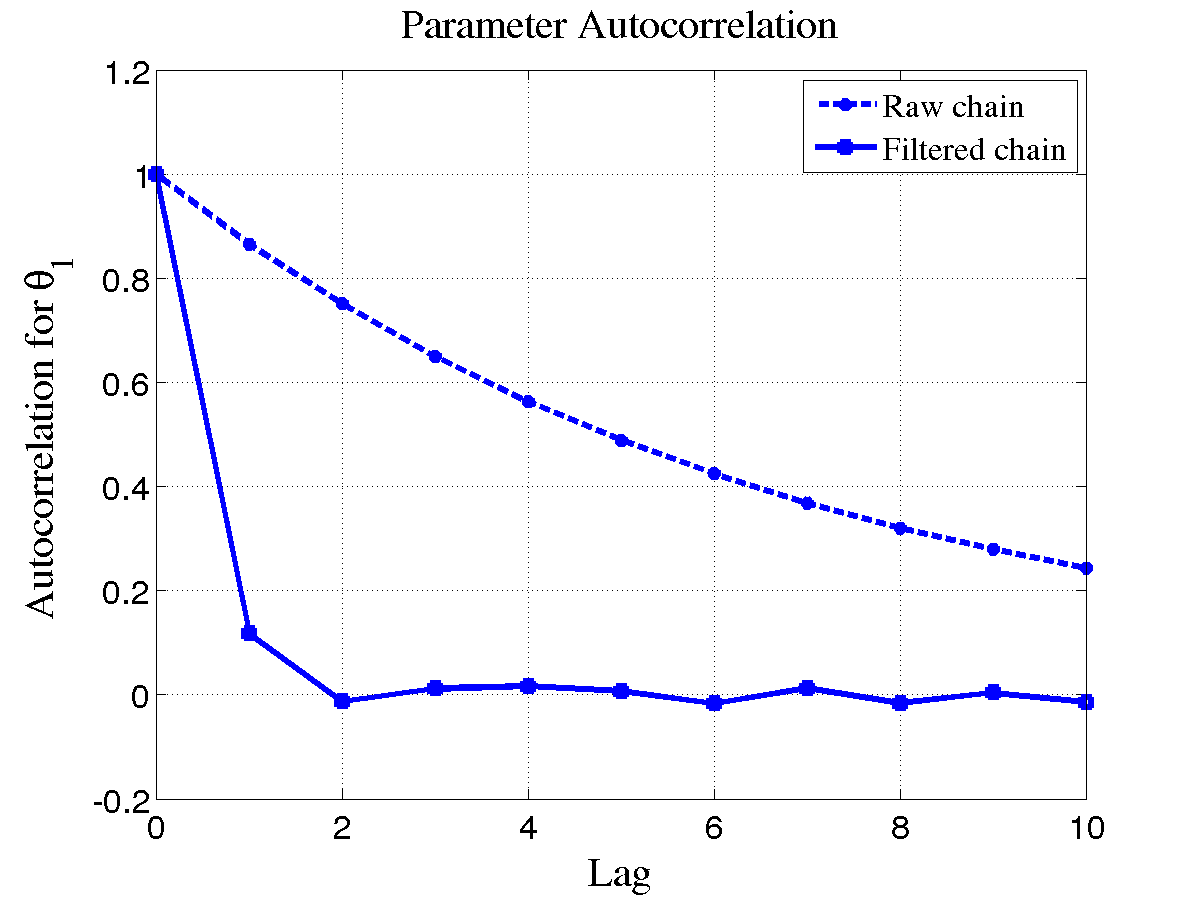
\includegraphics[scale=0.35]{figs/simple_ip_autocorrelation_raw_filt_theta1.png}}
%\subfloat[$\theta_2$]{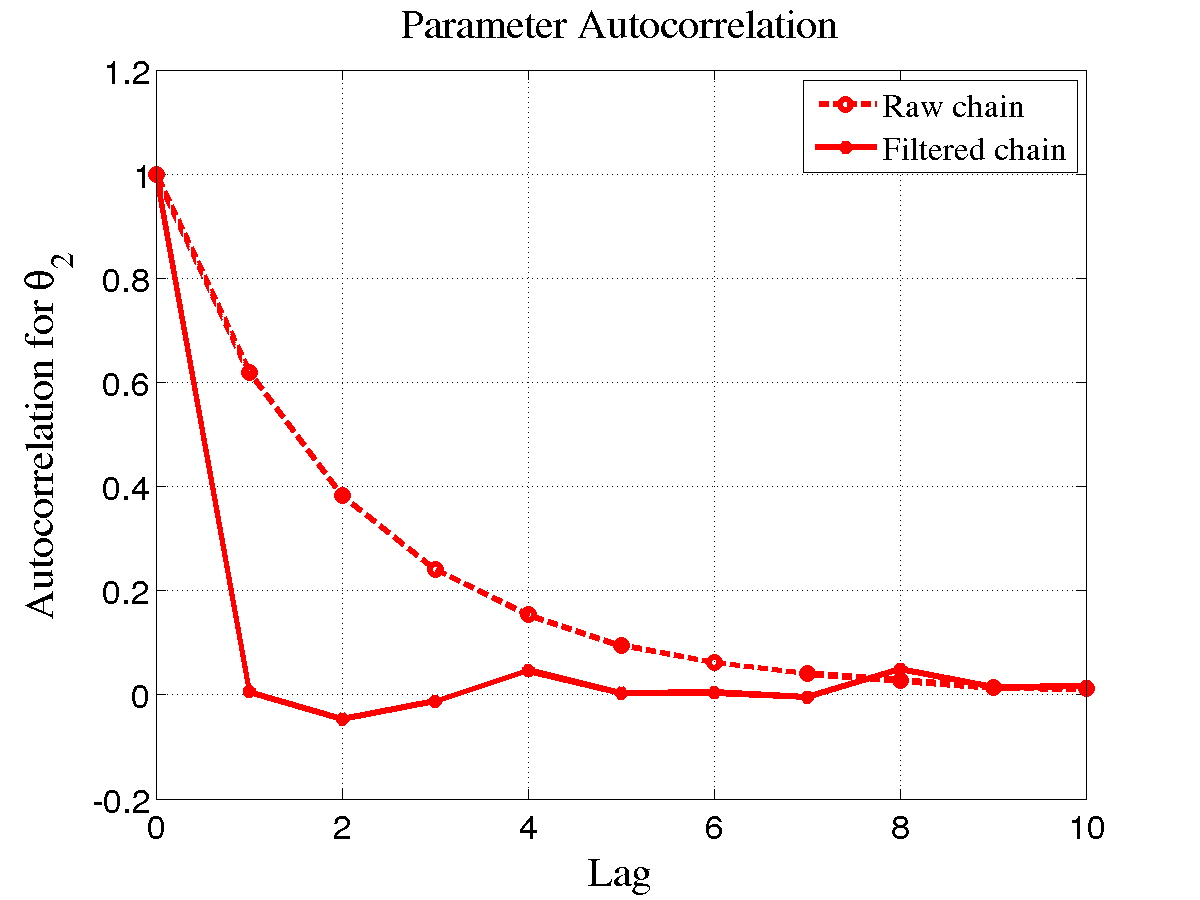
\includegraphics[scale=0.35]{figs/simple_ip_autocorrelation_raw_filt_theta2.png}}
\subfloat{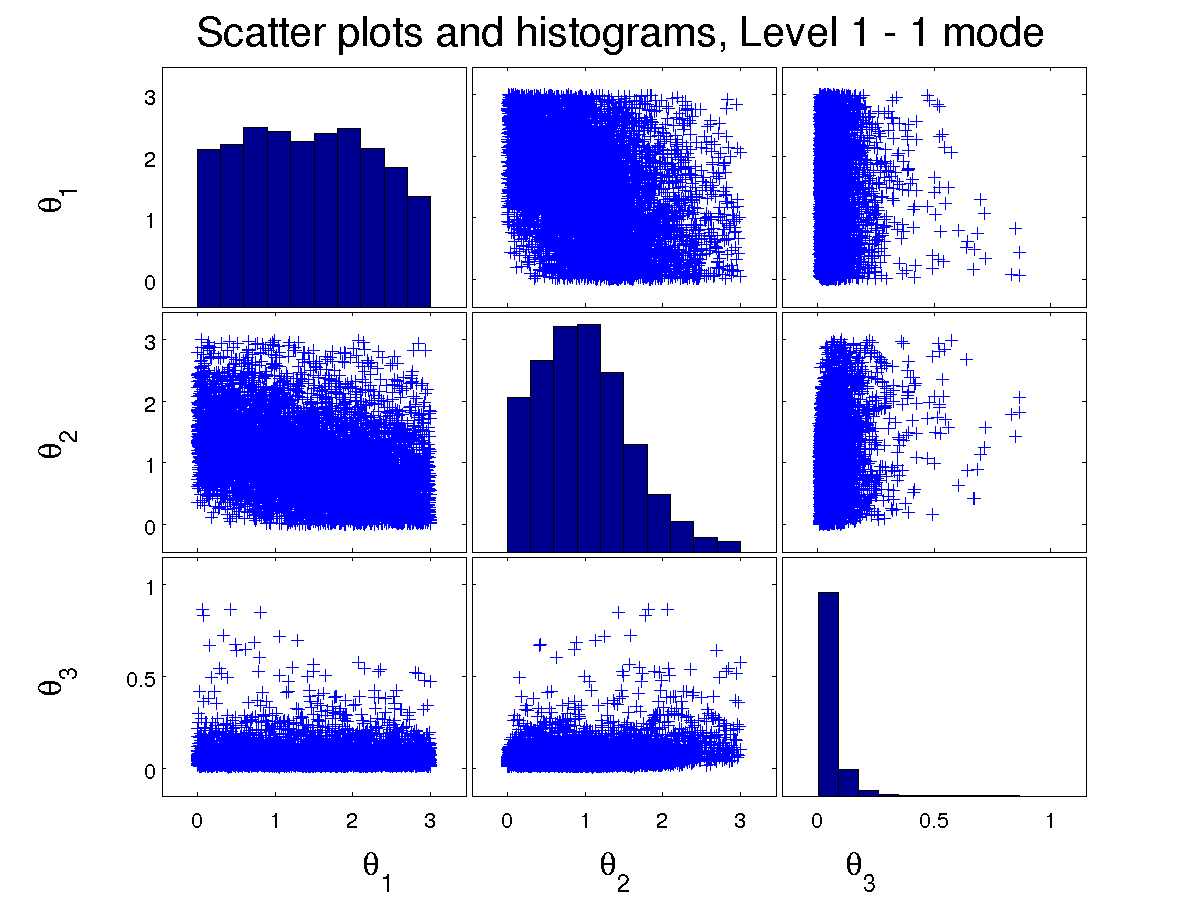
\includegraphics[scale=0.3]{figs/modal_1_mode_level_1.png}}
\subfloat{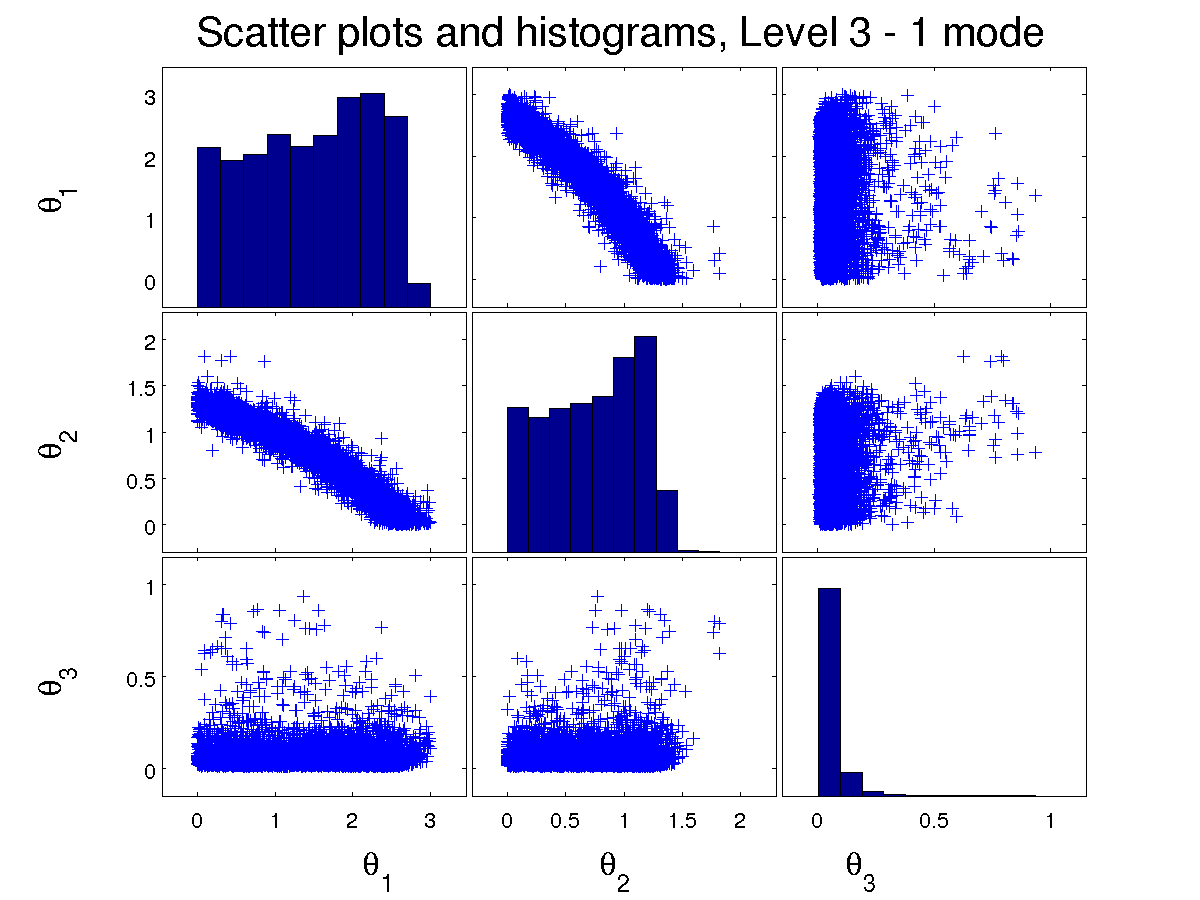
\includegraphics[scale=0.3]{figs/modal_1_mode_level_3.png}}\\
\subfloat{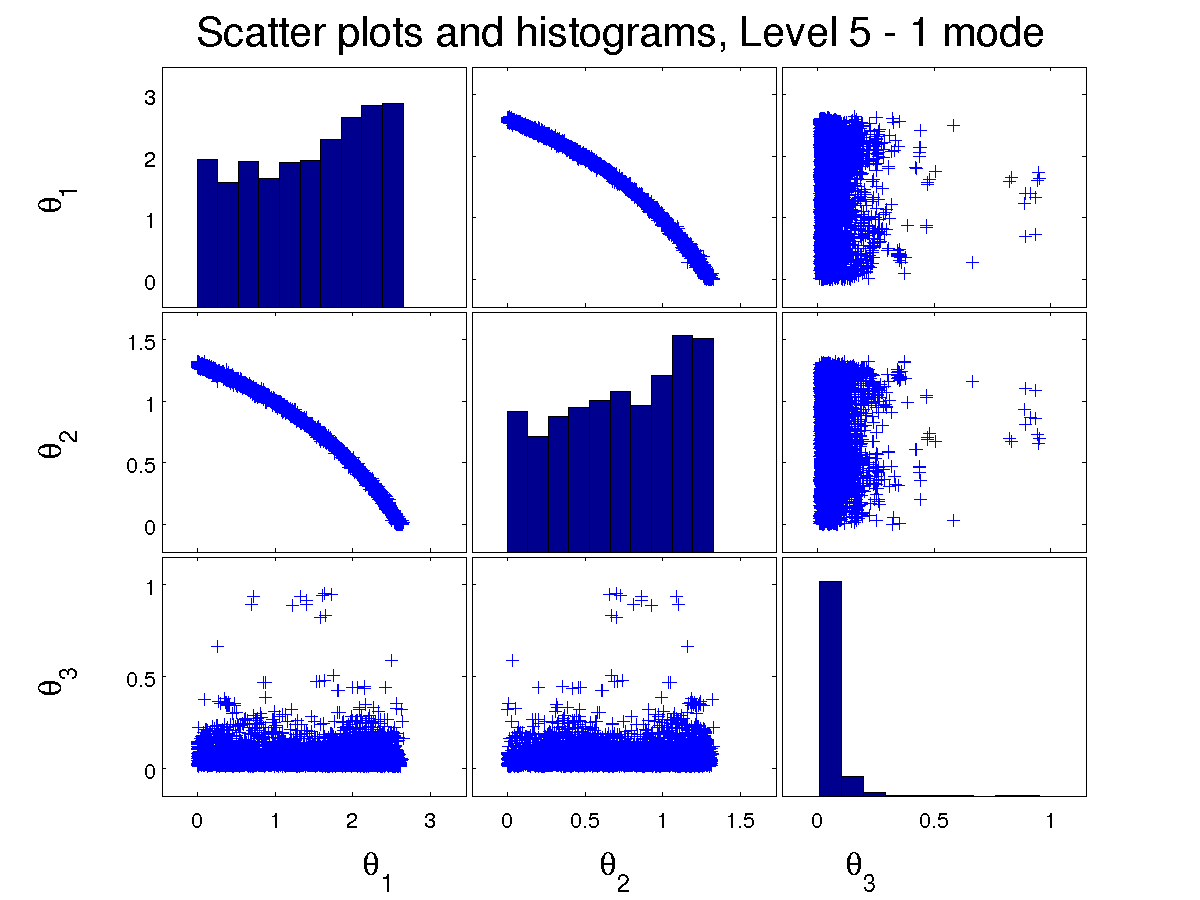
\includegraphics[scale=0.3]{figs/modal_1_mode_level_5.png}}
\subfloat{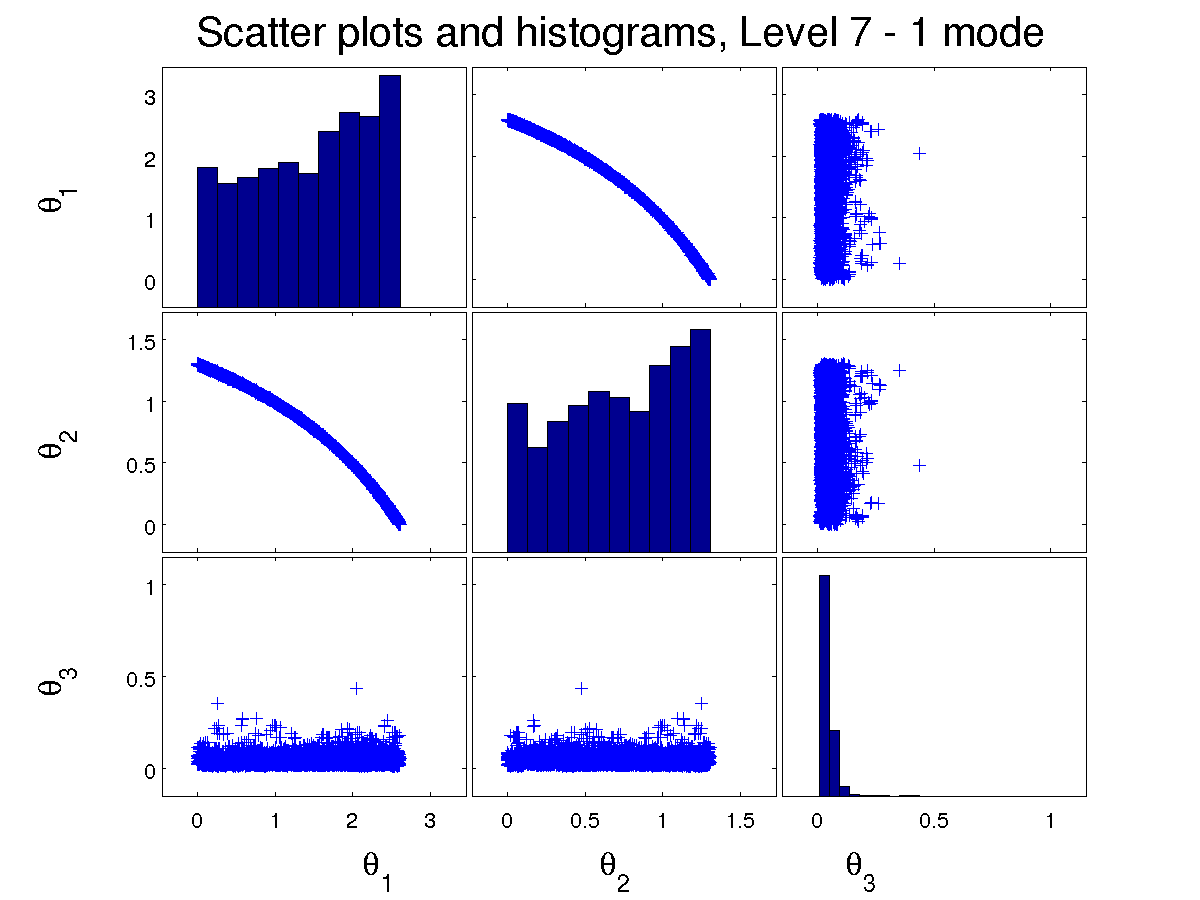
\includegraphics[scale=0.3]{figs/modal_1_mode_level_7.png}}
\vspace{-10pt}
\caption{Scatter plots for $\theta_1$, $\theta_2$ and $\theta_3=\sigma^2$, levels 1, 3, 5 and 7 (last). One mode distribution.}
\label{fig:modal_scatter_1mode}
\end{figure}

\begin{figure}[htpb]
\centering
%\subfloat[$\theta_1$]{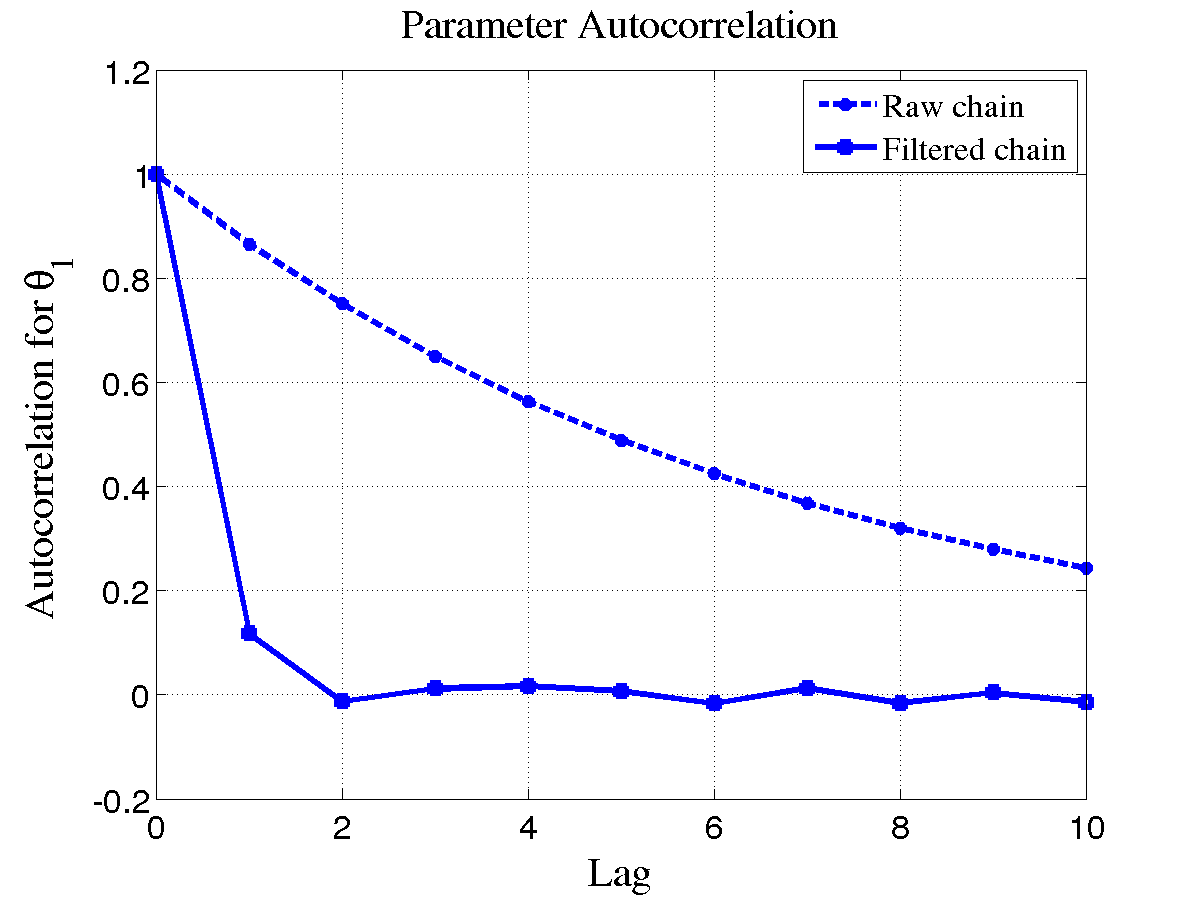
\includegraphics[scale=0.35]{figs/simple_ip_autocorrelation_raw_filt_theta1.png}}
%\subfloat[$\theta_2$]{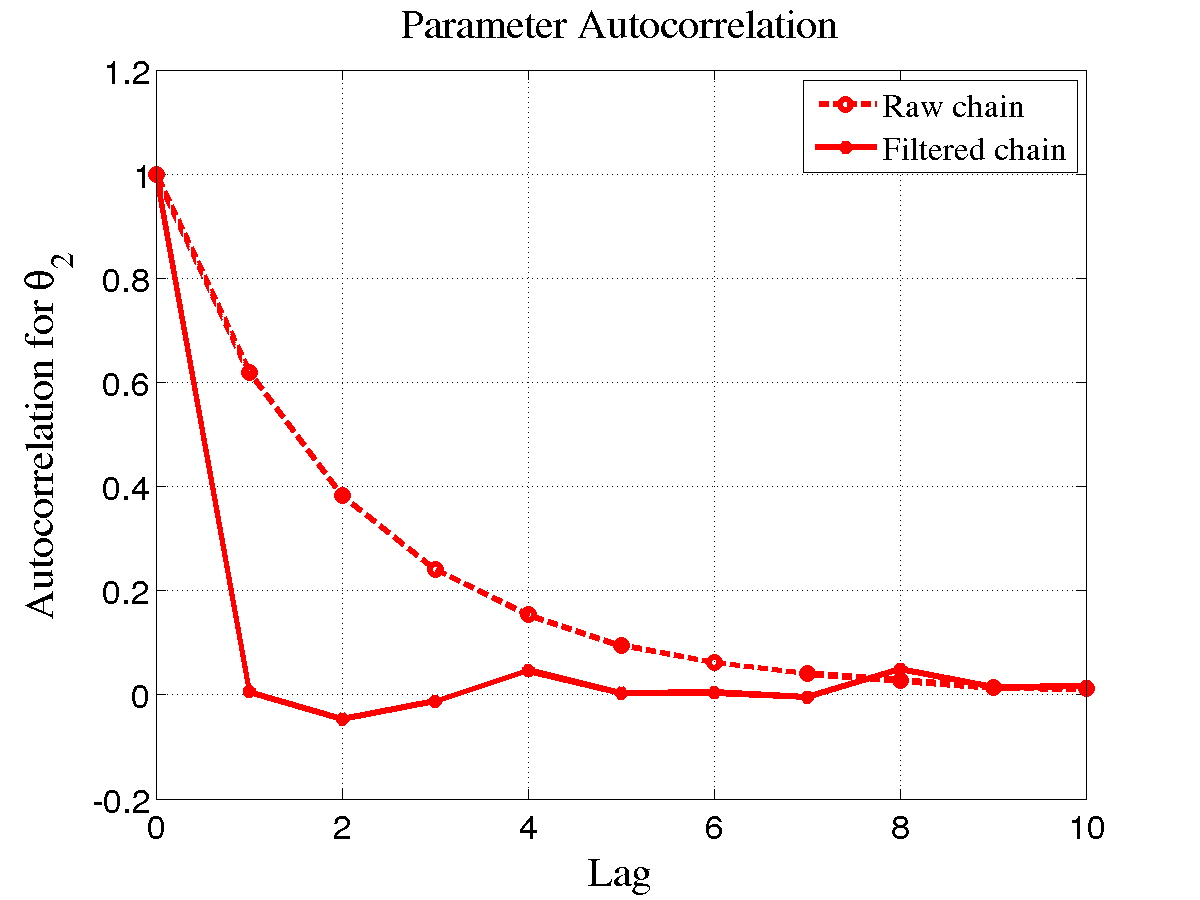
\includegraphics[scale=0.35]{figs/simple_ip_autocorrelation_raw_filt_theta2.png}}
\subfloat{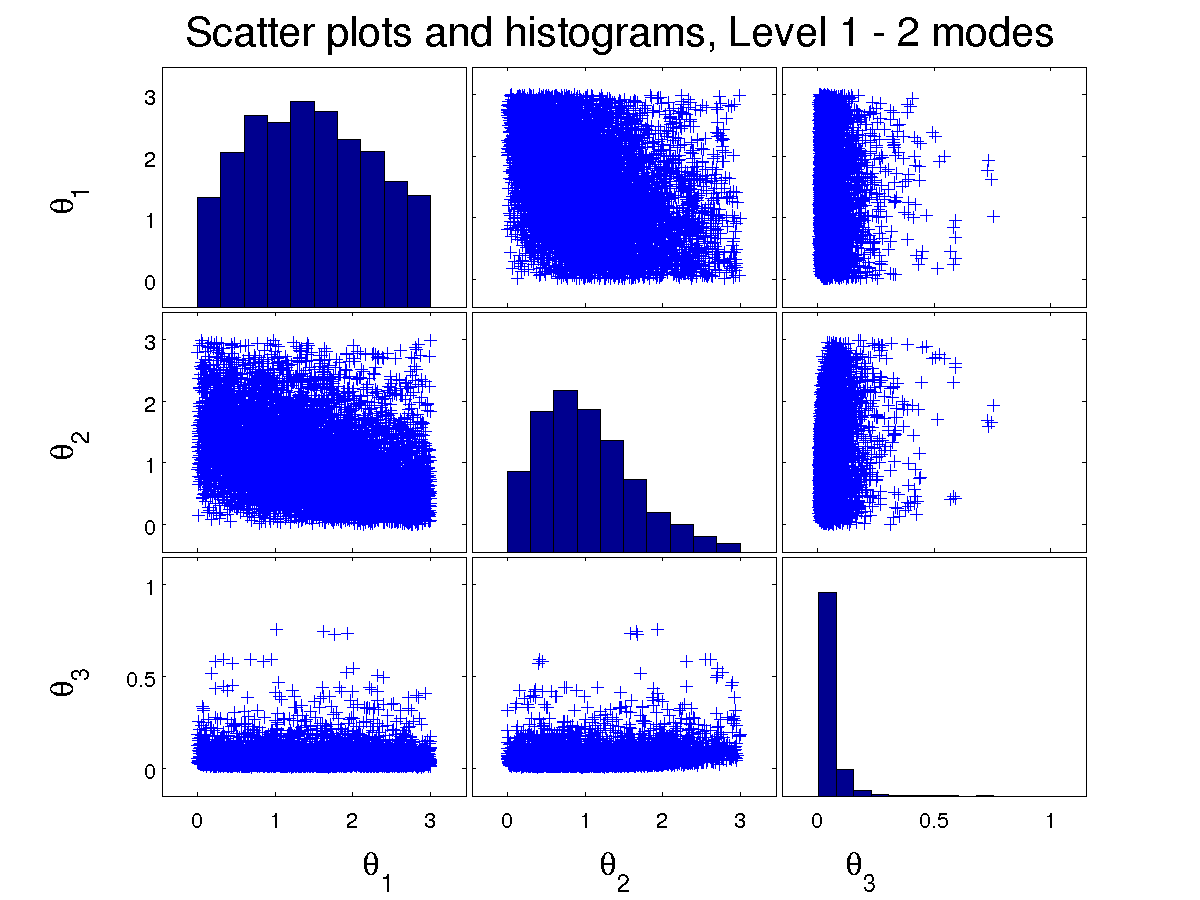
\includegraphics[scale=0.3]{figs/modal_2_modes_level_1.png}}
\subfloat{\includegraphics[scale=0.3]{figs/modal_2_modes_level_3.png}}\\
\subfloat{\includegraphics[scale=0.3]{figs/modal_2_modes_level_6.png}}
\subfloat{\includegraphics[scale=0.3]{figs/modal_2_modes_level_9.png}}
\vspace{-10pt}
\caption{Scatter plots for $\theta_1$, $\theta_2$ and $\theta_3=\sigma^2$, levels 1, 3, 6 and 9 (last). Two-mode distribution.}
\label{fig:modal_scatter_2modes}
\end{figure}

\subsubsection{KDE Plots}

Figures \ref{fig:modal_kde_1mode} and \ref{fig:modal_kde_2modes} present the KDE plots of the parameters $\theta_1$, $\theta_2$, $\theta_3$ and target PDF in both cases: one-mode and two-modes distribution. 



\begin{figure}[hptb]
\centering
\subfloat{\includegraphics[scale=0.3]{figs/modal_1_mode_kde_theta1.png}}
\subfloat{\includegraphics[scale=0.3]{figs/modal_1_mode_kde_theta2.png}}\\
\subfloat{\includegraphics[scale=0.3]{figs/modal_1_mode_kde_theta3.png}}
\subfloat{\includegraphics[scale=0.3]{figs/modal_1_mode_kde_target.png}}
\vspace{-10pt}
\caption{KDE plots for $\theta_1$, $\theta_2$, $\theta_3=\sigma^2$, and the target PDF. One mode distribution.}
\label{fig:modal_kde_1mode}
\end{figure}

\begin{figure}[hptb]
\centering
\subfloat{\includegraphics[scale=0.3]{figs/modal_2_modes_kde_theta1.png}}
\subfloat{\includegraphics[scale=0.3]{figs/modal_2_modes_kde_theta2.png}}\\
\subfloat{\includegraphics[scale=0.3]{figs/modal_2_modes_kde_theta3.png}}
\subfloat{\includegraphics[scale=0.3]{figs/modal_2_modes_kde_target.png}}
\vspace{-10pt}
\caption{KDE plots for $\theta_1$, $\theta_2$, $\theta_3=\sigma^2$, and the target PDF. Two-mode distribution.}
\label{fig:modal_kde_2modes}
\end{figure}


\subsubsection{Autocorrelation Plots}

Figures \ref{fig:modal_autocorr_1mode} and \ref{fig:modal_autocorr_2modes} present the autocorrelation of the parameters $\theta_1$, $\theta_2$ and $\theta_3$ in both cases: one-mode and two-modes distribution.

\begin{figure}[htpb]
\centering
\subfloat{\includegraphics[scale=0.25]{figs/modal_1_mode_autocorrelation_theta1.png}}
\subfloat{\includegraphics[scale=0.25]{figs/modal_1_mode_autocorrelation_theta2.png}}
\subfloat{\includegraphics[scale=0.25]{figs/modal_1_mode_autocorrelation_theta3.png}}
\vspace{-10pt}
\caption{Autocorrelation plots for $\theta_1$, $\theta_2$ and $\theta_3=\sigma^2$. One-mode distribution.}
\label{fig:modal_autocorr_1mode}
\end{figure}

\begin{figure}[htpb]
\centering
\subfloat{\includegraphics[scale=0.25]{figs/modal_2_modes_autocorrelation_theta1.png}}
\subfloat{\includegraphics[scale=0.25]{figs/modal_2_modes_autocorrelation_theta2.png}}
\subfloat{\includegraphics[scale=0.25]{figs/modal_2_modes_autocorrelation_theta3.png}}
\vspace{-10pt}
\caption{Autocorrelation plots for $\theta_1$, $\theta_2$ and $\theta_3=\sigma^2$. Two-mode distribution.}
\label{fig:modal_autocorr_2modes}
\end{figure}

\section{\texttt{bimodal}}\label{sec:example_bimodal}


This example replicates the problem in ``Section 4.1 A 1D Problem'' of~\cite{CheungPrudencio2012}: it presents how to use QUESO and the Multilevel method for sampling from a posterior PDF composed of the sum of two Gaussian distributions. 

Let's define $D=[-250,250]$ and the three distributions $\pi_\prior: D \rightarrow \mathbb{R}_+ $, $f_1: \mathbb{R} \rightarrow \mathbb{R}_+ $ and $f_2: \mathbb{R} \rightarrow \mathbb{R}_+$ by:
\begin{equation}
\begin{split}\label{eq:bimodal_functions}
\pi_\prior &=  \dfrac{1}{|D|} = \dfrac{1}{500}, \quad \forall \,  \theta \in D \\
f_1(\theta) &= \dfrac{1}{(2\pi)^{1/2} \sqrt{|V_1|}} \exp \left(-\dfrac{1}{2}(\theta - \mu_1)^T \, V_1^{-1} \, (\theta - \mu_1) \right), \quad \forall \,  \theta \in \mathbb{R} \\
f_2(\theta) &= \dfrac{1}{(2\pi)^{1/2} \sqrt{|V_2|}} \exp \left(-\dfrac{1}{2}(\theta - \mu_2)^T \, V_2^{-1} \, (\theta - \mu_2) \right), \quad \forall \, \theta \in \mathbb{R},
\end{split}
\end{equation}
where
\begin{equation*}
\mu_1 = 10, \quad  V_1 = 1^2, \quad \mu_2 = 100, \quad V_2= 5^2.
\end{equation*}

In this example, we want to sample the posterior PDF given by:
\begin{equation}
\pi_\post(\theta)  \propto \left[\dfrac{1}{2} f_1(\theta) + \dfrac{1}{2} f_2(\theta) \right] \cdot \pi_\prior = f(\theta) \cdot \pi_\prior
\end{equation}
where $f(\theta)= \dfrac{1}{2} f_1(\theta) + \dfrac{1}{2} f_2(\theta)$ is the likelihood function, which is depicted in Figure \ref{fig:bimodal:likelihood}.

\begin{figure}[htpb]
\centering
\includegraphics[scale=0.35]{figs/bimodal_likelihood.png}
\vspace{-10pt}
\caption{Likelihood function given by $f=f_1/2+ f_2/2$, where $f_1$ and $f_2$ are defined in Equation \eqref{eq:bimodal_functions}.}
\label{fig:bimodal:likelihood}
\end{figure}


\subsection{Running the Example}\label{sec:bimodal-run}

To run the executable provided (available after QUESO installation), and generate figures for the chains, PDFs, CDFs, etc., enter the following commands:
\begin{lstlisting}[label={},caption={}]
$ cd $HOME/LIBRARIES/QUESO-0.51.0/examples/bimodal
$ rm outputData/*
$ ./bimodal_gsl bimodal_1chain.inp    
$ matlab
   $ plot_all.m	                          # inside matlab
   $ plot_likelihood_normalized_taus.m    # inside matlab
   $ plot_likelihood_unnormalized_taus.m  # inside matlab
   $ exit                                 # inside matlab
$ ls -l outputData/*.png
bimodal_autocorrelation_rawchain.png  bimodal_likelihood.png
bimodal_cdf_rawchain.png	          bimodal_likelihood_taus_normalized.png
bimodal_kde_rawchain.png	          bimodal_likelihood_taus.png
\end{lstlisting}


As a result, the user should have created several of PNG figures containing marginal posterior PDF, cumulative density distribution and autocorrelation. The name of the figure files have been chosen to be informative, as shown in the Listing above.




\subsection{Example Code}\label{sec:bimodal-code}

The source code for the example is composed of 5 files:
\texttt{bimodal\_main.C} (Listing \ref{code:bimodal-main-c}), \linebreak
\texttt{bimodal\_likelihood.h} and \texttt{bimodal\_likelihood.C} (Listings \ref{fig-like-bimodal-h} and \ref{fig-like-bimodal-c}),
\texttt{bimodal\_compute.h} and \texttt{bimodal\_compute.C} (Listings \ref{code:bimodal-compute-h} and \ref{code:bimodal-compute-c}).


\lstinputlisting[caption=File \texttt{bimodal\_main.C.}, label={code:bimodal-main-c}, linerange={25-1000}]{../../examples/bimodal/src/bimodal_main.C}

\lstinputlisting[caption=File \texttt{bimodal\_likelihood.h}., label={fig-like-bimodal-h}, linerange={25-1000}]{../../examples/bimodal/src/bimodal_likelihood.h}

\lstinputlisting[caption=File \texttt{bimodal\_likelihood.C}., label={fig-like-bimodal-c}, linerange={25-1000}]{../../examples/bimodal/src/bimodal_likelihood.C}

\lstinputlisting[caption=File \texttt{bimodal\_compute.h.}, label={code:bimodal-compute-h}, linerange={25-1000}]{../../examples/bimodal/src/bimodal_compute.h}

Note that in line 57 of Listings \ref{code:bimodal-compute-c} the `\verb+#if 0+' directive tells the compiler that the application will not use DRAM algorithm, but rather the Multilevel solver (line 65). Naturally, the user may chose to use the DRAM algorithm by changing the directive in line 57 to `\verb+#if 1+'.

\lstinputlisting[caption={File \texttt{bimodal\_compute.C}.}, label={code:bimodal-compute-c}, linerange={25-1000},numbers=left]{../../examples/bimodal/src/bimodal_compute.C}
 
  


\subsection{Input File}\label{sec:bimodal-input-file}


QUESO reads an input file for solving statistical problems, which provides options for the Multilevel or MCMC method. In this example, the Multilevel method is chosen to sample from the distribution. Many variables are common to both MCMC and Multilevel method, especially because the Multilevel method also has the option of delaying the rejection of a candidate. The names of the variables have been designed to be informative in this case as well:
\begin{description}\vspace{-8pt}
\item[ \texttt{env}:] refers to QUESO environment; \vspace{-8pt}
\item[ \texttt{ip}:] refers to inverse problem;\vspace{-8pt}
\item[ \texttt{ml}:] refers to Multilevel;\vspace{-8pt}
\item[ \texttt{dr}:] refers to delayed rejection;\vspace{-8pt}
\item[ \texttt{rawChain}:] refers to the raw, entire chain; \vspace{-8pt}
\item[ \texttt{filteredChain}:] refers to a filtered chain (related to a specified \texttt{lag});\vspace{-8pt}
\item[ \texttt{last}:] refers to instructions specific for the last level of the Multilevel algorithm.
\end{description}

The user may select options for a specific level by naming its number, i.e., in case the user wants to define a different number of extra stages together with the scales for each stage (in the DRAM part of the ML algorithm) for the level 3, he/she may include the following instructions:
\begin{lstlisting}
ip_ml_3_dr_maxNumExtraStages          = 1
ip_ml_3_dr_listOfScalesForExtraStages = 3.333
\end{lstlisting}
in the input file.


The options used for solving this example are displayed in Listing \ref{code:bimodal-input-file}. 

\lstinputlisting[caption={Options for QUESO library used in application code (Listings \ref{code:bimodal-main-c}-\ref{code:bimodal-compute-c}})., 
label={code:bimodal-input-file},]{../../examples/bimodal/tests/test_2013_12_02/bimodal_1chain.inp}



\subsection{Create your own Makefile}\label{sec:bimodal-makefile}

Similarly to the other examples presented in this user's manual and also available with QUESO distribution, a user-created makefile is available: `\texttt{Makefile\_bimodal\_violeta}'. When adapted to the user's settings, namely paths for  QUESO required libraries, it may be used to compile the code and create the executable \verb+bimodal_gsl+. 

Thus, to compile, build and execute the code, the user just needs to run the following commands in the same directory where the files are:
\begin{lstlisting}
$ cd $HOME/LIBRARIES/QUESO-0.51.0/examples/bimodal/
$ export LD_LIBRARY_PATH=$LD_LIBRARY_PATH:\
  $HOME/LIBRARIES/gsl-1.15/lib/:\
  $HOME/LIBRARIES/boost-1.53.0/lib/:\
  $HOME/LIBRARIES/hdf5-1.8.10/lib:\
  $HOME/LIBRARIES/QUESO-0.51.0/lib 
$ make -f Makefile_bimodal_violeta 
$ ./bimodal_gsl example.inp
\end{lstlisting}

Again, the `\verb+export+' instruction above is only necessary if the user has not saved it in his/her \verb+.bashrc+ file. 


\subsection{Data Post-Processing and Visualization}\label{sec:bimodal-results}



According to the specifications of the input file in Listing~\ref{code:bimodal-input-file}, both a folder named \verb+outputData+ and a the following files should be generated:
\begin{verbatim}
rawChain_ml.m 
display_sub0.txt    
\end{verbatim}


The sequence of Matlab commands is identical to the ones presented in Sections
\ref{sec:sip-results}, \ref{sec:sfp-results}, \ref{sec:gravity-results} and \ref{sec:tga-results};
therefore, are omitted here. The reader is invited to explore the Matlab files
\texttt{plot\_likelihood\_normalized\_taus.m},
\texttt{plot\_likelihood\_unnormalized\_taus.m} and/or \texttt{plot\_all.m},  for details of how the figures have been generated.



\subsubsection{KDE and CDF Plots}

Figure \ref{fig:bimodal_kde} presents the KDE and CDF plots of the parameter $\theta$. 



\begin{figure}[hptb]
\centering
\subfloat[KDE]{\includegraphics[scale=0.3]{figs/bimodal_kde_rawchain.png}}
\subfloat[CDF]{\includegraphics[scale=0.3]{figs/bimodal_cdf_rawchain.png}}
\vspace{-8pt}
\caption{KDE and CDF plots of parameter $\theta$, for all fours levels.}
\label{fig:bimodal_kde}
\end{figure}

\subsubsection{Autocorrelation Plots}

Figure \ref{fig:bimodal_autocorr} presents the autocorrelation of the parameter $\theta$, in each one of the intermediate levels.

\begin{figure}[htpb]
\centering
\includegraphics[scale=0.3]{figs/bimodal_autocorrelation_rawchain}
\vspace{-10pt}
\caption{Autocorrelation plots for $\theta$, all four levels.}
\label{fig:bimodal_autocorr}
\end{figure}



\subsubsection{Intermediary Likelihood Plots}
\begin{figure}[htpb]
\centering
\subfloat[normalized]{\includegraphics[scale=0.3]{figs/bimodal_likelihood_taus_normalized.png}}
\subfloat[unnormalized]{\includegraphics[scale=0.3]{figs/bimodal_likelihood_taus.png}}
\vspace{-10pt}
\caption{Intermediary likelihood functions $f(\theta)^\tau$, where $\tau_i$ is the exponent computed at the $i$-th level of Multilevel algorithm. In this simple problem, only four levels are needed, i.e. $i=1\ldots 4$. The cyan-colored curve (exponent $\tau = 1$) is the same curve as in Figure \ref{fig:bimodal:likelihood}.}
\label{fig:bimodal:likelihood_taus}
\end{figure}
